\documentclass[article]{jss}

\usepackage{booktabs}
\usepackage{longtable}
\usepackage{array}
\usepackage{microtype}
\usepackage{url}
\usepackage{xspace}
\usepackage{float}

\newcommand{\fastEmbedR}{\pkg{fastEmbedR}\xspace}

\author{Moussa Kassim Mohamed$^{1,2,*}$ \quad Martin Ocharo$^{1,2,*}$\\
  Giulia Canarutto$^{3,4}$ \quad Dalia Ahmed$^1$ \quad Dupe Ojo$^1$\\
  Alessia Vignoli$^{5,6}$ \quad Leonardo Tenori$^{5,6,\dagger}$\\
  Dinesh Gupta$^{7}$ \quad Silvano Piazza$^{3,8}$\\
  Stefano Cacciatore$^{1,2,\dagger}$}

\title{Supplementary Benchmark Results for \fastEmbedR}
\Plaintitle{Supplementary Benchmark Results for fastEmbedR}
\Shorttitle{fastEmbedR Supplementary Results}
\Plainauthor{Kassim, Ocharo, Canarutto, Ahmed, Ojo, Vignoli, Tenori, Gupta,
  Piazza, Cacciatore}

\Abstract{
  This supplement records the completed observations and explicit failures
  of diagnostic campaign 20260930T203319Z: workflow timing and memory,
  embedding quality, neighbor recall, support width, CPU scaling, held-out
  transformation, landmarking, PCA, and graph clustering. A separate
  September 29 campaign supplies the illustrative embedding gallery.
  Neither campaign passed its final audit; results are not release-level
  speed claims.
}

\Keywords{dimensionality reduction, t-SNE, UMAP, reproducible benchmarks}
\Plainkeywords{dimensionality reduction, t-SNE, UMAP, reproducible
  benchmarks}

\Address{
  $^1$Bioinformatics Unit, International Centre for Genetic Engineering and
  Biotechnology (ICGEB), Cape Town 7925, South Africa\\
  $^2$Department of Integrative Biomedical Sciences, Institute of Infectious
  Disease \& Molecular Medicine, University of Cape Town, Cape Town 7925,
  South Africa\\
  $^3$Computational Biology Group, International Centre for Genetic
  Engineering and Biotechnology (ICGEB), Trieste, Italy\\
  $^4$Life Science Department (DSV), University of Trieste, Trieste, Italy\\
  $^5$Department of Chemistry ``Ugo Schiff'', University of Florence,
  Sesto Fiorentino, Italy\\
  $^6$Magnetic Resonance Center, University of Florence, Sesto Fiorentino,
  Italy\\
  $^7$Translational Bioinformatics Group, ICGEB, New Delhi, India\\
  $^8$Bioinformatics Facility, Department of Cellular, Computational and
  Integrative Biology - CIBIO, University of Trento, Trento, Italy\\
  $^*$These authors contributed equally.\\
  $^\dagger$Co-corresponding authors: tenori@cerm.unifi.it and
  stefano.cacciatore@icgeb.org\\
  URL: \url{https://github.com/tkcaccia/fastEmbedR-extra}
}

\begin{document}
\renewcommand{\thetable}{S\arabic{table}}
\renewcommand{\thefigure}{S\arabic{figure}}

\section{Workflow elapsed times}

Table~\ref{tab:all-method-performance} combines the R and direct-Python
results for PCA, t-SNE, and UMAP without treating their timing boundaries
as equivalent. It gives every observed completed time, marks single-fit
measurements, and identifies failed or missing combinations. The source
campaign used full data-set matrices and failed its final audit; the times
are descriptive diagnostics, not publication-grade speed ratios.
``R call'' is the complete public fit; ``Py fit'' is the direct Python
estimator fit, excluding process startup. An asterisk marks a completed
single fit without timing repetitions. T denotes a time limit, M a
confirmed memory limit, F another failure, K an unclassified kill,
U unsupported, C cancelled, I a completed fit without usable time,
and -- not run or no status.

\begingroup
\footnotesize
\setlength{\tabcolsep}{2pt}
\begin{longtable}{@{}p{0.34\textwidth}lrrrrrr@{}}
\caption{Observed elapsed time in seconds from campaign 20260930T203319Z (diagnostic, failed audit). R call and direct Python fit use different timing boundaries. All fits use the full source matrix.}\label{tab:all-method-performance}\\
\toprule
\multicolumn{8}{@{}l}{PCA, t-SNE, and UMAP methods} \\
\midrule
\endfirsthead
\toprule
\multicolumn{8}{@{}l}{Runtime table, continued} \\
\midrule
\endhead
\multicolumn{8}{@{}l}{\textbf{A. PCA, data sets 1/2}} \\
\midrule
Method & Scope & COIL-20 & USPS & Fashion & FlowRepo. & flow18 & MNIST \\
\midrule
fastEmbedR [CPU] & R call & 2.89 & 0.26 & 7.64 & 19.9 & 0.63 & 7.52 \\
irlba [CPU] & R call & 0.89 & 0.099 & 1.78 & 455 & 0.75 & 1.77 \\
fastEmbedR [CUDA] & R call & 0.020 & 0.006 & 0.039 & 1.56 & 0.042 & 0.043 \\
scikit-learn PCA [Python] & Py fit & 0.45 & 0.050 & 0.96 & 19.0 & 1.10 & 1.03 \\
cuML [CUDA] & Py fit & 6.05 & 0.027 & 0.33 & 2.68 & 0.070 & 0.34 \\
\addlinespace
\midrule
\multicolumn{8}{@{}l}{\textbf{A. PCA, data sets 2/2}} \\
\midrule
Method & Scope & ImageNet & MetRef & mass41 & Tabula & Retina &  \\
\midrule
fastEmbedR [CPU] & R call & 230 & 0.035 & 0.72 & 0.81 & 0.38 &  \\
irlba [CPU] & R call & 101 & 0.026 & 38.7 & 0.61 & 0.46 &  \\
fastEmbedR [CUDA] & R call & 0.89 & 0.005 & 0.054 & 0.017 & 0.010 &  \\
scikit-learn PCA [Python] & Py fit & 16.0 & 0.006 & 0.68 & 0.31 & 0.086 &  \\
cuML [CUDA] & Py fit & 19.7 & 0.005 & 0.10 & 0.044 & 0.021 &  \\
\addlinespace
\midrule
\multicolumn{8}{@{}l}{\textbf{B. t-SNE, data sets 1/2}} \\
\midrule
Method & Scope & COIL-20 & USPS & Fashion & FlowRepo. & flow18 & MNIST \\
\midrule
Rtsne [CPU] & R call & 12.0 & 15.4 & 426 & T & 1726* & 825 \\
FIt-SNE [CPU] & R call & 15.0 & 6.64 & 84.1 & 3702* & 736 & 109 \\
fastEmbedR [CPU] & R call & 18.8 & 11.9 & 125 & 3354* & 300 & 129 \\
fastEmbedR [CUDA] & R call & 0.86 & 0.22 & 1.39 & F & 6.07 & 1.40 \\
scikit-learn t-SNE [Python] & Py fit & 5.19 & 66.8 & 711 & T & T & 774 \\
openTSNE [Python] & Py fit & 40.9 & 108 & 242 & T & 1098* & 241 \\
cuML [CUDA] & Py fit & 5.94 & 0.41 & 2.42 & F & 51.4 & 2.39 \\
\addlinespace
\midrule
\multicolumn{8}{@{}l}{\textbf{B. t-SNE, data sets 2/2}} \\
\midrule
Method & Scope & ImageNet & MetRef & mass41 & Tabula & Retina &  \\
\midrule
Rtsne [CPU] & R call & T & 0.86 & 2746* & 157 & 70.1 &  \\
FIt-SNE [CPU] & R call & 2541* & 3.81 & 390 & 105 & 59.1 &  \\
fastEmbedR [CPU] & R call & 1672* & 9.80 & 300 & 86.5 & 27.7 &  \\
fastEmbedR [CUDA] & R call & 505 & 0.16 & 6.29 & 3.24 & 0.42 &  \\
scikit-learn t-SNE [Python] & Py fit & T & 1.54 & T & 648 & 226 &  \\
openTSNE [Python] & Py fit & 1484* & 11.8 & 584 & 125 & 97.0 &  \\
cuML [CUDA] & Py fit & 183 & 0.19 & 48.7 & 2.63 & 1.27 &  \\
\addlinespace
\midrule
\multicolumn{8}{@{}l}{\textbf{C. UMAP, data sets 1/2}} \\
\midrule
Method & Scope & COIL-20 & USPS & Fashion & FlowRepo. & flow18 & MNIST \\
\midrule
umap [CPU] & R call & 181 & 145 & 2704* & T & T & 2223* \\
uwot [CPU] & R call & 14.6 & 7.12 & 62.8 & 6016* & 1302* & 65.9 \\
uwot fast SGD [CPU] & R call & 13.7 & 4.56 & 51.4 & 3958* & 729 & 52.6 \\
fastEmbedR fuzzy [CPU] & R call & 6.77 & 3.29 & 79.7 & 2987* & 319 & 86.2 \\
fastEmbedR binary [CPU] & R call & 6.99 & 7.60 & 127 & 5212* & 762 & 113 \\
fastEmbedR fuzzy [CUDA] & R call & 0.77 & 0.12 & 1.03 & F & 1.14 & 1.03 \\
fastEmbedR binary [CUDA] & R call & 0.80 & 0.12 & 1.09 & F & 1.69 & 1.10 \\
umap-learn [Python] & Py fit & 11.6 & 8.36 & 85.5 & T & 1636* & 52.1 \\
cuML [CUDA] & Py fit & 0.18 & 0.14 & 0.87 & F & 9.11 & 0.87 \\
\addlinespace
\midrule
\multicolumn{8}{@{}l}{\textbf{C. UMAP, data sets 2/2}} \\
\midrule
Method & Scope & ImageNet & MetRef & mass41 & Tabula & Retina &  \\
\midrule
umap [CPU] & R call & T & 4.13 & T & 1806* & 469 &  \\
uwot [CPU] & R call & 2643* & 1.36 & 590 & 106 & 25.5 &  \\
uwot fast SGD [CPU] & R call & 1710* & 0.80 & 485 & 61.9 & 13.5 &  \\
fastEmbedR fuzzy [CPU] & R call & 1559* & 0.22 & 307 & 26.5 & 17.6 &  \\
fastEmbedR binary [CPU] & R call & 2320* & 0.44 & 756 & 75.8 & 34.3 &  \\
fastEmbedR fuzzy [CUDA] & R call & 506 & 0.086 & 1.51 & 0.35 & 0.14 &  \\
fastEmbedR binary [CUDA] & R call & 497 & 0.088 & 2.10 & 0.44 & 0.19 &  \\
umap-learn [Python] & Py fit & 5654* & 1.48 & 885 & 64.3 & 28.1 &  \\
cuML [CUDA] & Py fit & 307 & 0.18 & 6.51 & 0.72 & 0.30 &  \\
\addlinespace
\midrule
\bottomrule
\end{longtable}
\endgroup


\section{Comparator grid and timing boundaries}

In the revised two-dimensional t-SNE protocol, \pkg{fastEmbedR} reports its
selected grid in each fit. The pinned FIt-SNE wrapper exposes interpolation
points, minimum intervals, and intervals per coordinate unit. The benchmark
requests three interpolation points and minimum interval counts of 43 below
40,000 rows and 86 otherwise. FIt-SNE rounds these to supported box counts
of at least 50 and 90, respectively, corresponding to at least 150 and 270
interpolation nodes per axis. The realized grid can be larger if the current
coordinate span requires it; the wrapper does not return that size. These
settings approximate rather than exactly match the \pkg{fastEmbedR} CPU
128- and 256-cell policies. FIt-SNE three-dimensional Barnes--Hut runs do
not use the interpolation grid.

The tested cuML 26.6.0 implementation fixes three interpolation points and
50 intervals per axis in its two-dimensional FFT source, yielding a
300-cell padded transform axis. Its public Python t-SNE constructor does not
expose a grid-resolution parameter, so a matched-grid cuML comparison would
require modifying and rebuilding cuML. The benchmark records this fixed
source policy, but does not mislabel the runs as grid matched. UMAP methods
do not use this t-SNE FFT grid.

The September 30 workflow campaign has five same-seed timing repetitions
after warm-up for timing-eligible methods; jobs reaching the long-run
budget may have one completed fit. All input matrices were fitted in full.
The 7,200-second per-method limit and failed campaign audit are reflected
in Table~\ref{tab:all-method-performance}. The embedding gallery below
comes from a separate, capped September 29 campaign and must not be
read as visual evidence for the September 30 timings.

\section{Data-set-level CUDA embedding quality}

Table~\ref{tab:diagnostic-cuda-quality} reports trustworthiness,
Preserve@30, and sampled t-SNE KL for every CUDA \fastEmbedR and cuML
pair. The methods use the same fitted row count and evaluation sample
within a data set, but differ in affinity support and timing boundary.
KL values across those objectives are not directly comparable.

\begin{table}[p]
\centering
\caption{CUDA embedding quality in diagnostic campaign 20260930T203319Z. Entries are fastEmbedR / cuML on fixed sampled rows; $n$ is the fitted matrix size. Status is fastEmbedR / cuML; -- marks unavailable metrics. Different affinity supports make sampled t-SNE KL descriptive, not a matched-objective test.}
\label{tab:diagnostic-cuda-quality}
\scriptsize
\textbf{A. Compact-support t-SNE / cuML t-SNE}\par\smallskip
\resizebox{\textwidth}{!}{%
\begin{tabular}{lrrrrl}
\toprule
Data set & Fitted $n$ & Trustworthiness & Preserve@30 & Sampled KL & Status \\
\midrule
COIL-20 & 1,440 & 0.939 / 0.934 & 0.627 / 0.623 & 1.480 / 1.317 & success / success \\
USPS & 11,000 & 0.952 / 0.940 & 0.468 / 0.462 & 2.024 / 2.006 & success / success \\
Fashion & 70,000 & 0.973 / 0.966 & 0.485 / 0.491 & 1.877 / 1.744 & success / success \\
FlowRepo. & 5,220,347 & -- / -- & -- / -- & -- / -- & failed / failed \\
flow18 & 1,000,021 & 0.967 / 0.951 & 0.445 / 0.422 & 2.049 / 1.857 & success / success \\
MNIST & 70,000 & 0.941 / 0.931 & 0.437 / 0.443 & 2.316 / 2.164 & success / success \\
ImageNet & 1,281,167 & 0.667 / 0.635 & 0.167 / 0.124 & 3.510 / 3.310 & success / success \\
MetRef & 873 & 0.848 / 0.797 & 0.442 / 0.358 & 1.846 / 2.153 & success / success \\
mass41 & 965,282 & 0.968 / 0.949 & 0.407 / 0.396 & 2.128 / 1.960 & success / success \\
Tabula & 100,102 & 0.962 / 0.940 & 0.632 / 0.592 & 1.736 / 1.596 & success / success \\
Retina & 44,808 & 0.912 / 0.900 & 0.432 / 0.428 & 1.970 / 1.916 & success / success \\
\bottomrule
\end{tabular}%
}
\medskip
\textbf{B. Fuzzy UMAP / cuML UMAP}\par\smallskip
\resizebox{\textwidth}{!}{%
\begin{tabular}{lrrrl}
\toprule
Data set & Fitted $n$ & Trustworthiness & Preserve@30 & Status \\
\midrule
COIL-20 & 1,440 & 0.908 / 0.920 & 0.613 / 0.620 & success / success \\
USPS & 11,000 & 0.885 / 0.883 & 0.358 / 0.363 & success / success \\
Fashion & 70,000 & 0.962 / 0.967 & 0.463 / 0.463 & success / success \\
FlowRepo. & 5,220,347 & 0.960 / 0.967 & 0.445 / 0.443 & success / success \\
flow18 & 1,000,021 & 0.962 / 0.961 & 0.435 / 0.432 & success / success \\
MNIST & 70,000 & 0.939 / 0.935 & 0.452 / 0.444 & success / success \\
ImageNet & 1,281,167 & 0.585 / 0.647 & 0.104 / 0.161 & success / success \\
MetRef & 873 & 0.836 / 0.821 & 0.428 / 0.411 & success / success \\
mass41 & 965,282 & 0.968 / 0.967 & 0.404 / 0.407 & success / success \\
Tabula & 100,102 & 0.923 / 0.970 & 0.607 / 0.643 & success / success \\
Retina & 44,808 & 0.900 / 0.904 & 0.406 / 0.411 & success / success \\
\bottomrule
\end{tabular}%
}
\end{table}


\section{Backend quality and t-SNE support}

Table~\ref{tab:native-quality} reports full-workflow quality for every
completed CPU and CUDA data-set pair. The CPU FlowRepository full-workflow
quality run was incomplete; matched-neighbor quality from a different
boundary is not substituted. Trustworthiness and Preserve@30 use fixed
quality-sample rows. The low ImageNet values reflect this feature matrix's
limited two-dimensional neighborhood preservation; ImageNet is used
primarily as a scalability stress test. Final KL was not retained for the
CUDA full-workflow diagnostic and is shown as missing, not zero.

\begin{table}[p]
\centering
\scriptsize
\caption{File-to-layout quality from campaign 20260930T203319Z. Each entry is CPU / CUDA, over successful full-workflow seeds. A missing CPU FlowRepository result is shown as --. KL is the production t-SNE objective; UMAP has no KL entry. The campaign audit failed.}
\label{tab:native-quality}
\begin{tabular}{lccc}
\toprule
Data set & Trustworthiness & Preserve@30 & Final KL \\
\midrule
\multicolumn{4}{l}{Compact-support t-SNE} \\
COIL-20 & 0.938 / 0.940 & 0.630 / 0.627 & 0.794 / -- \\
Fashion-MNIST & 0.972 / 0.973 & 0.483 / 0.484 & 2.697 / -- \\
flow18 & 0.960 / 0.966 & 0.438 / 0.444 & 2.887 / -- \\
ImageNet & 0.646 / 0.658 & 0.155 / 0.158 & 2.287 / -- \\
Retina & 0.906 / 0.912 & 0.424 / 0.431 & 2.941 / -- \\
mass41 & 0.963 / 0.968 & 0.401 / 0.408 & 2.905 / -- \\
MetRef & 0.848 / 0.847 & 0.444 / 0.442 & 1.850 / -- \\
MNIST & 0.939 / 0.941 & 0.436 / 0.437 & 2.903 / -- \\
Tabula Muris & 0.949 / 0.960 & 0.619 / 0.634 & 2.183 / -- \\
USPS & 0.949 / 0.951 & 0.467 / 0.467 & 2.167 / -- \\
FlowRepository & -- / 0.964 & -- / 0.440 & -- / -- \\
\midrule
\multicolumn{4}{l}{Fuzzy UMAP} \\
COIL-20 & 0.915 / 0.908 & 0.612 / 0.612 & -- / -- \\
Fashion-MNIST & 0.971 / 0.961 & 0.480 / 0.465 & -- / -- \\
flow18 & 0.960 / 0.961 & 0.443 / 0.436 & -- / -- \\
ImageNet & 0.582 / 0.589 & 0.105 / 0.107 & -- / -- \\
Retina & 0.905 / 0.902 & 0.416 / 0.408 & -- / -- \\
mass41 & 0.971 / 0.968 & 0.413 / 0.408 & -- / -- \\
MetRef & 0.826 / 0.835 & 0.411 / 0.420 & -- / -- \\
MNIST & 0.940 / 0.938 & 0.456 / 0.451 & -- / -- \\
Tabula Muris & 0.934 / 0.922 & 0.613 / 0.599 & -- / -- \\
USPS & 0.889 / 0.882 & 0.358 / 0.354 & -- / -- \\
FlowRepository & -- / 0.961 & -- / 0.442 & -- / -- \\
\bottomrule
\end{tabular}
\end{table}


The $k=P$ affinity support makes the target perplexity the maximum possible
entropy of each conditional distribution. At $P=30$, normalized conditional
entropy was approximately 1.000 for $k=P$ and 0.761 for $k=3P$ in an
exact-neighbor affinity diagnostic. Table~\ref{tab:support-width} gives
paired time and quality summaries for $P=10$, 20, and 30. KL values across
support widths are objectives with different affinities, not comparable
optimization losses for one common objective.

\begin{table}[htbp]
\centering
\scriptsize
\caption{Support-width sensitivity in campaign 20260930T203319Z. Each median uses the same data sets with valid timing and quality at both support widths. Times cover precomputed-neighbor t-SNE calls with 250 exaggerated and 500 normal iterations, not matrix workflows. KL values describe different affinity objectives and are not matched-objective ratios.}
\label{tab:support-width}
\begin{tabular}{llrrrrrr}
\toprule
Backend & $P$ & $k/P$ & Data sets & Seconds & Trust & Preserve@30 & KL \\
\midrule
CPU & 10 & 1 & 4 & 7.76 & 0.914 & 0.424 & 2.194 \\
CPU & 10 & 3 & 4 & 8.27 & 0.897 & 0.410 & 2.046 \\
CUDA & 10 & 1 & 4 & 0.05 & 0.920 & 0.431 & 2.161 \\
CUDA & 10 & 3 & 4 & 0.07 & 0.907 & 0.416 & 2.084 \\
CPU & 20 & 1 & 4 & 7.62 & 0.935 & 0.449 & 2.063 \\
CPU & 20 & 3 & 4 & 8.44 & 0.921 & 0.429 & 1.846 \\
CUDA & 20 & 1 & 4 & 0.06 & 0.935 & 0.449 & 2.038 \\
CUDA & 20 & 3 & 4 & 0.09 & 0.927 & 0.434 & 1.951 \\
CPU & 30 & 1 & 10 & 54.67 & 0.944 & 0.443 & 1.992 \\
CPU & 30 & 3 & 10 & 54.94 & 0.933 & 0.430 & 1.735 \\
CUDA & 30 & 1 & 11 & 0.29 & 0.952 & 0.442 & 1.987 \\
CUDA & 30 & 3 & 11 & 0.69 & 0.940 & 0.433 & 1.727 \\
\bottomrule
\end{tabular}
\end{table}


\section{Scaling, transformation, and landmarks}

The strong-scaling experiment used identical inputs at 1, 2, 4, 8, and
12 CPU threads on COIL20, MNIST, flow18, and ImageNet. Times are complete
workflows; stage-level values, including search, initialization, graph or
affinity construction, and optimization, remain in the machine-readable
campaign. The ratios in Table~\ref{tab:cpu-scaling} are relative to each
data set's one-thread result.

\begin{table}[htbp]
\centering
\scriptsize
\caption{CPU full-workflow strong scaling in campaign
  20260930T203319Z. Speedups at 2--12 threads are relative to the
  one-thread elapsed time in the same row.}
\label{tab:cpu-scaling}
\begin{tabular}{llrrrrr}
\toprule
Data set & Method & 1-core s & 2-core & 4-core & 8-core & 12-core \\
\midrule
COIL20 & UMAP & 14.5 & 1.90 & 2.19 & 2.02 & 2.13 \\
MNIST & UMAP & 246.6 & 1.44 & 2.64 & 3.65 & 3.40 \\
flow18 & UMAP & 632.8 & 1.10 & 1.87 & 2.03 & 2.37 \\
imagenet & UMAP & 4135.6 & 1.28 & 2.33 & 2.02 & 1.49 \\
COIL20 & t-SNE & 19.0 & 1.88 & 2.16 & 1.95 & 2.05 \\
MNIST & t-SNE & 300.4 & 1.52 & 2.46 & 3.21 & 2.94 \\
flow18 & t-SNE & 553.9 & 1.23 & 1.85 & 2.30 & 2.51 \\
imagenet & t-SNE & 4052.9 & 1.33 & 2.31 & 2.09 & 1.47 \\
\bottomrule
\end{tabular}

\end{table}

Held-out transformation fits a reference on training rows and projects
genuinely unseen queries without moving the reference. Table
\ref{tab:transform-results} contrasts query-to-reference Preserve@30 with
joint embedding of those queries. Times are transform calls, not complete
fit-plus-transform workflows.

\begin{table}[htbp]
\centering
\scriptsize
\caption{Held-out transformation in campaign 20260930T203319Z. Each value is the median of data-set medians over successful seeds. Query/reference Preserve@30 is compared with joint embedding of the same queries; the reference is held fixed during transformation.}
\label{tab:transform-results}
\begin{tabular}{llrrrrrr}
\toprule
Method & Backend & Data sets & Transform s & Preserve@30 & Joint & Label KNN & Ref. shift \\
\midrule
t-SNE & CPU & 11 & 64.684 & 0.371 & 0.393 & 0.784 & 0 \\
UMAP & CPU & 11 & 65.976 & 0.343 & 0.346 & 0.776 & 0 \\
t-SNE & CUDA & 11 & 0.621 & 0.374 & 0.392 & 0.786 & 0 \\
UMAP & CUDA & 11 & 0.543 & 0.351 & 0.340 & 0.780 & 0 \\
\bottomrule
\end{tabular}
\end{table}


The 20-percent landmark experiment instead reconstructs rows omitted from
the fitted subset. It is a different statistical task from held-out
prediction. In Table~\ref{tab:landmark-results}, elapsed and host-RSS ratios
are landmark/full; ratios below one favor landmarking. The GPU peak ratio
is unavailable where device sampling was inadequate. In particular, the
CUDA UMAP median runtime and host-RSS ratios exceed one. Procrustes
agreement is especially modest for fuzzy UMAP.

\begin{table}[htbp]
\centering
\scriptsize
\caption{Landmark reconstruction over 11 data sets in campaign
  20260930T203319Z. Each row is the median of data-set medians for a
  20-percent landmark fraction. RSS covers isolated fit workers; -- means
  insufficient device-memory evidence.}
\label{tab:landmark-results}
\begin{tabular}{llrrrrrr}
\toprule
Method & Backend & Data sets & Time ratio & Preserve@30 $\Delta$ & Procrustes & RSS ratio & GPU ratio \\
\midrule
t-SNE & CPU & 11 & 0.41 & -0.006 & 0.86 & 0.98 & -- \\
Fuzzy UMAP & CPU & 11 & 0.34 & -0.011 & 0.52 & 1.01 & -- \\
t-SNE & CUDA & 11 & 0.77 & -0.006 & 0.95 & 1.09 & -- \\
Fuzzy UMAP & CUDA & 11 & 1.29 & -0.006 & 0.47 & 1.07 & -- \\
\bottomrule
\end{tabular}

\end{table}

\section{Secondary analyses and memory}

Binary UMAP discards fuzzy edge weights and therefore changes the
embedding objective. It is retained as an adjacency sensitivity analysis.
Table~\ref{tab:binary-umap} reports its observed time and Preserve@30
change, without treating it as a faster fuzzy-UMAP setting.

\begin{table}[htbp]
\centering
\scriptsize
\caption{Binary-adjacency versus fuzzy UMAP in campaign 20260930T203319Z. Ratios and quality changes are diagnostic medians over completed data sets; binary UMAP changes the graph objective and is not a drop-in speed substitute.}
\label{tab:binary-umap}
\begin{tabular}{lrrr}
\toprule
Workflow & Data sets & Binary/fuzzy time & Preserve@30 change \\
\midrule
r\_cpu & 9 & 1.986 & 0.003 \\
r\_cuda & 11 & 1.053 & 0.008 \\
\bottomrule
\end{tabular}
\end{table}


Table~\ref{tab:peak-memory} separates complete-worker host RSS from sampled
device-wide CUDA memory above the pre-worker allocator baseline. Device
sampling may miss short peaks; missing samples remain missing. These
memory boundaries are not the direct-Python fit-only timing boundary.

\begin{table}[!htbp]
\centering
\scriptsize
\caption{Observed peak memory in campaign 20260930T203319Z (diagnostic, failed audit). Host RSS covers the complete worker, including data loading and quality assessment; it is not fit-only memory. CUDA values are sampled device-memory increases above the pre-worker baseline (nominal 0.2-s polling plus query time), so short peaks may be underestimated. Values are GiB; -- indicates no valid measurement. Counts show valid data sets for each memory metric; missing measurements are archived separately.}
\label{tab:peak-memory}
\textbf{A. Host peak RSS}\par\smallskip
\begin{tabular}{p{0.48\textwidth}rrrr}
\toprule
Method & Completed & Measured & Median & Maximum \\
\midrule
fastEmbedR PCA [CPU] & 11 & 11 & 1.66 & 36.90 \\
irlba [CPU] & 11 & 11 & 1.80 & 33.98 \\
fastEmbedR PCA [CUDA] & 11 & 11 & 1.85 & 37.08 \\
scikit-learn PCA [Python] & 11 & 11 & 0.80 & 11.86 \\
RAPIDS cuML PCA [CUDA] & 11 & 11 & 1.10 & 18.95 \\
Rtsne [CPU] & 9 & 9 & 1.38 & 4.34 \\
FIt-SNE [CPU] & 11 & 11 & 1.75 & 34.53 \\
fastEmbedR t-SNE [CPU] & 11 & 11 & 1.53 & 22.47 \\
fastEmbedR t-SNE [CUDA] & 10 & 10 & 1.51 & 21.20 \\
scikit-learn t-SNE [Python] & 7 & 7 & 0.76 & 1.12 \\
openTSNE [Python] & 10 & 10 & 1.49 & 21.46 \\
RAPIDS cuML t-SNE [CUDA] & 10 & 10 & 1.17 & 18.78 \\
umap [CPU] & 7 & 7 & 5.32 & 9.00 \\
uwot [CPU] & 11 & 11 & 1.68 & 36.66 \\
uwot fast SGD [CPU] & 11 & 11 & 1.70 & 36.66 \\
fastEmbedR fuzzy UMAP [CPU] & 11 & 11 & 1.50 & 25.21 \\
fastEmbedR binary UMAP [CPU] & 11 & 11 & 1.49 & 25.21 \\
fastEmbedR fuzzy UMAP [CUDA] & 10 & 10 & 1.42 & 21.13 \\
fastEmbedR binary UMAP [CUDA] & 10 & 10 & 1.42 & 21.13 \\
umap-learn [Python] & 10 & 10 & 2.09 & 51.67 \\
RAPIDS cuML UMAP [CUDA] & 10 & 10 & 1.47 & 16.00 \\
\bottomrule
\end{tabular}
\par\medskip
\textbf{B. CUDA device-memory increase}\par\smallskip
\begin{tabular}{p{0.48\textwidth}rrrr}
\toprule
Method & Completed & Measured & Median & Maximum \\
\midrule
fastEmbedR PCA [CUDA] & 11 & 0 & -- & -- \\
RAPIDS cuML PCA [CUDA] & 11 & 0 & -- & -- \\
fastEmbedR t-SNE [CUDA] & 10 & 7 & 1.03 & 17.79 \\
RAPIDS cuML t-SNE [CUDA] & 10 & 7 & 1.28 & 16.97 \\
fastEmbedR fuzzy UMAP [CUDA] & 10 & 7 & 0.78 & 13.57 \\
fastEmbedR binary UMAP [CUDA] & 10 & 7 & 0.76 & 13.57 \\
RAPIDS cuML UMAP [CUDA] & 10 & 7 & 0.73 & 11.96 \\
\bottomrule
\end{tabular}
\end{table}


CPU and CUDA PCA were compared with dense centered singular value
decomposition on 11 fixed subsets. Signs and equivalent subspace
rotations were aligned before score and loading comparisons.
\pkg{irlba} is an approximate performance comparator, not the numerical
reference. ImageNet CPU rank-2 score agreement was 0.783, an unresolved
outlier for that configuration.

\begin{table}[htbp]
\centering
\caption{PCA agreement with dense centered SVD on fixed subsets in campaign 20260930T203319Z. The effective rank may be below the requested rank.}
\label{tab:diagnostic-pca-accuracy}
\scriptsize
\begin{tabular}{lrrrr}
\toprule
Backend & Requested rank & Data sets & Score correlation & Loading cosine \\
\midrule
CPU & 2 & 11 & 0.999972 & 0.999998 \\
CPU & 50 & 11 & 0.999292 & 0.998447 \\
CUDA & 2 & 11 & 1.000000 & 1.000000 \\
CUDA & 50 & 11 & 1.000000 & 1.000000 \\
\bottomrule
\end{tabular}
\end{table}


Graph construction was saved separately from clustering. Only COIL20
and MetRef completed the latest same-graph clustering validation; the
other nine data-set jobs failed, so Table~\ref{tab:diagnostic-clustering}
is restricted to six seed runs per implementation. Native CPU Louvain,
Leiden, and Walktrap were compared with \pkg{igraph}; CUDA Louvain and
Leiden used the corresponding native CPU memberships as a reference.
Label adjusted Rand index compares the recovered communities with the
data-set labels; paired adjusted Rand index compares two partitions.
These are not end-to-end embedding speedups, and Metal clustering is
not represented.

\begin{table}[htbp]
\centering
\caption{Clustering in campaign 20260930T203319Z. The Runs column counts completed data-set--seed fits; times exclude graph construction. Label ARI uses external data-set labels; paired ARI compares native CPU with igraph or an accelerator with native CPU. Graph sizes identify any fixed Walktrap subset. Missing runs are not zero.}
\label{tab:diagnostic-clustering}
\scriptsize
\begin{tabular}{lllrrrrr}
\toprule
Method & Backend & Implementation & Runs & $n$ range & Median seconds & Label ARI & Paired ARI \\
\midrule
louvain & CPU & fastEmbedR & 6 & 873--1440 & 0.006 & 0.496 & 0.838 \\
leiden & CPU & fastEmbedR & 6 & 873--1440 & 0.011 & 0.518 & 0.965 \\
louvain & CPU & igraph & 6 & 873--1440 & 0.017 & 0.512 & 0.838 \\
leiden & CPU & igraph & 6 & 873--1440 & 0.025 & 0.515 & 0.965 \\
louvain & CUDA & fastEmbedR & 6 & 873--1440 & 0.026 & 0.504 & 0.911 \\
leiden & CUDA & fastEmbedR & 6 & 873--1440 & 0.045 & 0.513 & 0.933 \\
louvain & METAL & fastEmbedR & 0 & -- & -- & -- & -- \\
leiden & METAL & fastEmbedR & 0 & -- & -- & -- & -- \\
walktrap & CPU & fastEmbedR & 6 & 873--1440 & 0.320 & 0.424 & 0.922 \\
walktrap & CPU & igraph & 6 & 873--1440 & 0.091 & 0.428 & 0.922 \\
\bottomrule
\end{tabular}
\end{table}


\section{Campaign identity and unresolved gates}

The source archive and the installed native library are recorded
separately because this image included a container-build patch.
Table~\ref{tab:release-identity} fixes the exact diagnostic source and
benchmark identities. The campaign's final audit reported 34 failed
or timed-out tasks and four output-audit failures. The replication
directory retains every unsuccessful method--data-set status.

\begin{table}[htbp]
\centering
\scriptsize
\caption{Immutable identity of diagnostic campaign 20260930T203319Z.
  The campaign failed its final audit.}
\label{tab:release-identity}
\begin{tabular}{ll}
\toprule
Item & Identifier \\
\midrule
Package & fastEmbedR 0.1 \\
Source commit & \texttt{7f22c52b28400535c2a246de68e7189cd9880ea1} \\
Source archive SHA-256 &
  \texttt{a3bc4a09e6f60bb719cf49b5d91af876c084666ff1b390d06ea9c155d2e991b9} \\
Build patch SHA-256 &
  \texttt{8a725d2d2579425ff8d7edd3684f74c3fbb9ec1e5e3624c53e3eb3280b1188c7} \\
Container SHA-256 &
  \texttt{54e9604d951ecb3d80f49671d9db7a35cf19f1342eb3ee7c708cbc0c3a7f0aa8} \\
Installed library SHA-256 &
  \texttt{d44f08b574a4932bd36f7afb1d0da0895ccaaa9e1e5ca3f4c040ef2357d649fc} \\
Benchmark manifest SHA-256 &
  \texttt{d0dddde1d82fa3faa01a9617db55b4128f8a04de61b8fd4dfb6f117d99e6f44c} \\
\bottomrule
\end{tabular}
\end{table}

The experimental file-backed phase was added after this image and campaign
were created. No BigANN 1-billion-row or two-GPU result from that phase
appears in these tables. Its six planned analyses are matched correctness,
real-data scaling, memory boundary, full versus landmark, multi-GPU, and
checkpoint recovery. The phase must be rerun with source and output
checksums before any result is included in a release-level comparison.

\section{Embedding gallery}

The gallery uses coordinates from campaign 20260929T210526Z, separate
from the full-data timing campaign in Table~S1. Only seed-4 layouts are
shown. Other seeds contribute to numerical summaries but are not
illustrated. That campaign also failed its audit; these plots are
visual diagnostics, not release-level validation. Missing panels are
labelled and are never filled from another campaign.


\begin{figure}[p]
\centering
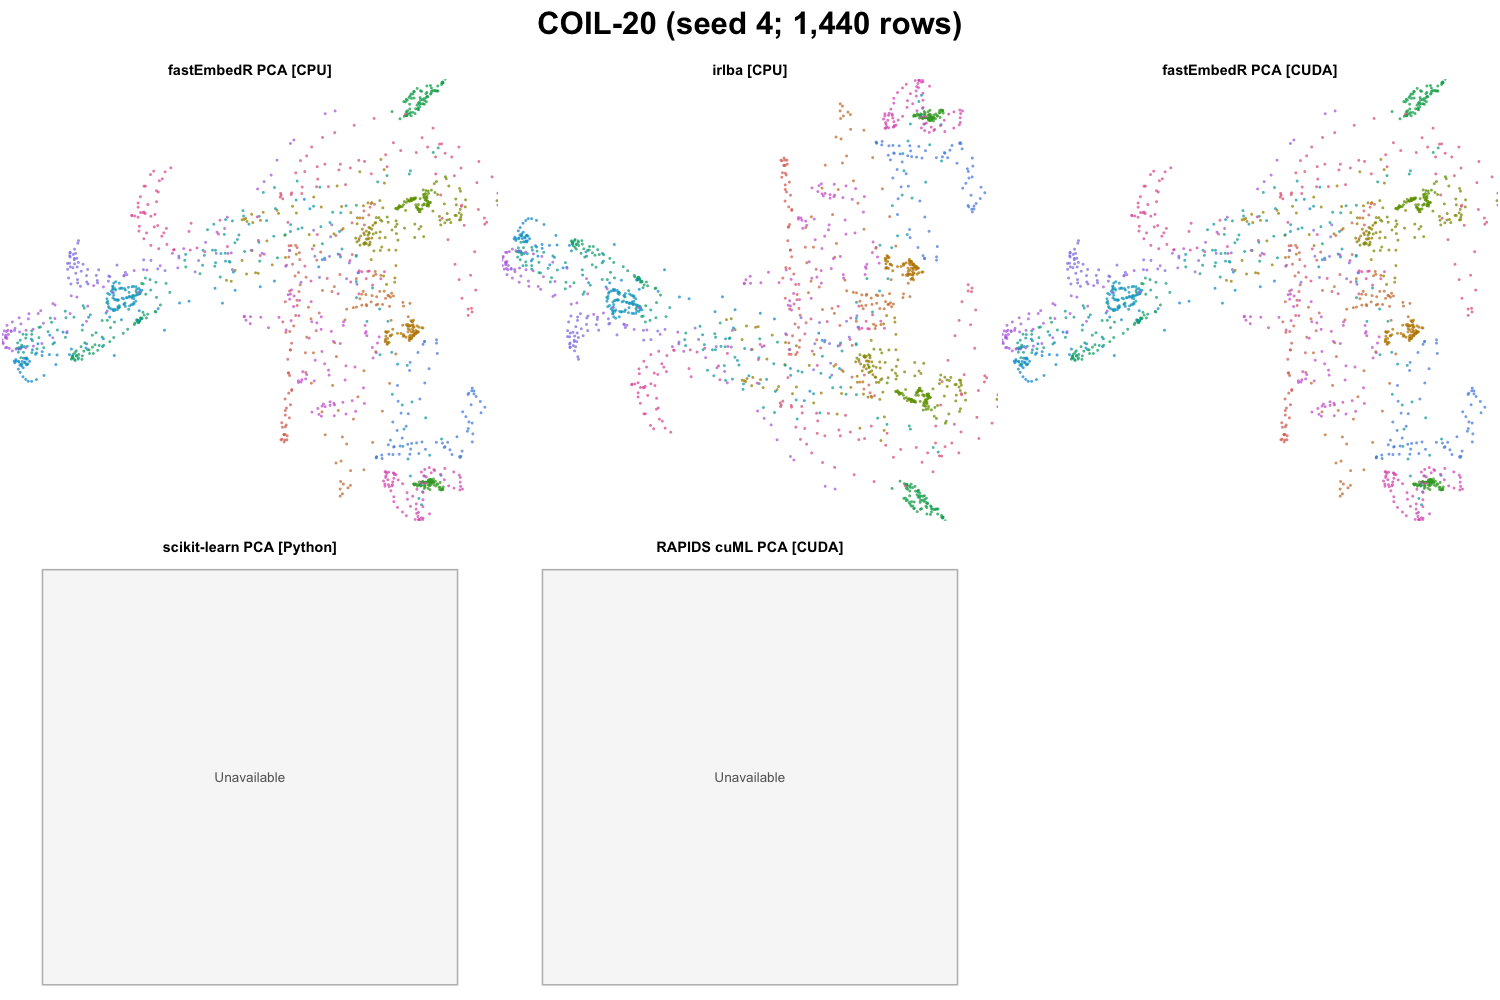
\includegraphics[width=0.94\textwidth]{figures/embedding_all_methods/COIL20_pca.png}
\caption{COIL-20 PCA outputs for the tested methods (seed 4; 1,440 rows). Colors encode benchmark labels and were not used for fitting.}
\end{figure}
\clearpage

\begin{figure}[p]
\centering
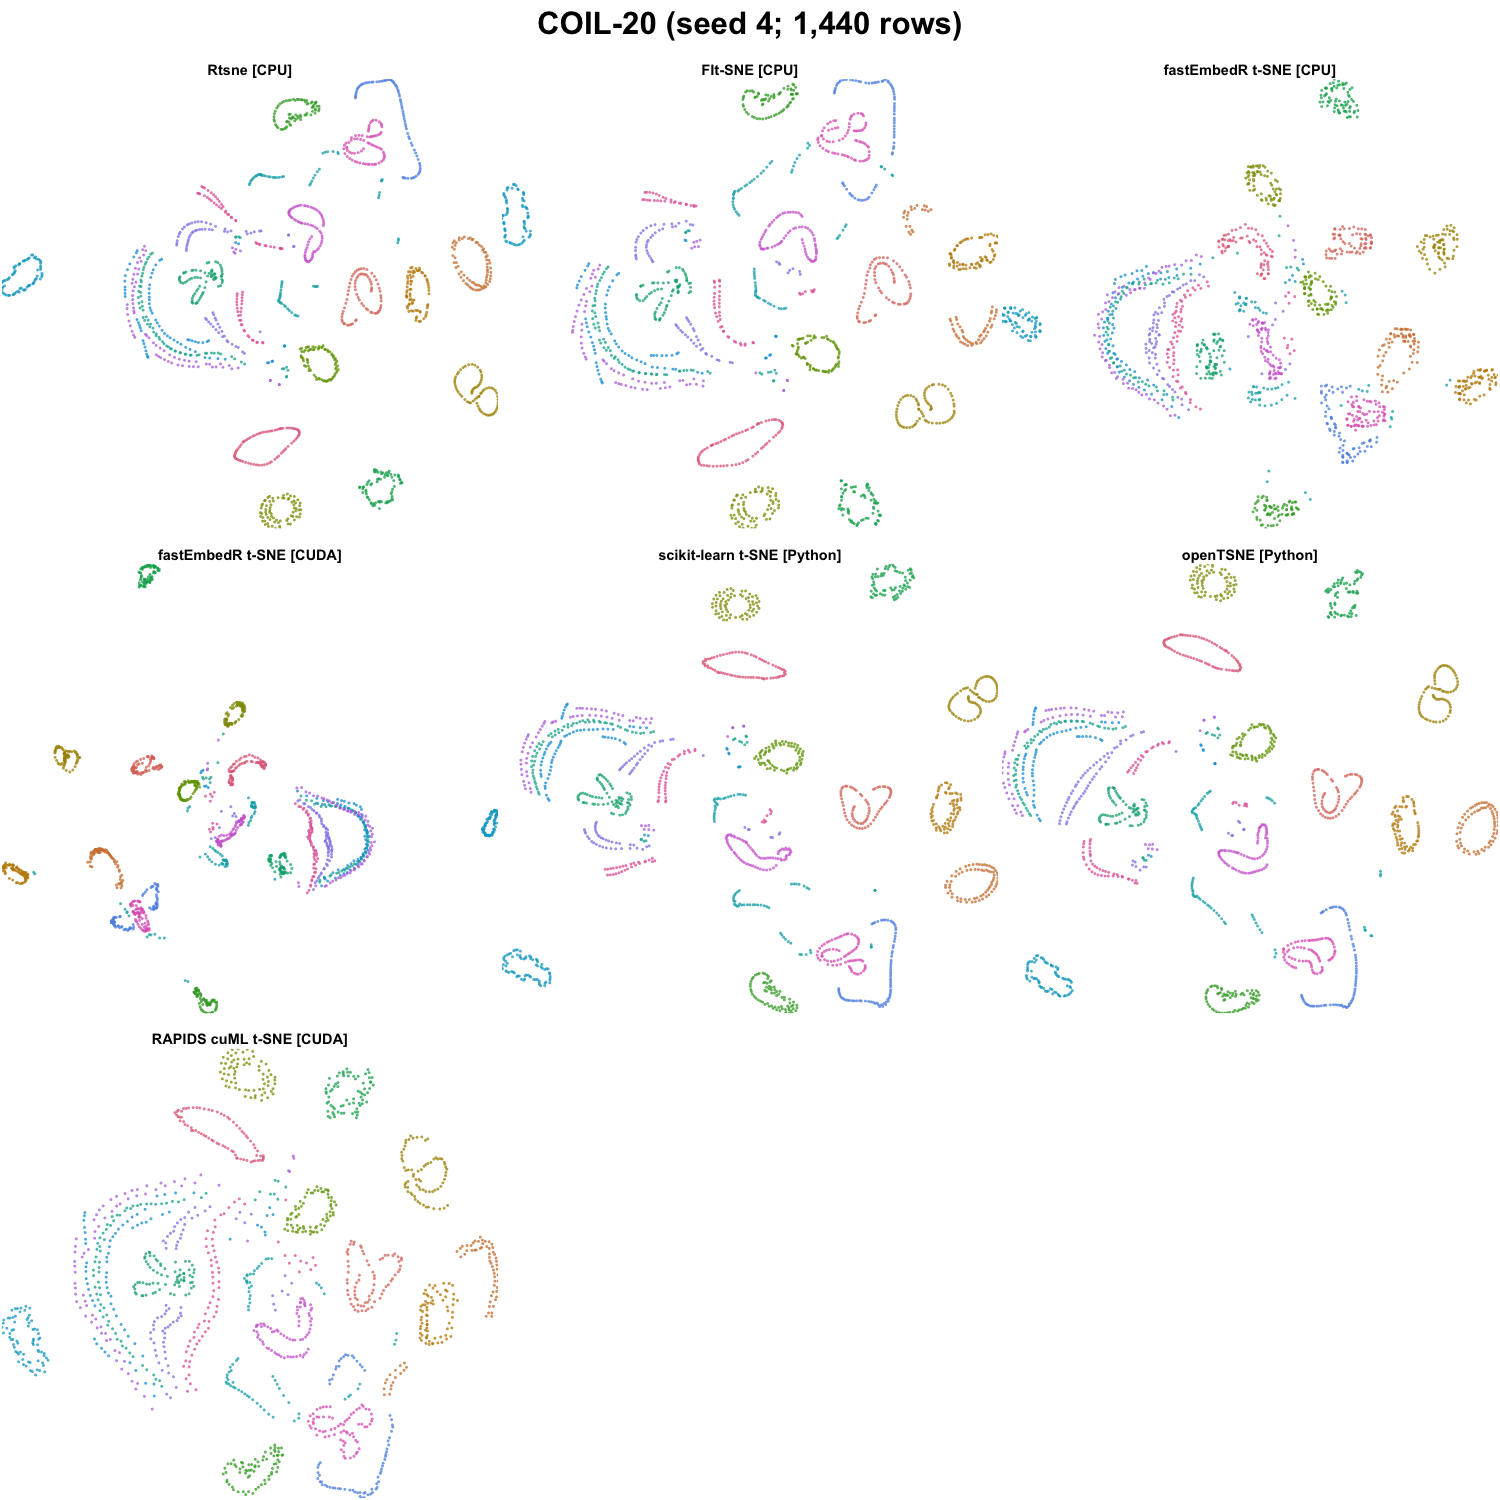
\includegraphics[width=0.94\textwidth]{figures/embedding_all_methods/COIL20_tsne.png}
\caption{COIL-20 t-SNE outputs for the tested methods (seed 4; 1,440 rows). Colors encode benchmark labels and were not used for fitting.}
\end{figure}
\clearpage

\begin{figure}[p]
\centering
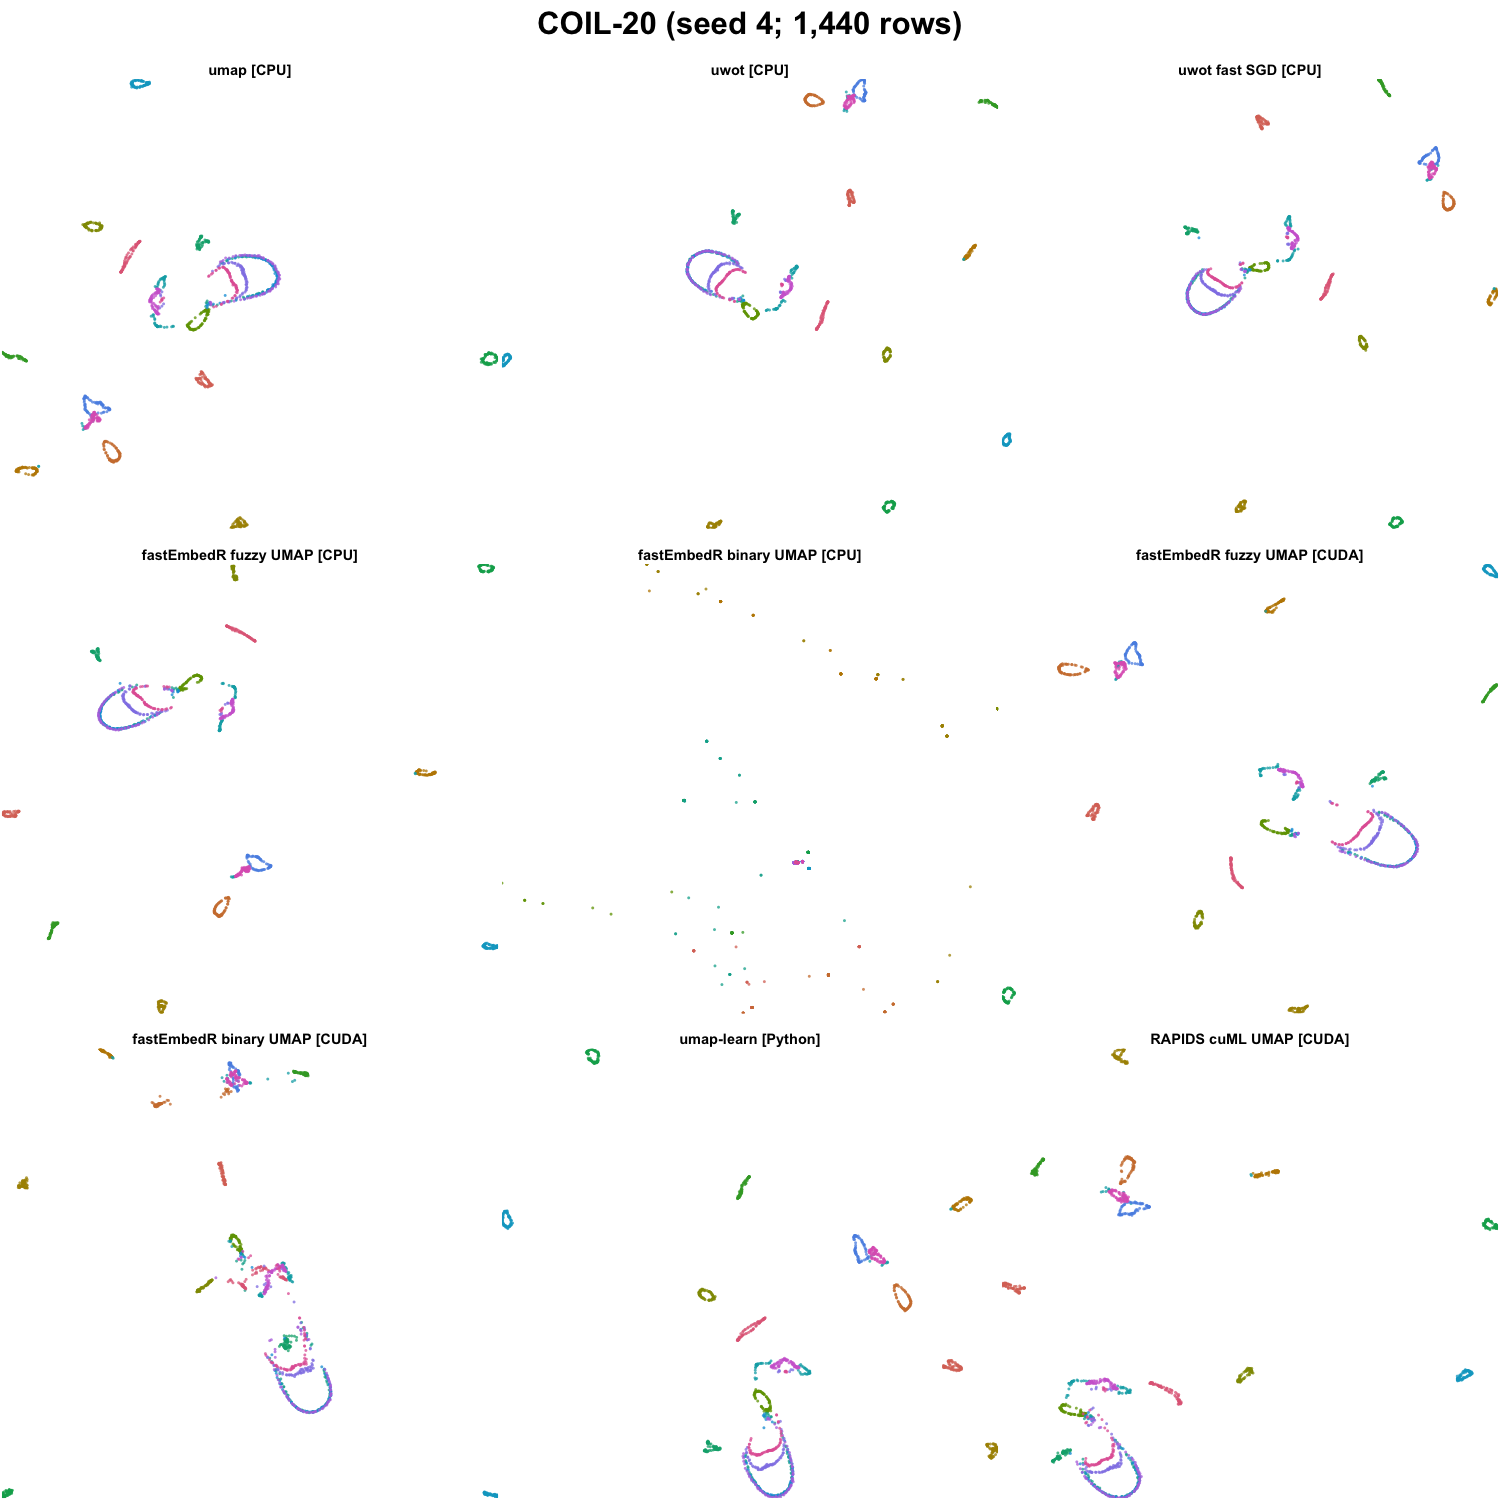
\includegraphics[width=0.94\textwidth]{figures/embedding_all_methods/COIL20_umap.png}
\caption{COIL-20 UMAP outputs for the tested methods (seed 4; 1,440 rows). Colors encode benchmark labels and were not used for fitting.}
\end{figure}
\clearpage

\begin{figure}[p]
\centering
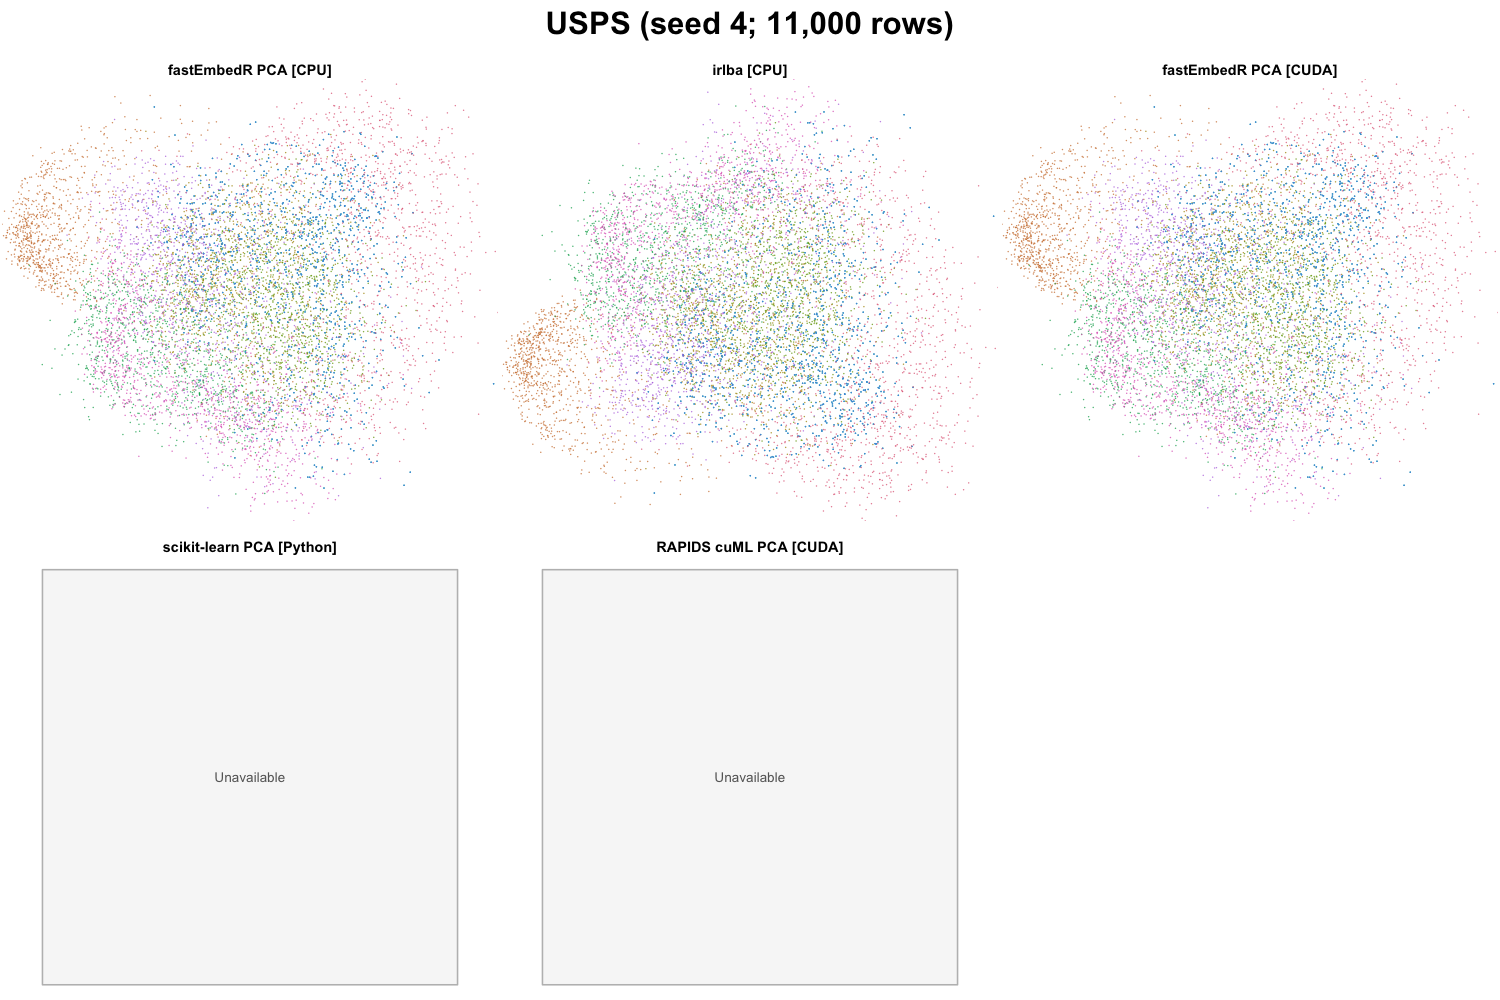
\includegraphics[width=0.94\textwidth]{figures/embedding_all_methods/USPS_pca.png}
\caption{USPS PCA outputs for the tested methods (seed 4; 11,000 rows). Colors encode benchmark labels and were not used for fitting.}
\end{figure}
\clearpage

\begin{figure}[p]
\centering
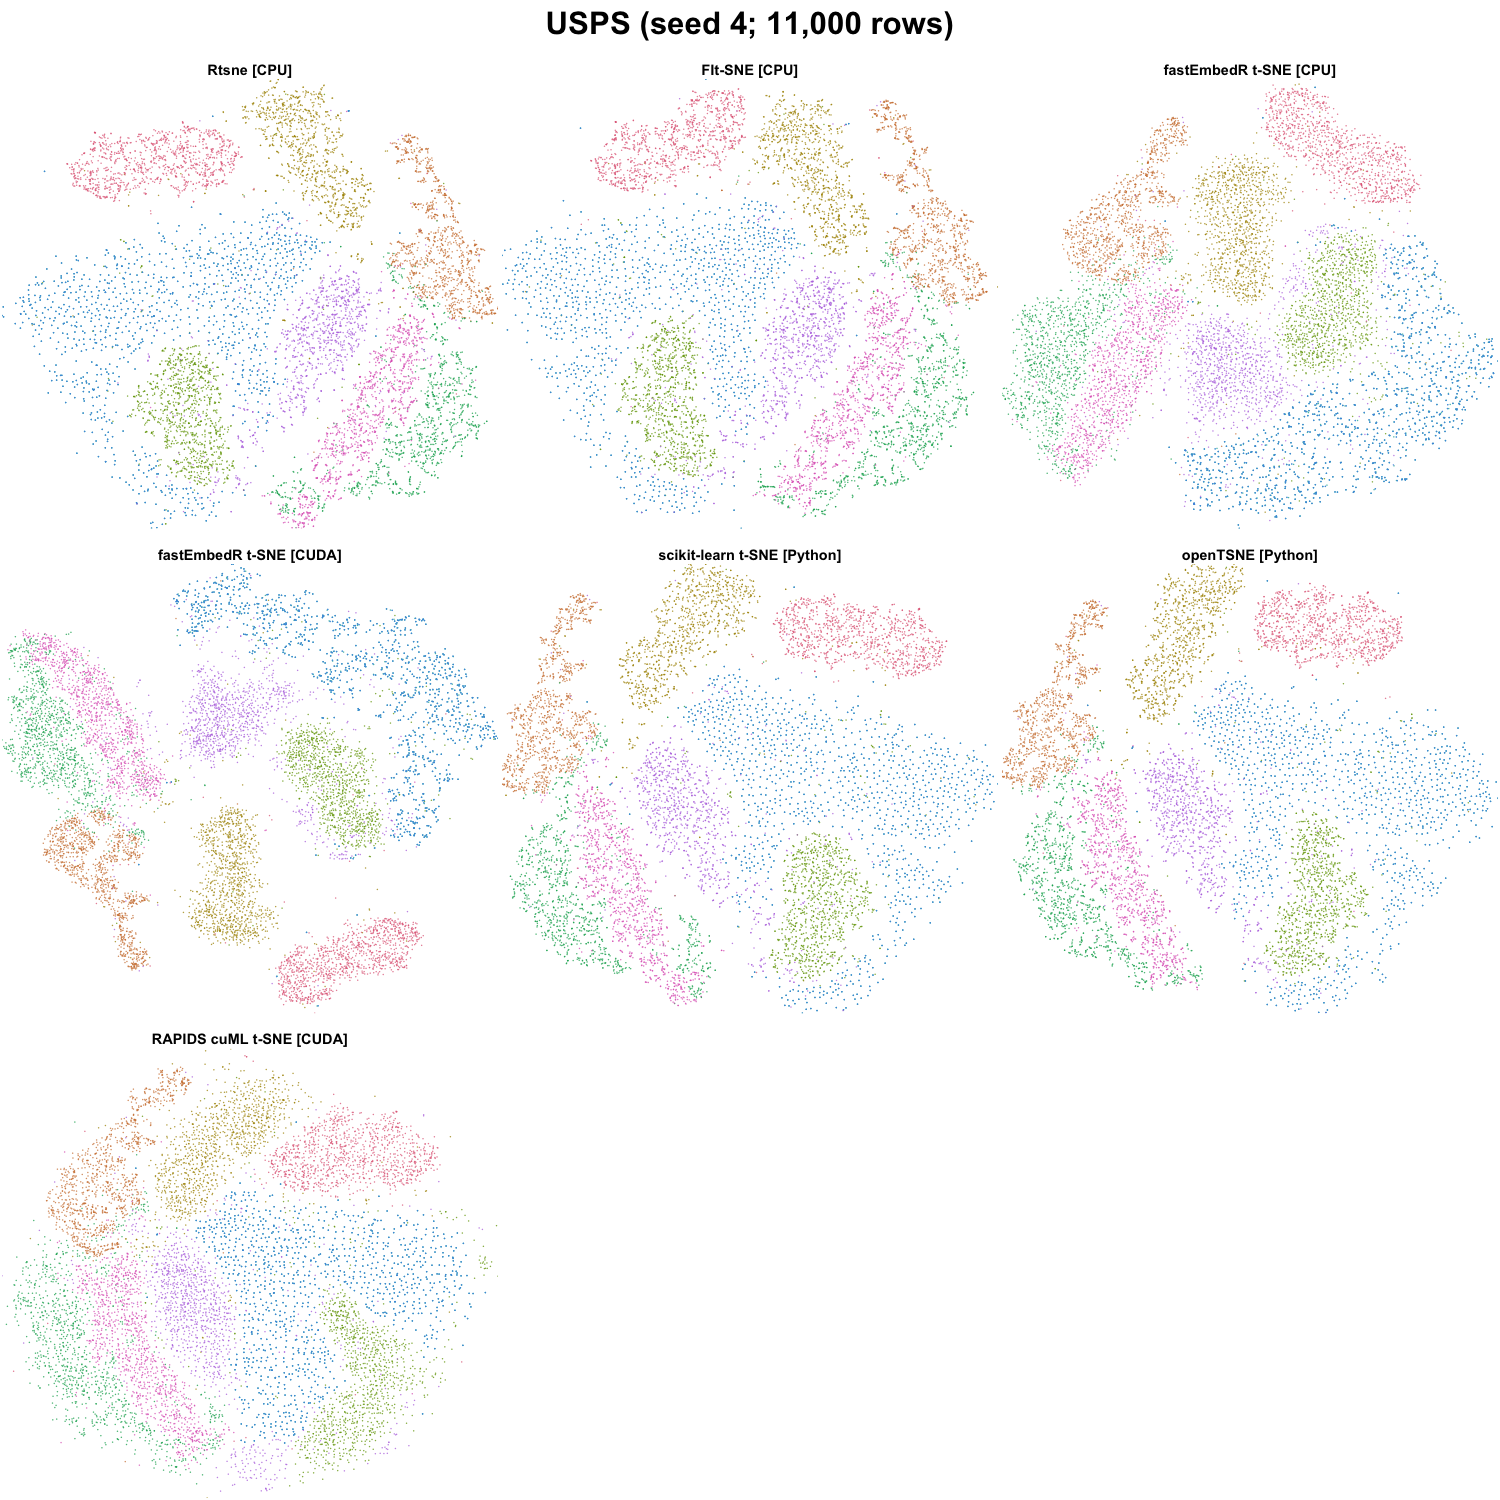
\includegraphics[width=0.94\textwidth]{figures/embedding_all_methods/USPS_tsne.png}
\caption{USPS t-SNE outputs for the tested methods (seed 4; 11,000 rows). Colors encode benchmark labels and were not used for fitting.}
\end{figure}
\clearpage

\begin{figure}[p]
\centering
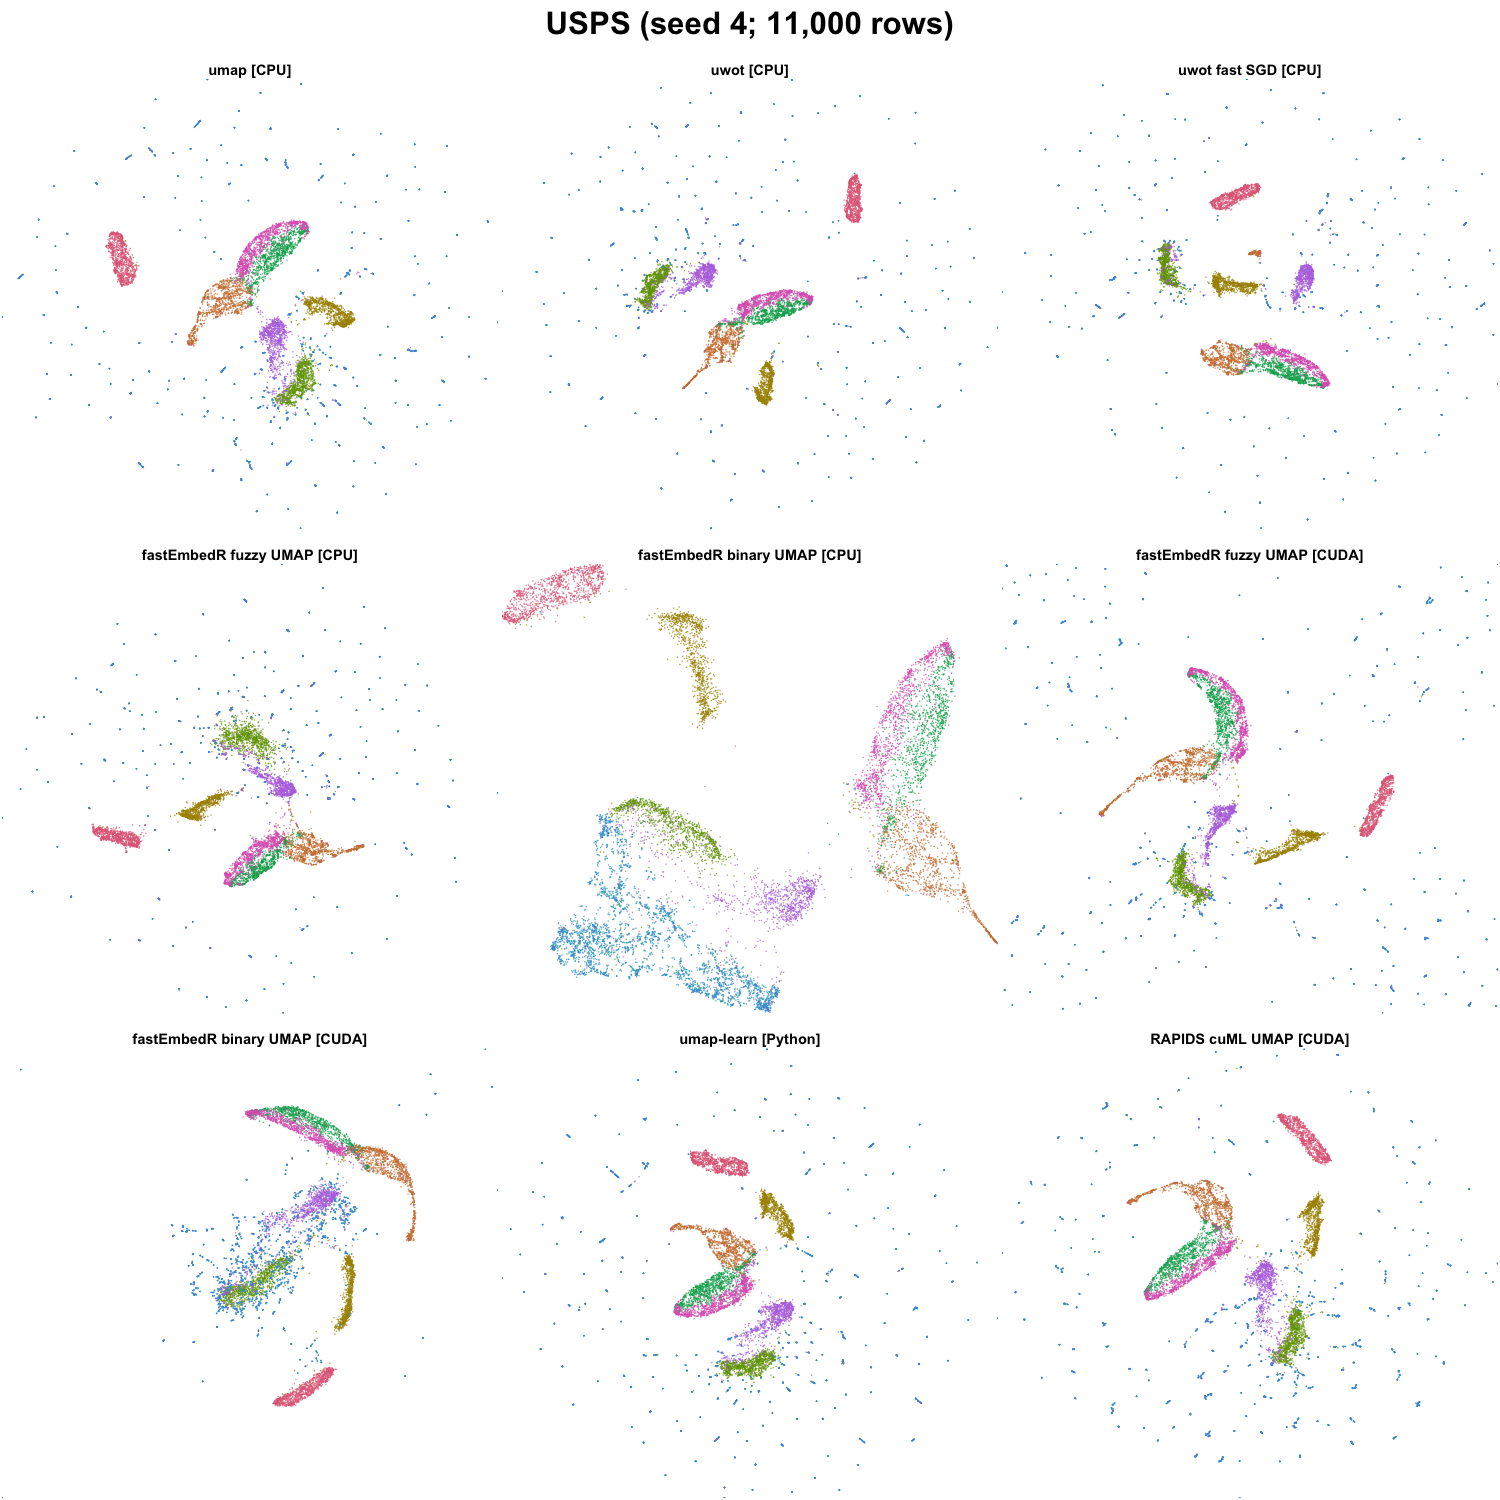
\includegraphics[width=0.94\textwidth]{figures/embedding_all_methods/USPS_umap.png}
\caption{USPS UMAP outputs for the tested methods (seed 4; 11,000 rows). Colors encode benchmark labels and were not used for fitting.}
\end{figure}
\clearpage

\begin{figure}[p]
\centering
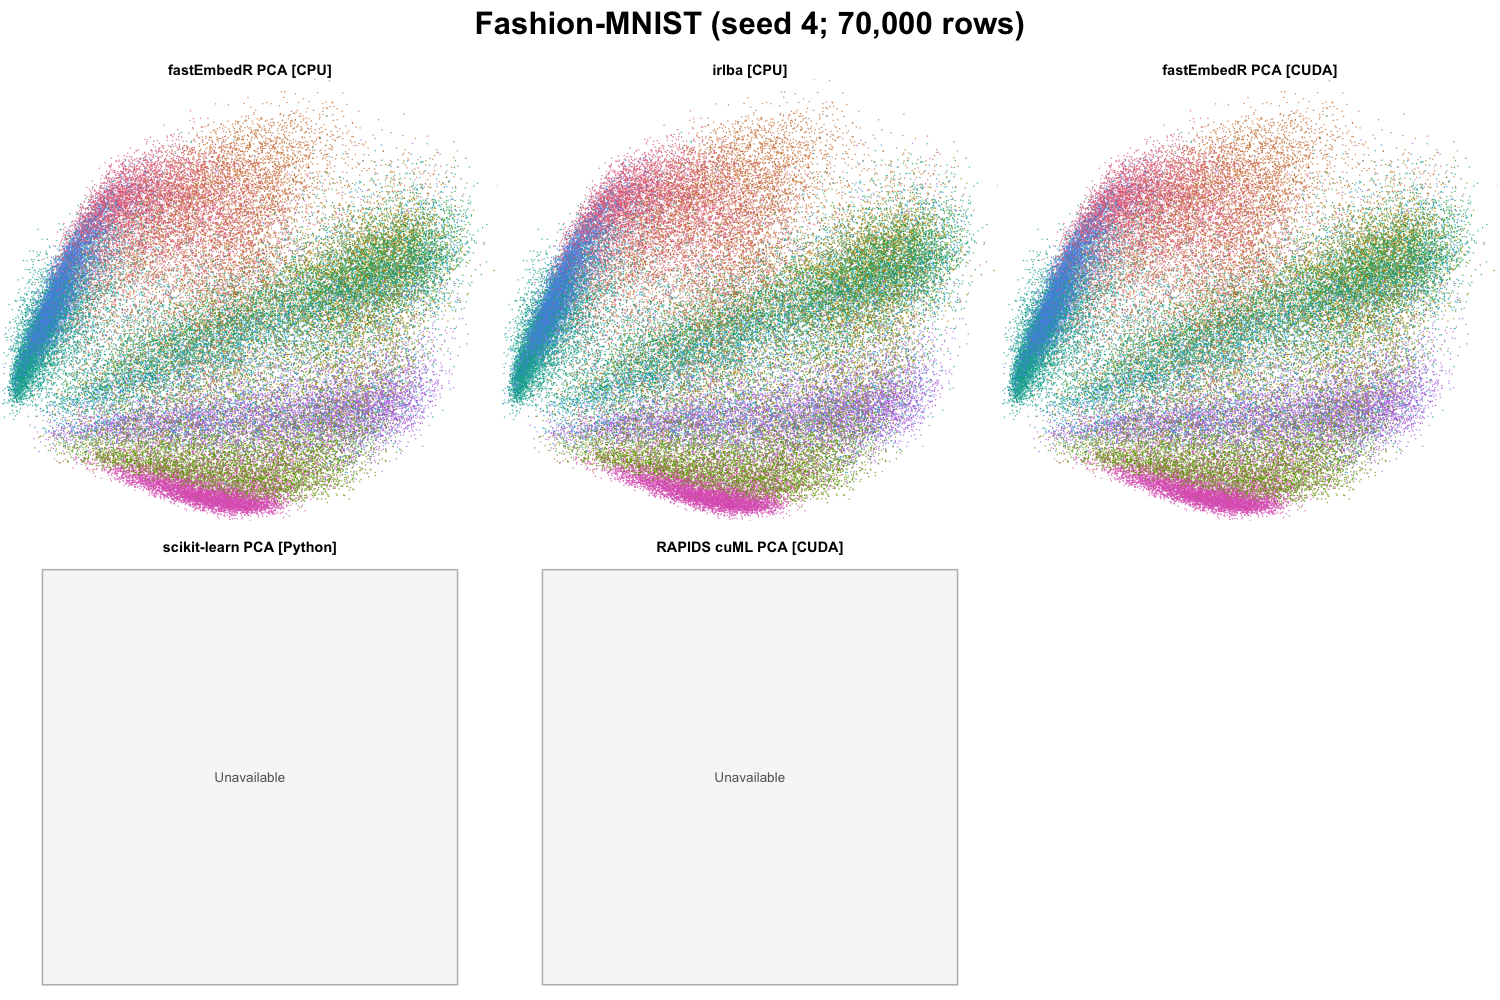
\includegraphics[width=0.94\textwidth]{figures/embedding_all_methods/FashionMNIST_pca.png}
\caption{Fashion-MNIST PCA outputs for the tested methods (seed 4; 70,000 rows). Colors encode benchmark labels and were not used for fitting.}
\end{figure}
\clearpage

\begin{figure}[p]
\centering
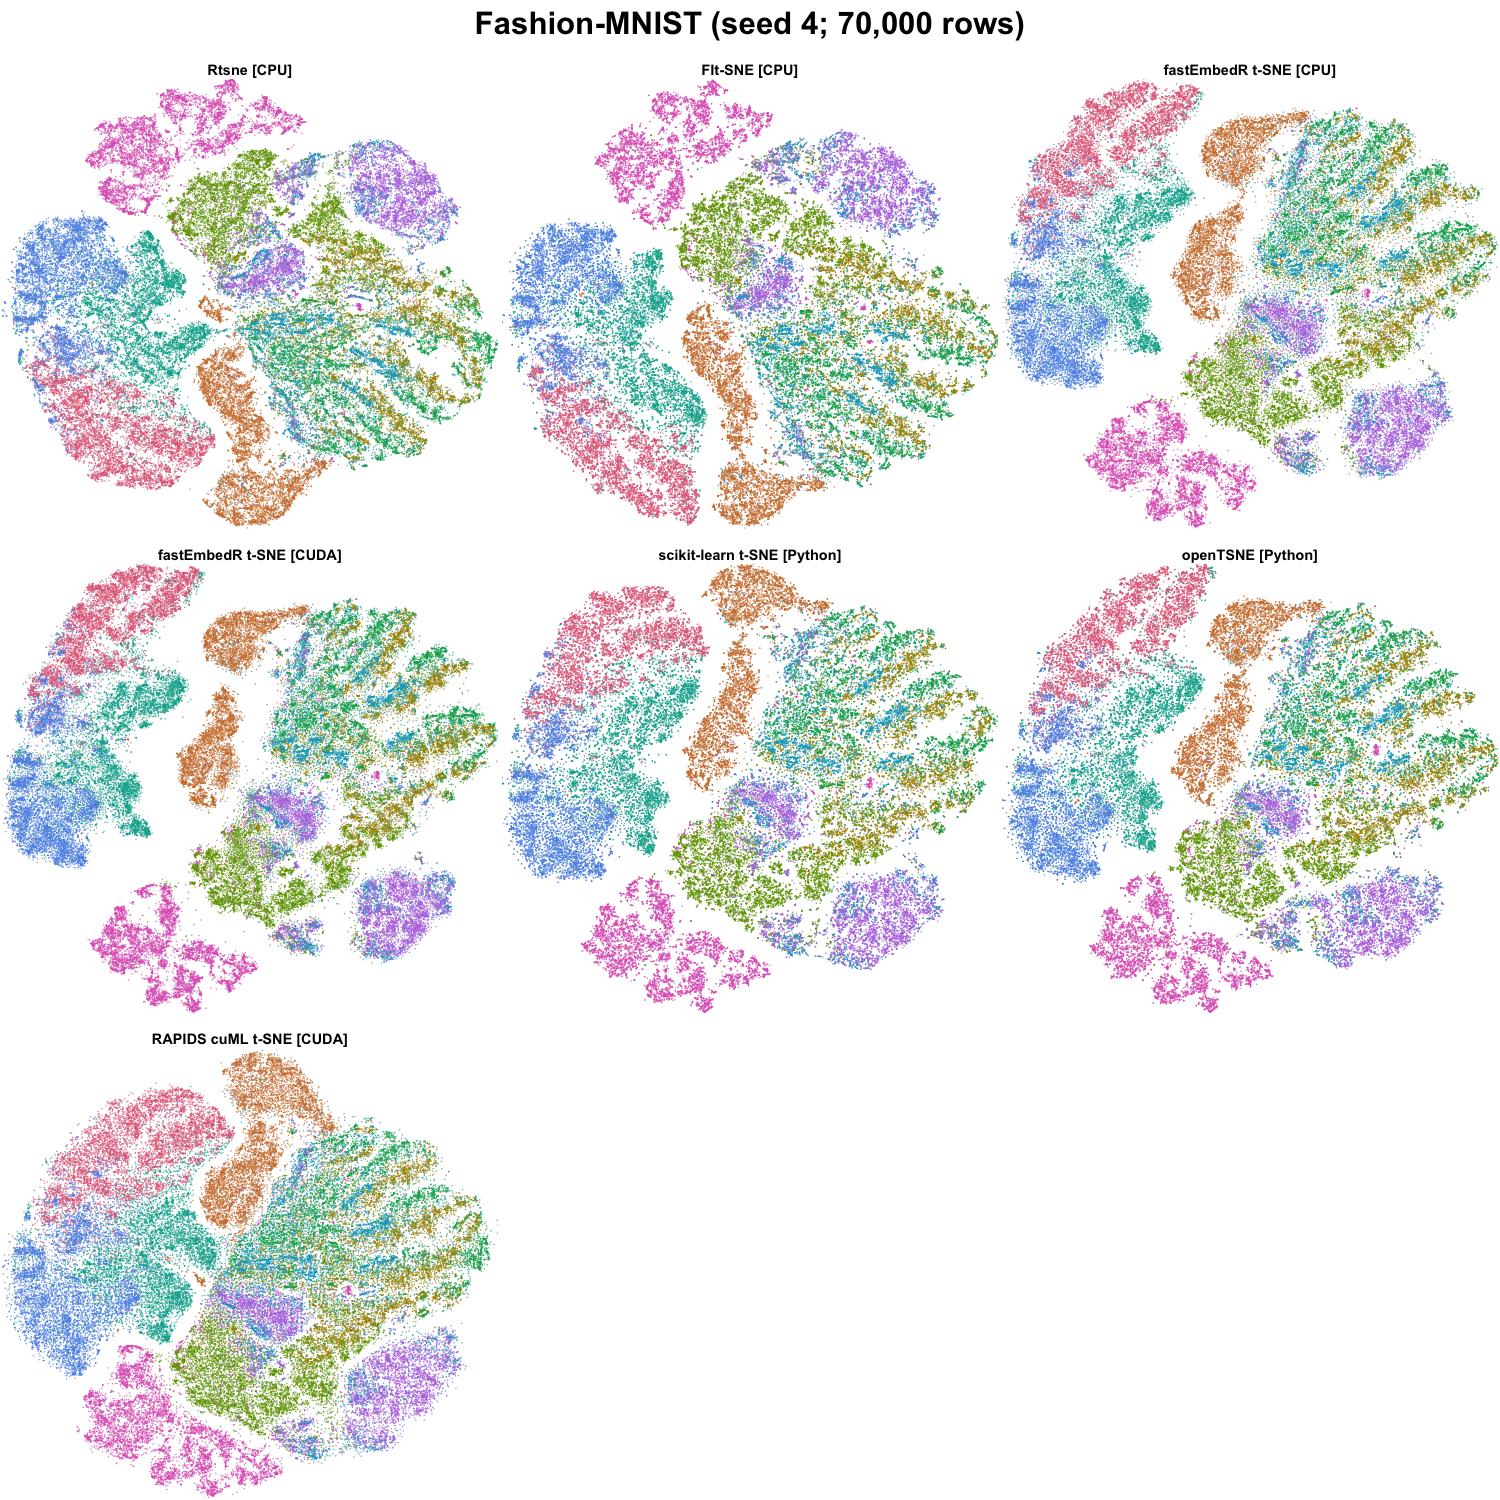
\includegraphics[width=0.94\textwidth]{figures/embedding_all_methods/FashionMNIST_tsne.png}
\caption{Fashion-MNIST t-SNE outputs for the tested methods (seed 4; 70,000 rows). Colors encode benchmark labels and were not used for fitting.}
\end{figure}
\clearpage

\begin{figure}[p]
\centering
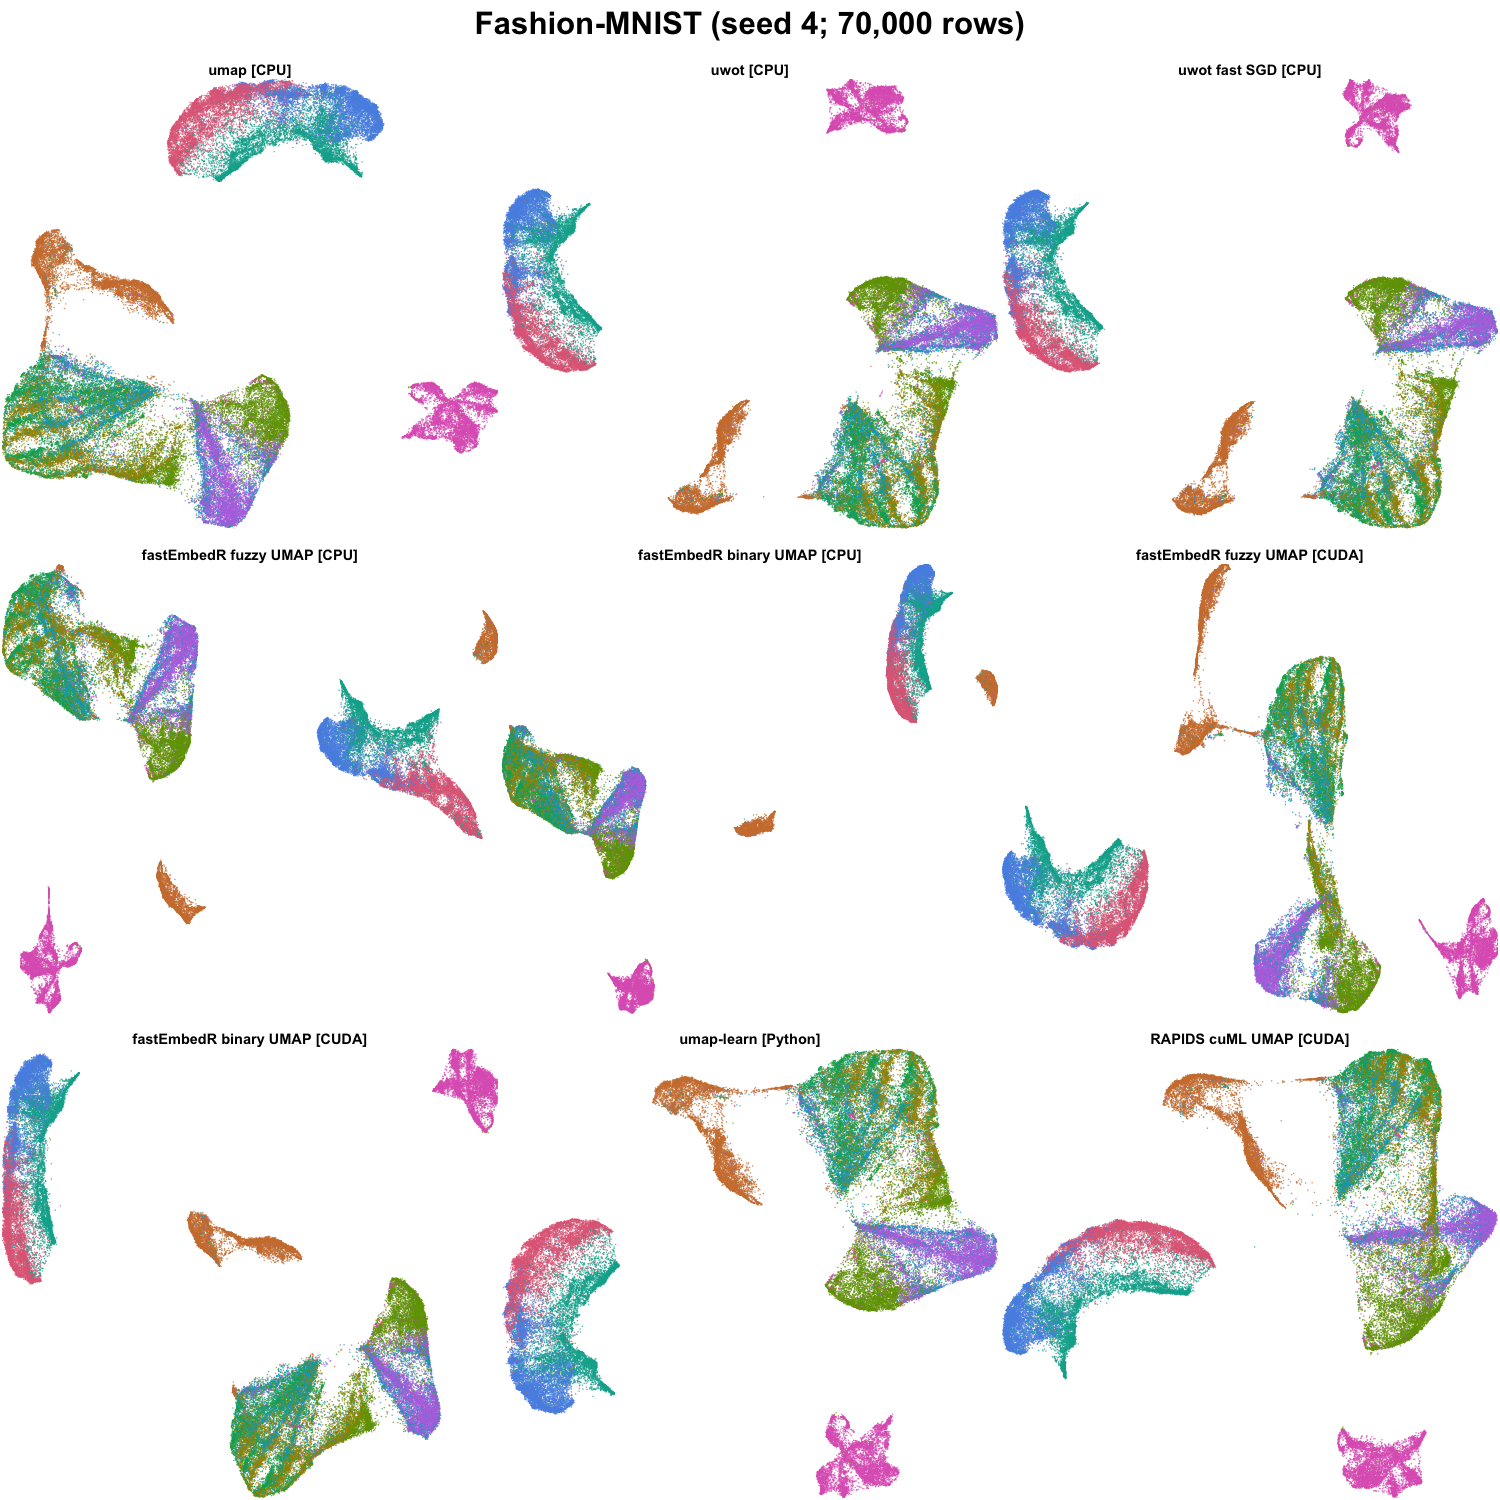
\includegraphics[width=0.94\textwidth]{figures/embedding_all_methods/FashionMNIST_umap.png}
\caption{Fashion-MNIST UMAP outputs for the tested methods (seed 4; 70,000 rows). Colors encode benchmark labels and were not used for fitting.}
\end{figure}
\clearpage

\begin{figure}[p]
\centering
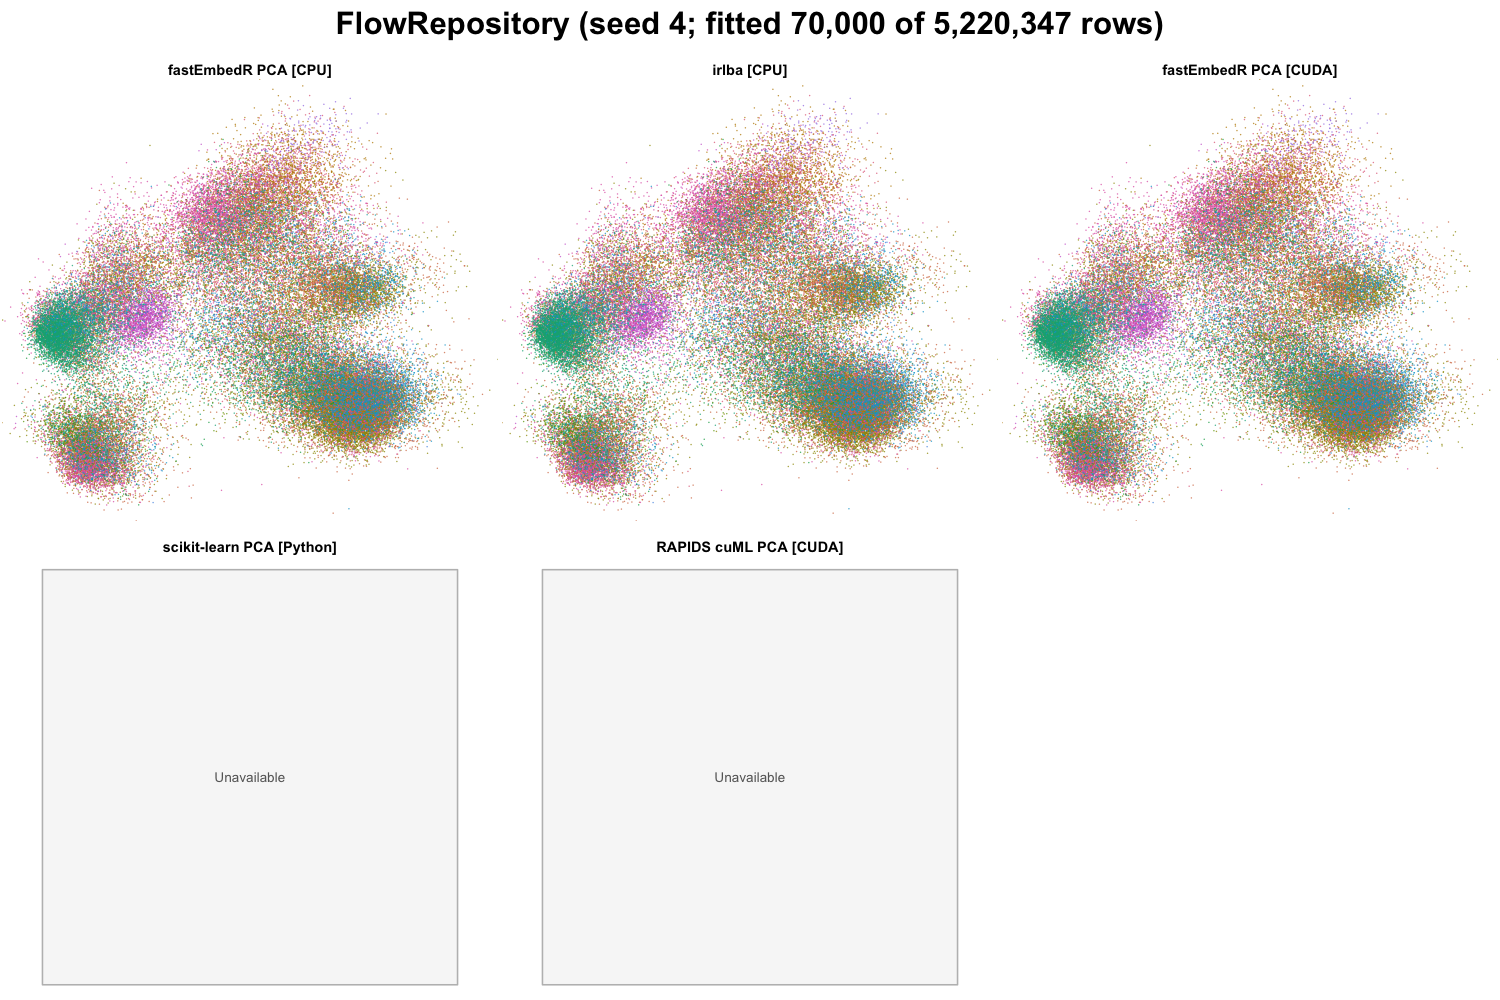
\includegraphics[width=0.94\textwidth]{figures/embedding_all_methods/FlowRepository_FR_FCM_ZYRM_files_pca.png}
\caption{FlowRepository PCA outputs for the tested methods (seed 4; fitted 70,000 of 5,220,347 rows). Colors encode benchmark labels and were not used for fitting.}
\end{figure}
\clearpage

\begin{figure}[p]
\centering
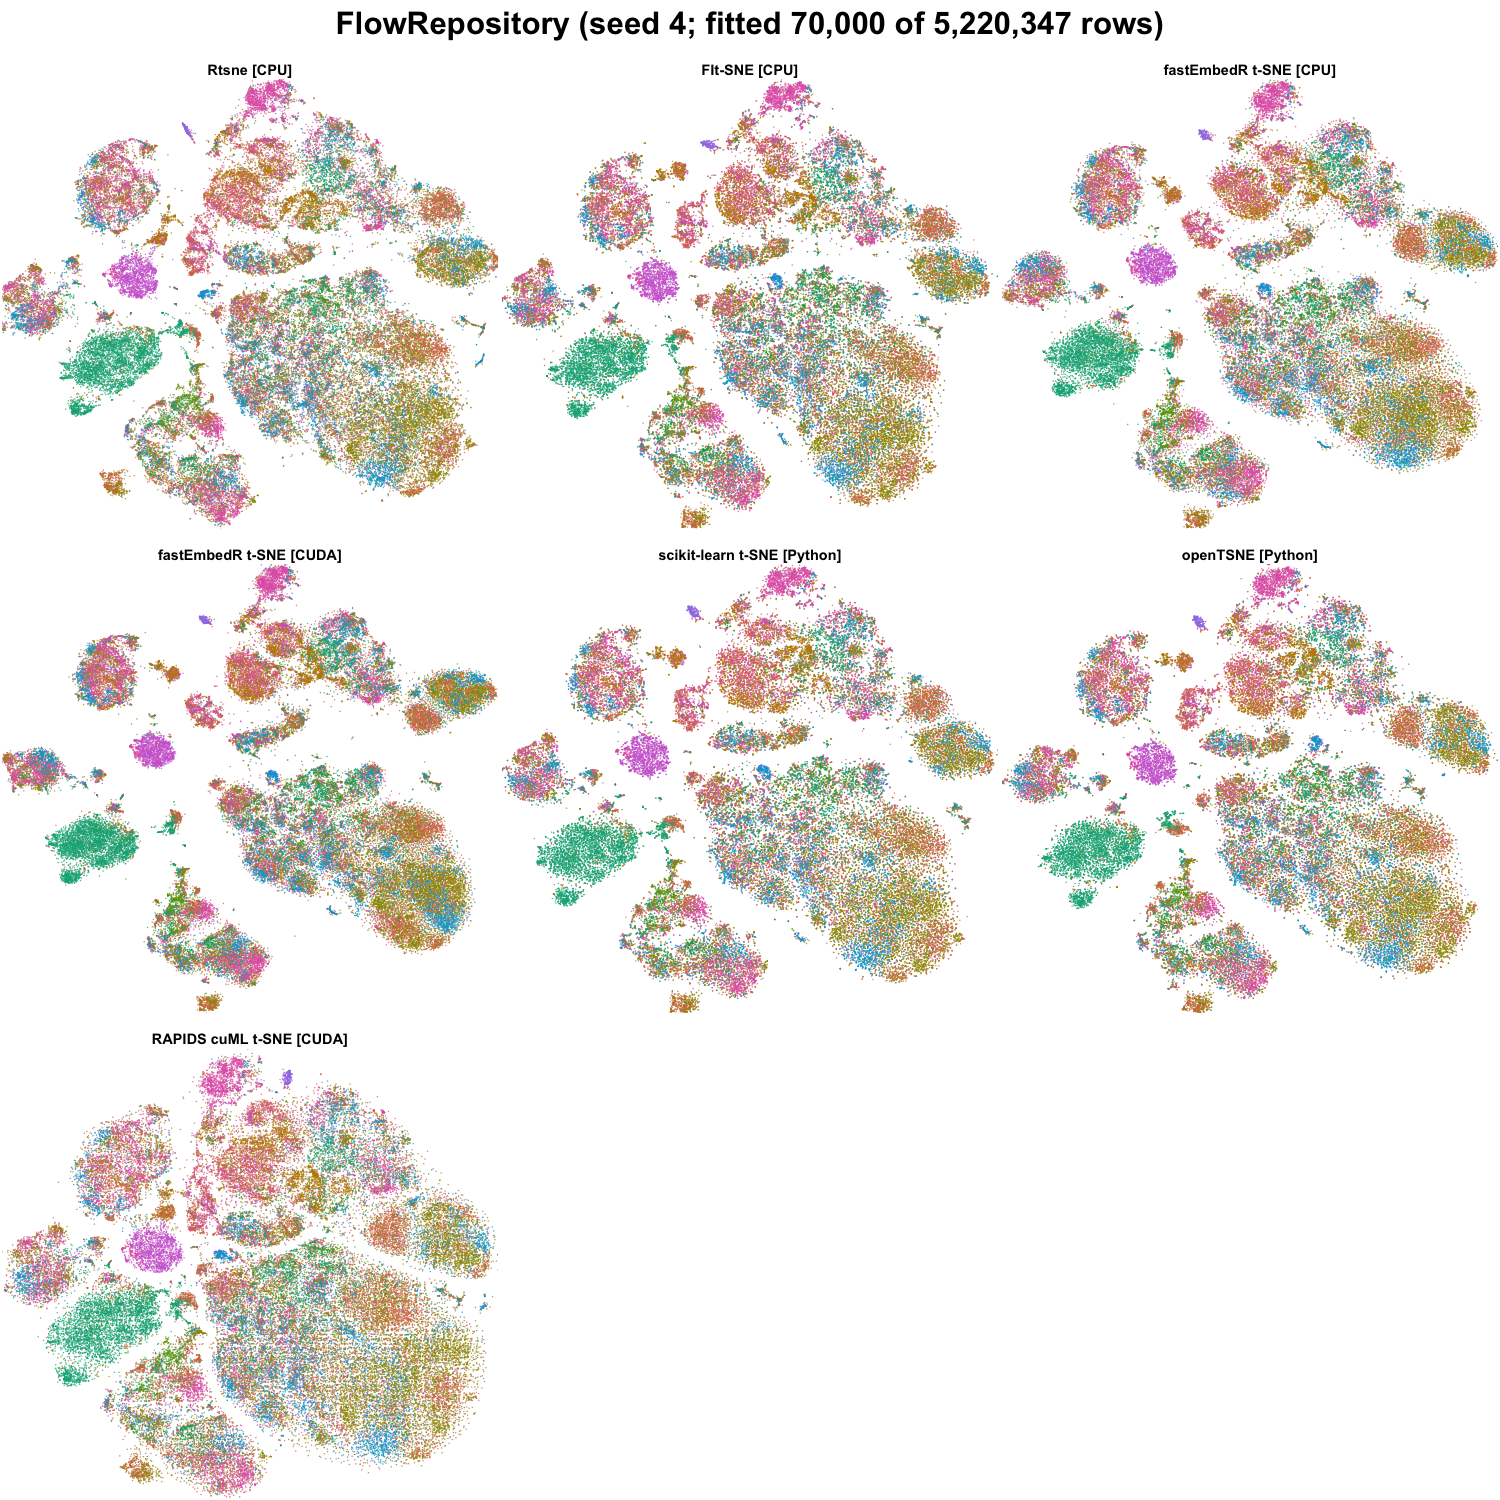
\includegraphics[width=0.94\textwidth]{figures/embedding_all_methods/FlowRepository_FR_FCM_ZYRM_files_tsne.png}
\caption{FlowRepository t-SNE outputs for the tested methods (seed 4; fitted 70,000 of 5,220,347 rows). Colors encode benchmark labels and were not used for fitting.}
\end{figure}
\clearpage

\begin{figure}[p]
\centering
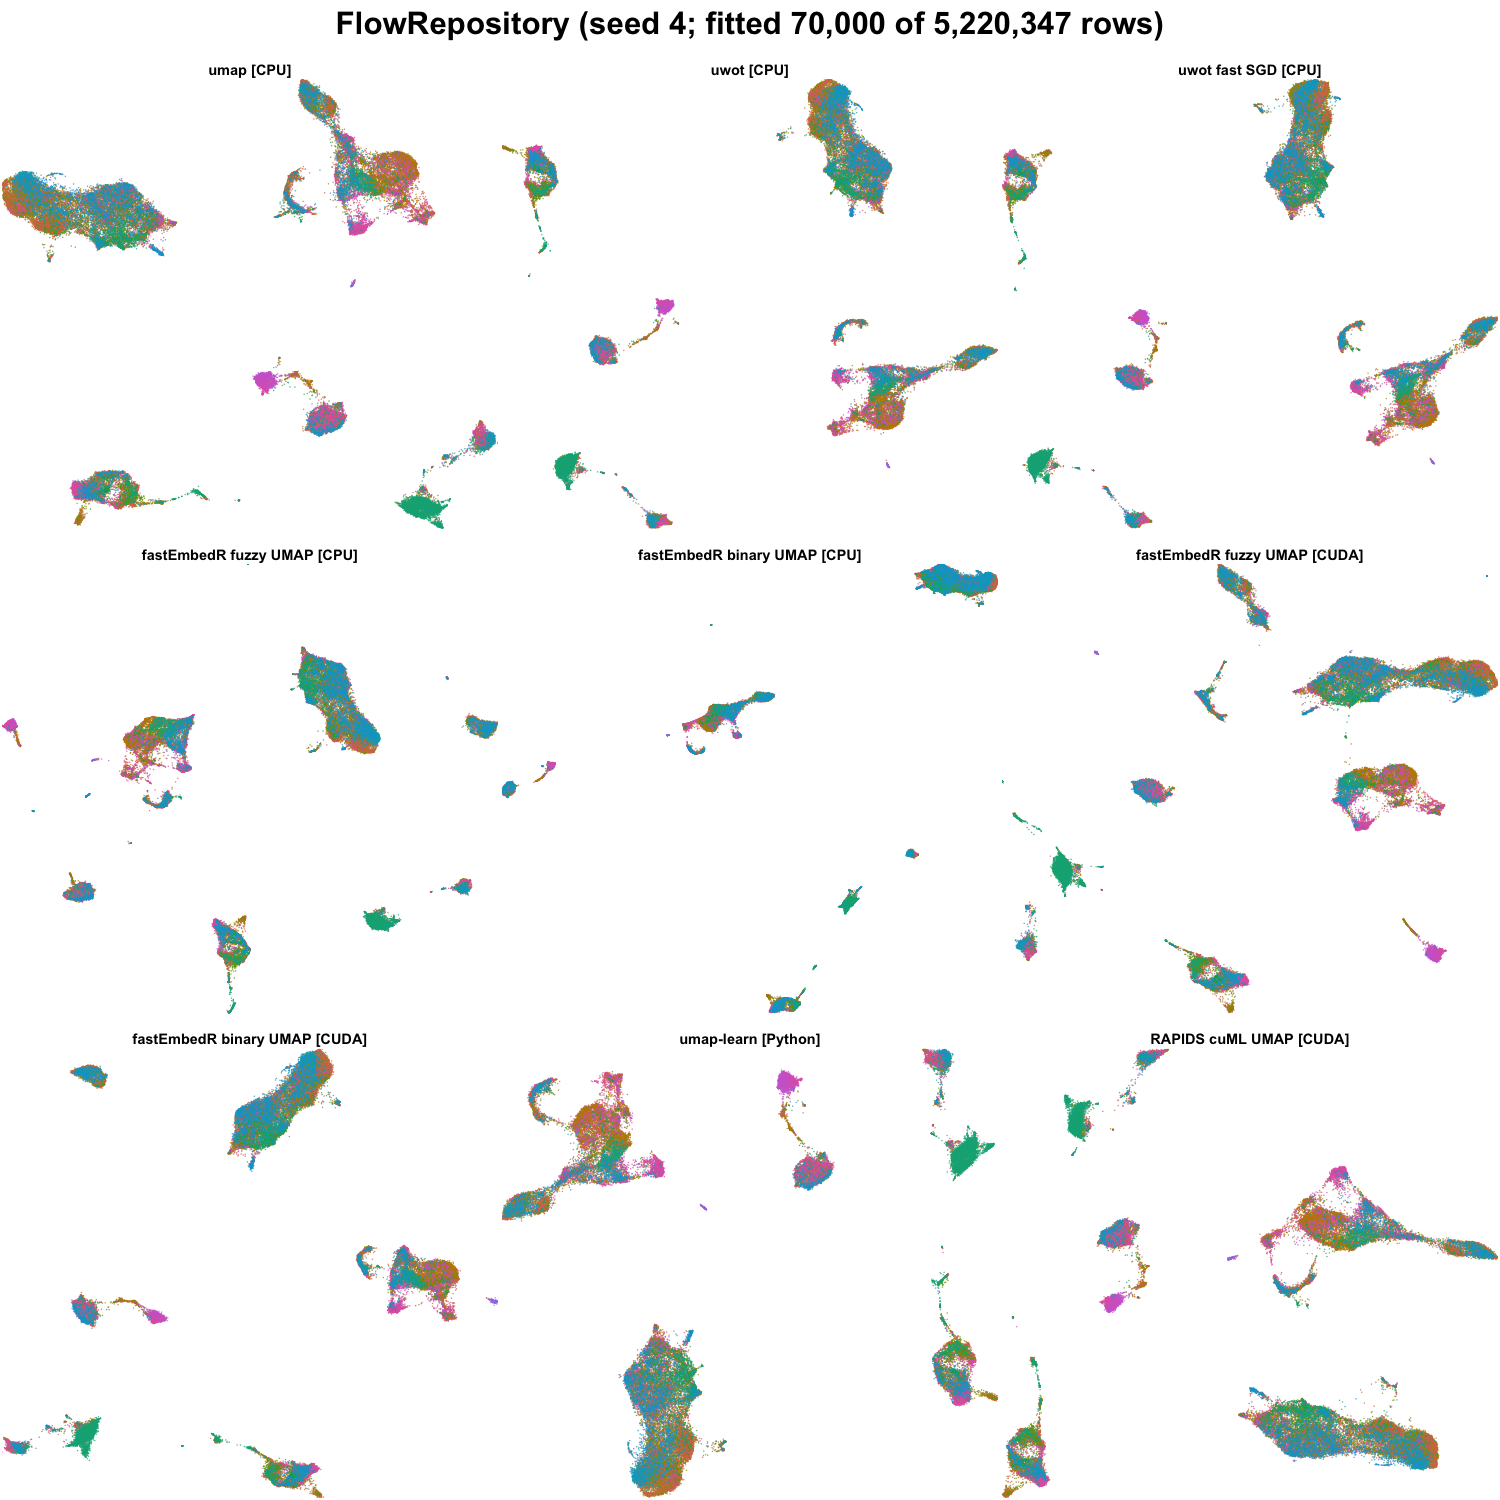
\includegraphics[width=0.94\textwidth]{figures/embedding_all_methods/FlowRepository_FR_FCM_ZYRM_files_umap.png}
\caption{FlowRepository UMAP outputs for the tested methods (seed 4; fitted 70,000 of 5,220,347 rows). Colors encode benchmark labels and were not used for fitting.}
\end{figure}
\clearpage

\begin{figure}[p]
\centering
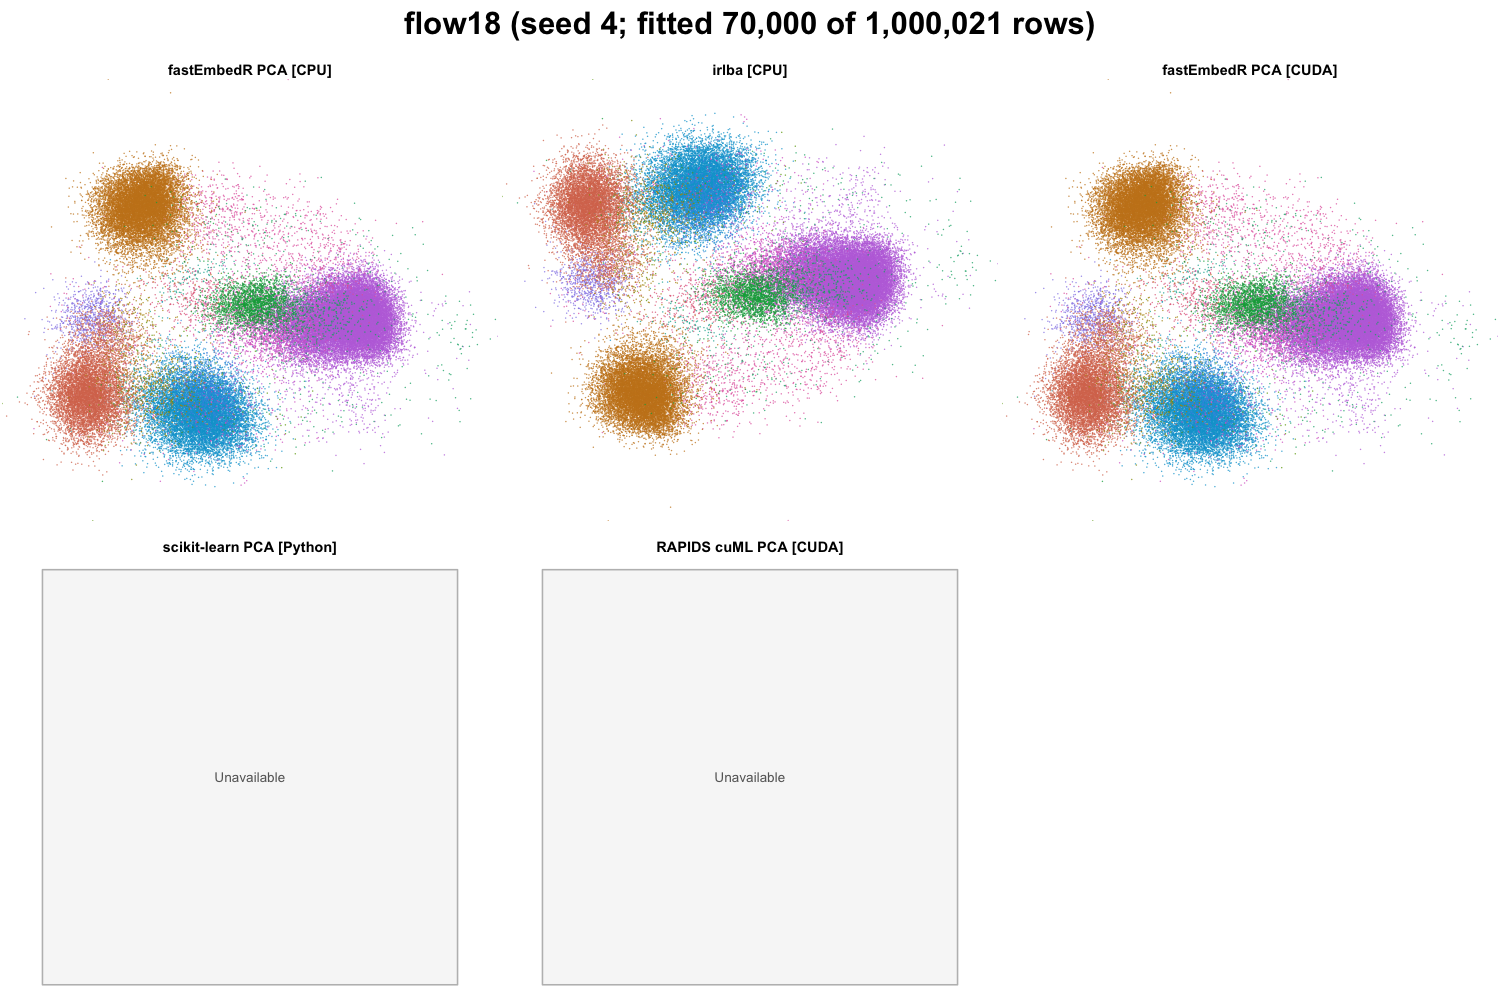
\includegraphics[width=0.94\textwidth]{figures/embedding_all_methods/flow18_pca.png}
\caption{flow18 PCA outputs for the tested methods (seed 4; fitted 70,000 of 1,000,021 rows). Colors encode benchmark labels and were not used for fitting.}
\end{figure}
\clearpage

\begin{figure}[p]
\centering
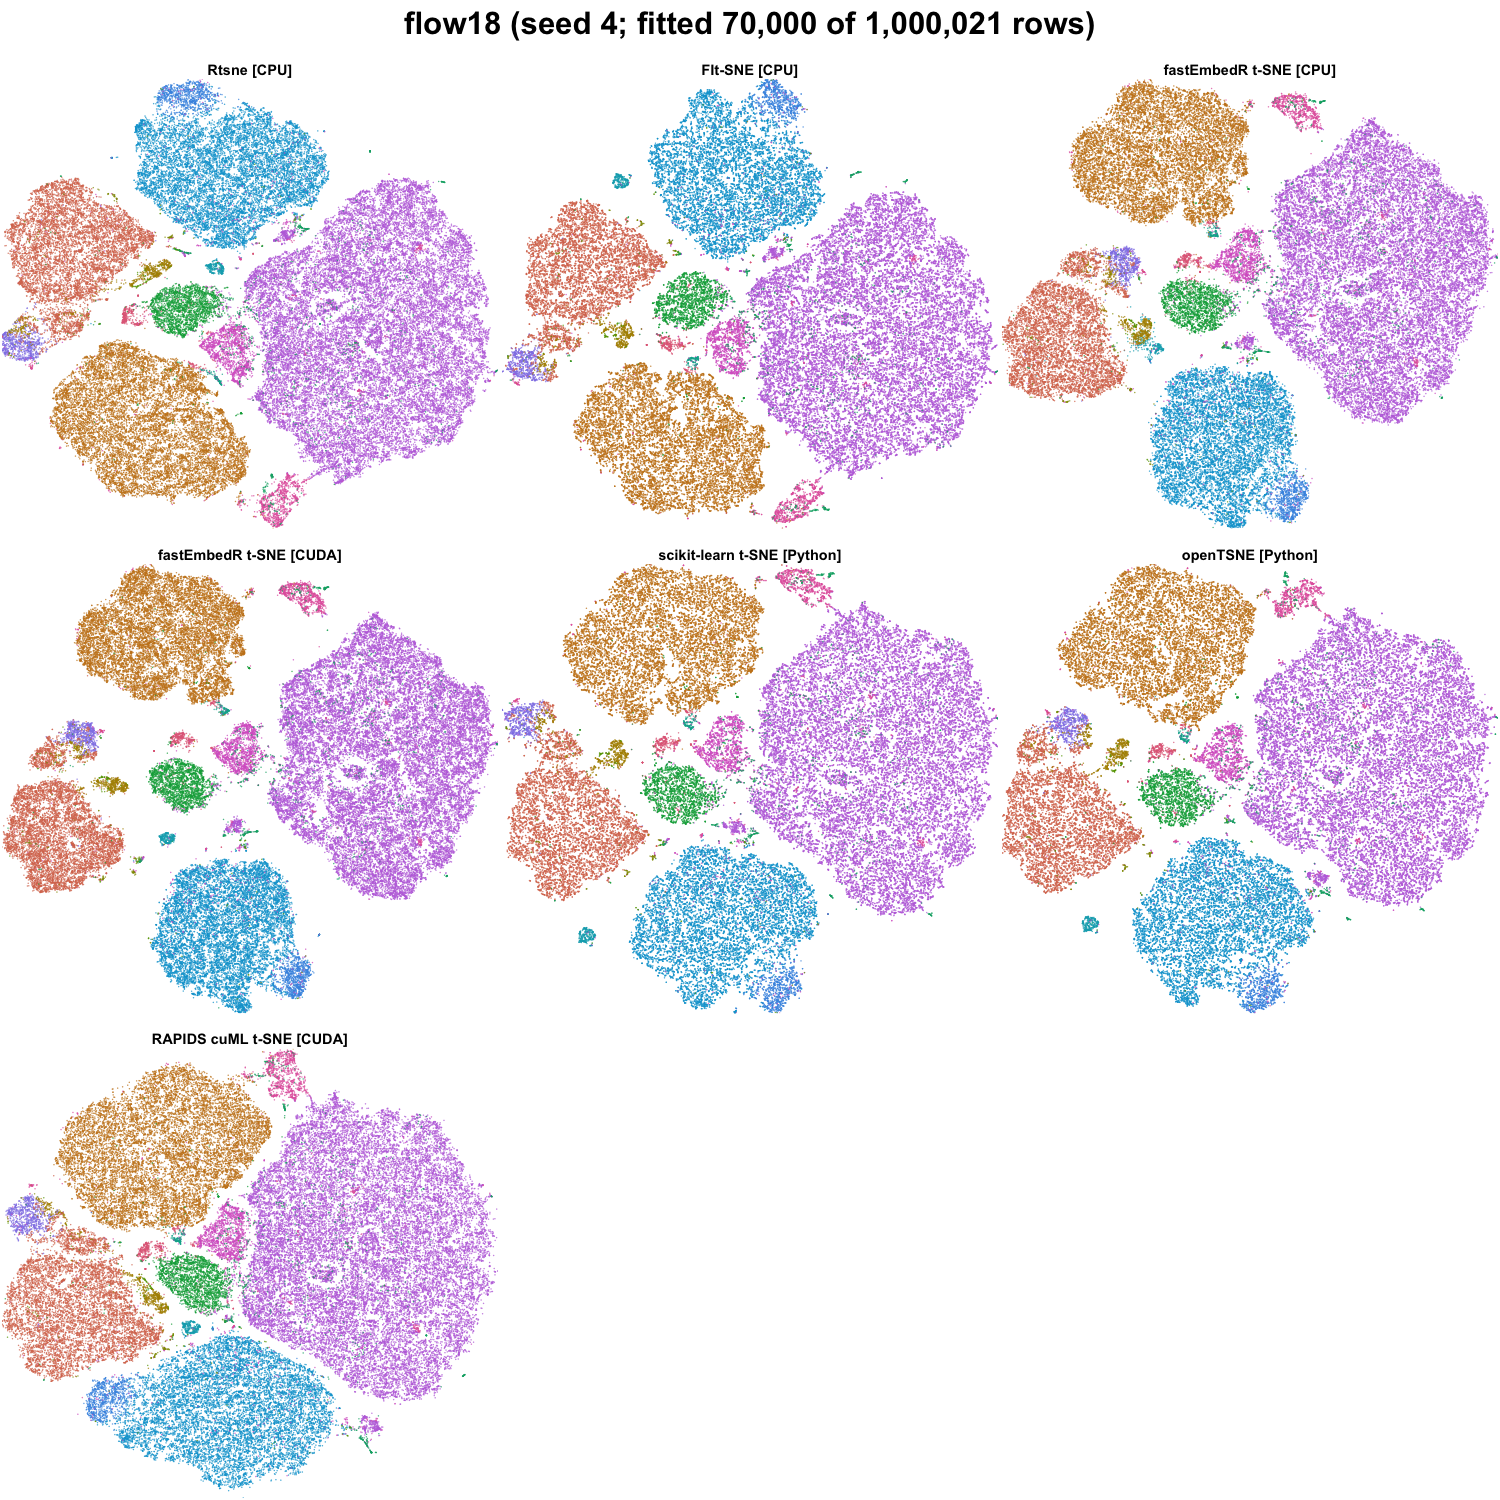
\includegraphics[width=0.94\textwidth]{figures/embedding_all_methods/flow18_tsne.png}
\caption{flow18 t-SNE outputs for the tested methods (seed 4; fitted 70,000 of 1,000,021 rows). Colors encode benchmark labels and were not used for fitting.}
\end{figure}
\clearpage

\begin{figure}[p]
\centering
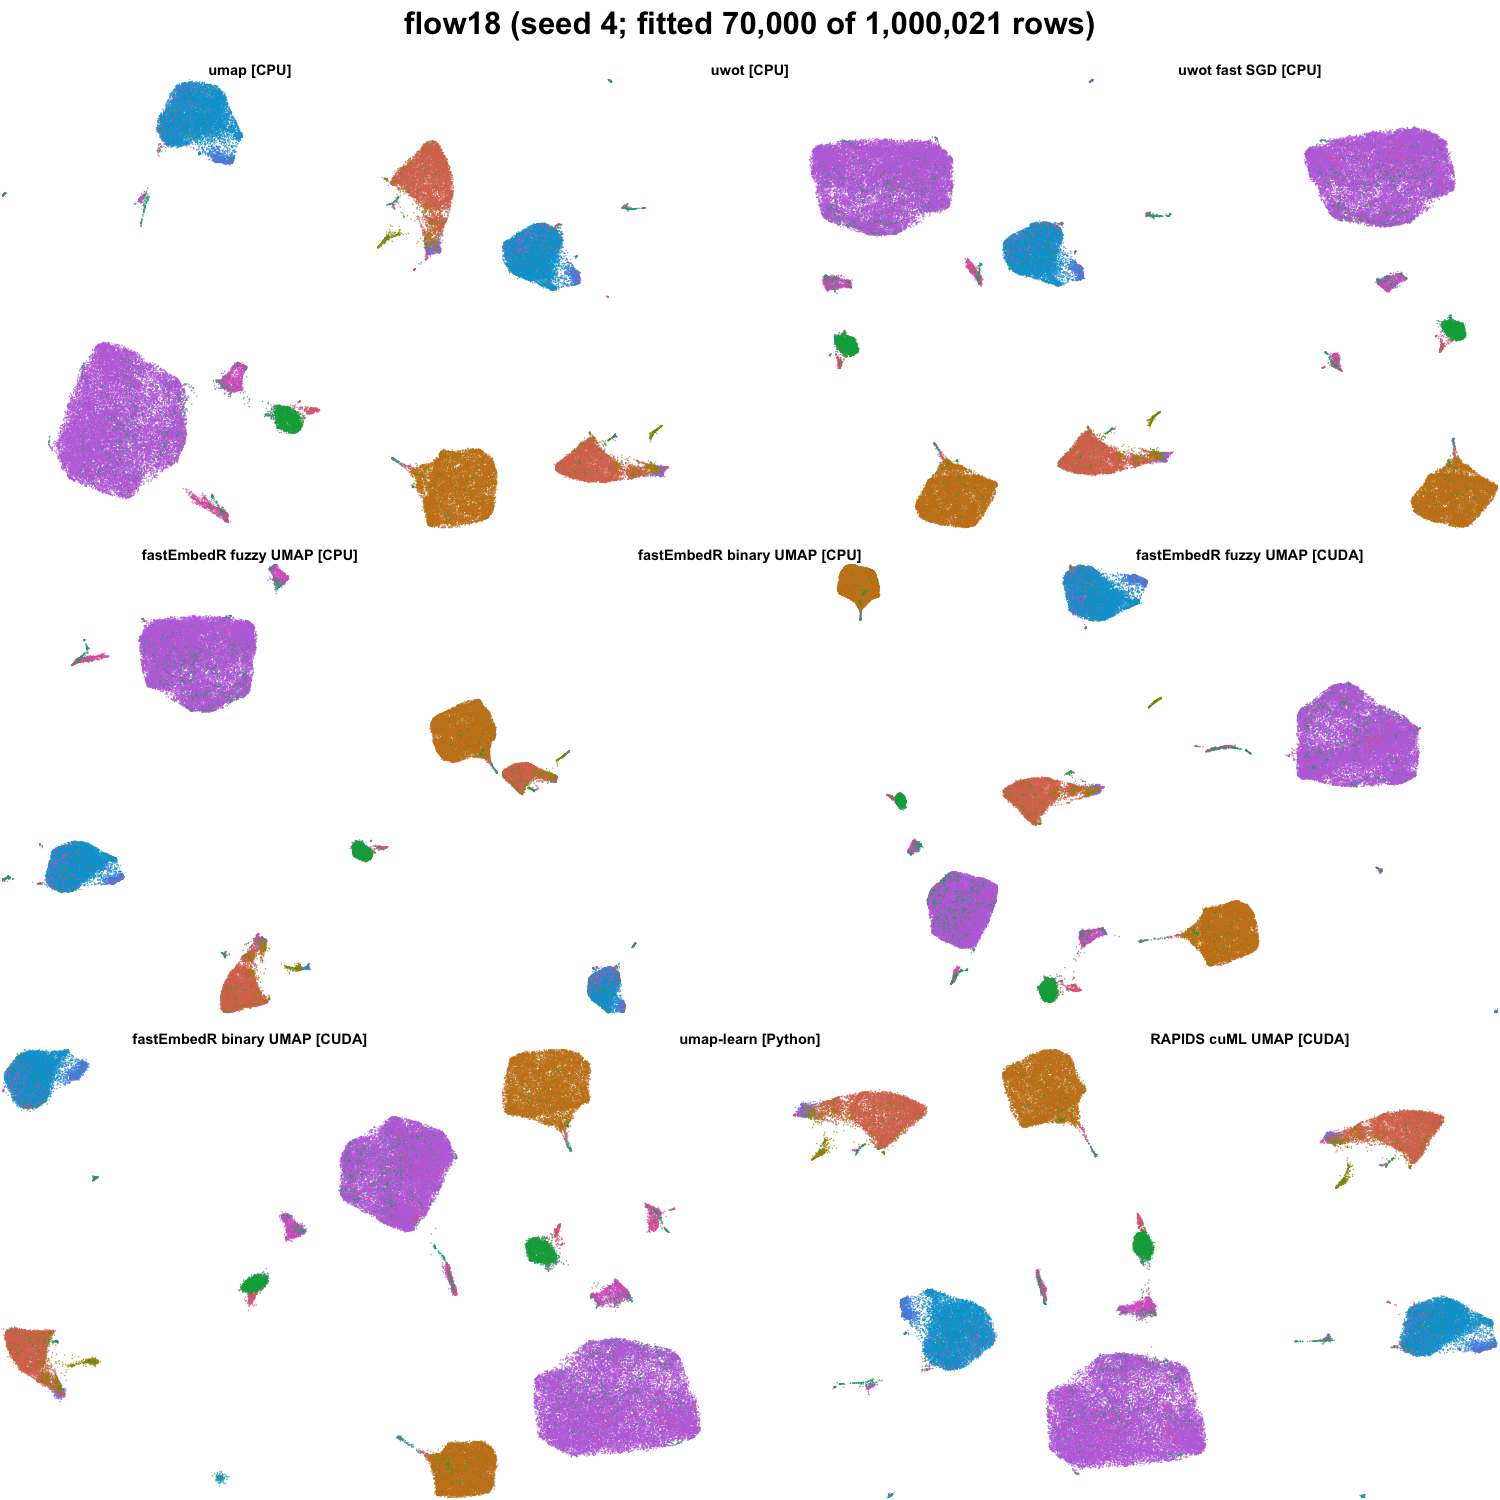
\includegraphics[width=0.94\textwidth]{figures/embedding_all_methods/flow18_umap.png}
\caption{flow18 UMAP outputs for the tested methods (seed 4; fitted 70,000 of 1,000,021 rows). Colors encode benchmark labels and were not used for fitting.}
\end{figure}
\clearpage

\begin{figure}[p]
\centering
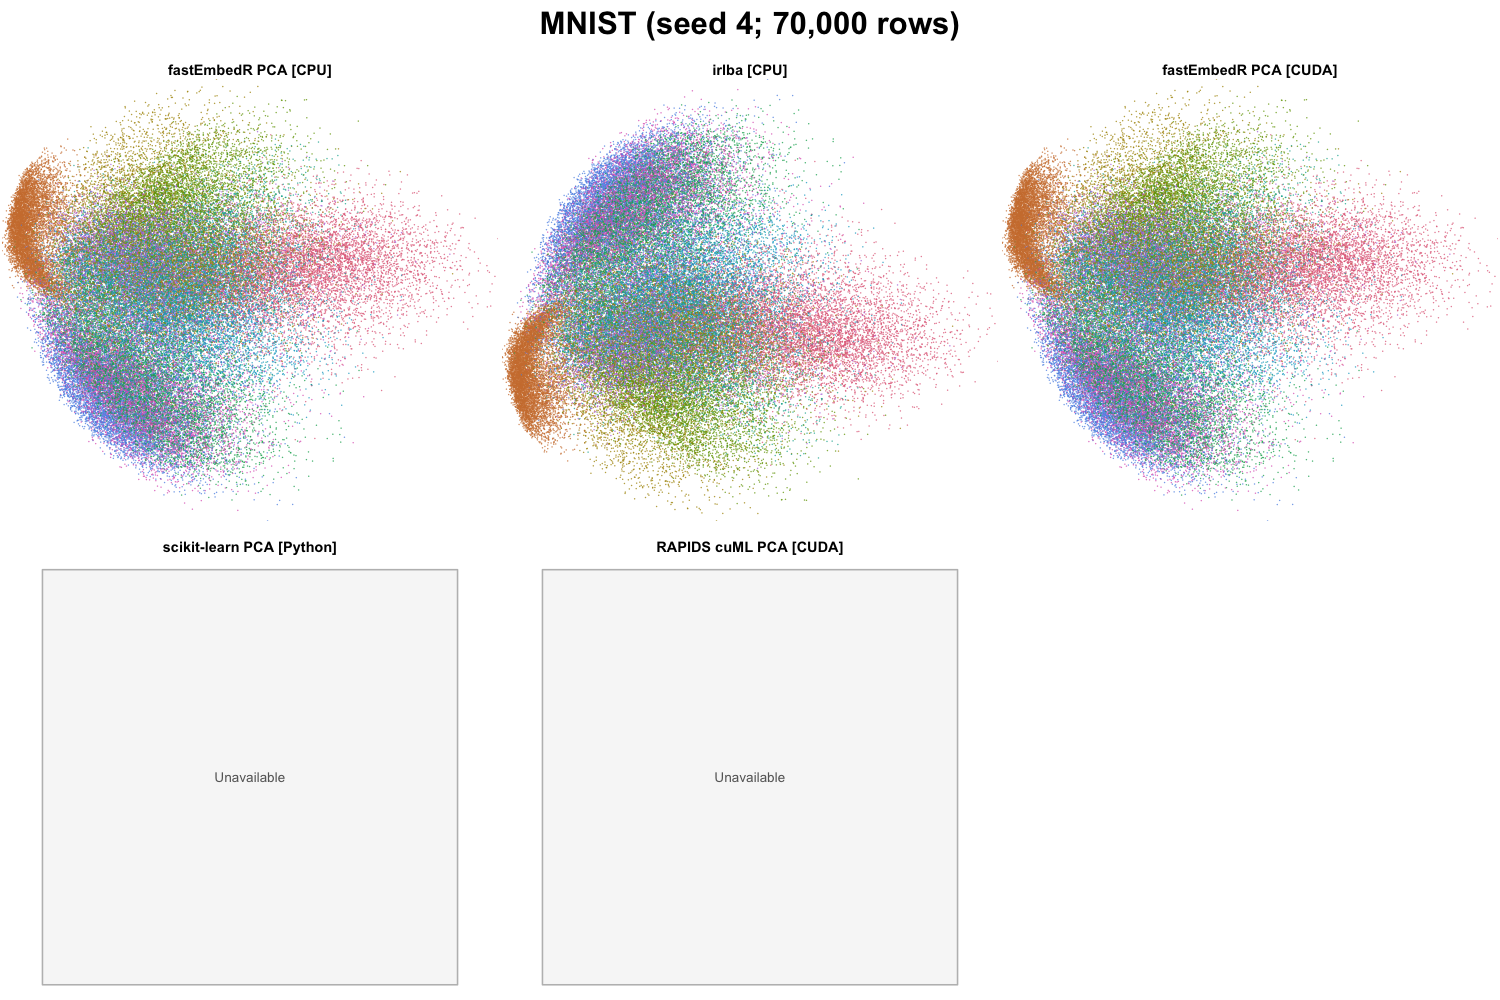
\includegraphics[width=0.94\textwidth]{figures/embedding_all_methods/MNIST_pca.png}
\caption{MNIST PCA outputs for the tested methods (seed 4; 70,000 rows). Colors encode benchmark labels and were not used for fitting.}
\end{figure}
\clearpage

\begin{figure}[p]
\centering
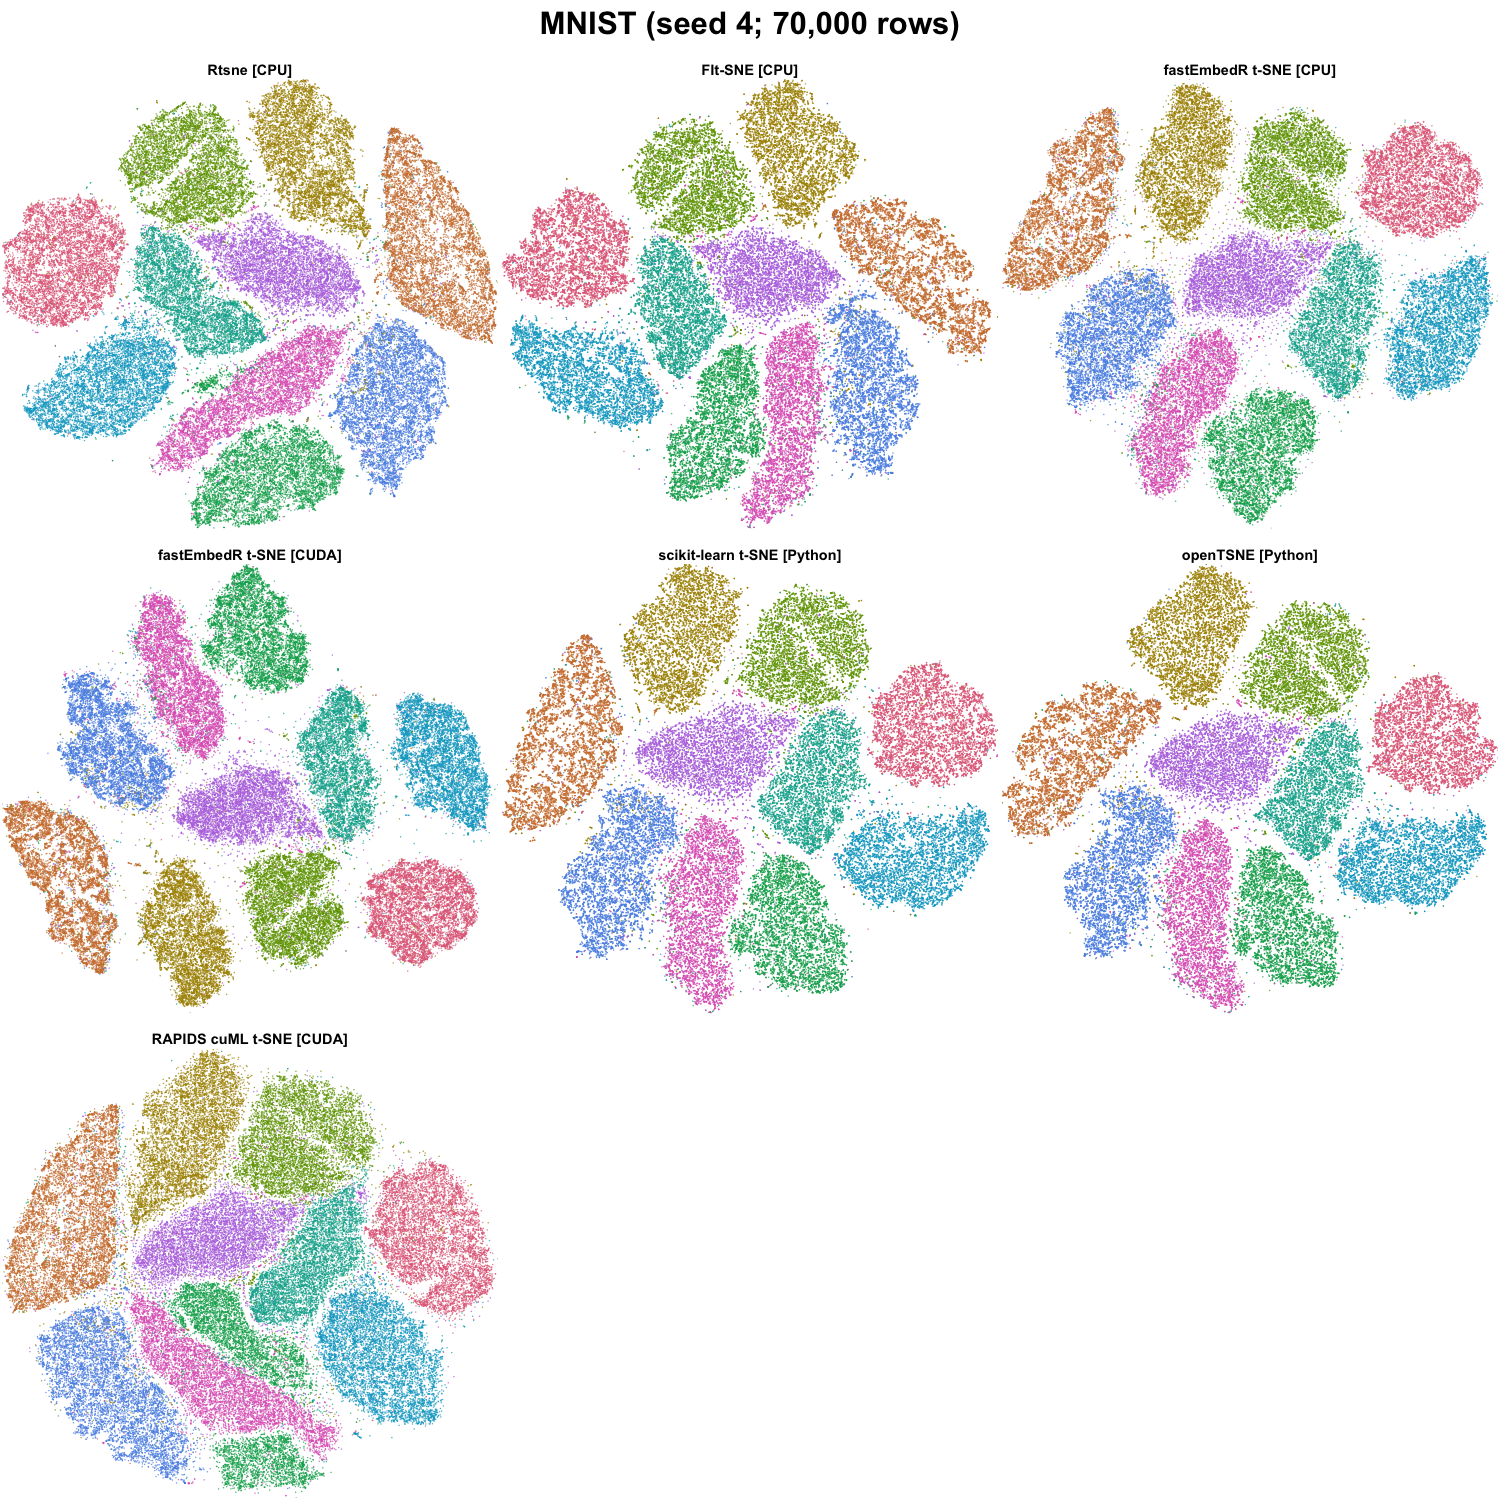
\includegraphics[width=0.94\textwidth]{figures/embedding_all_methods/MNIST_tsne.png}
\caption{MNIST t-SNE outputs for the tested methods (seed 4; 70,000 rows). Colors encode benchmark labels and were not used for fitting.}
\end{figure}
\clearpage

\begin{figure}[p]
\centering
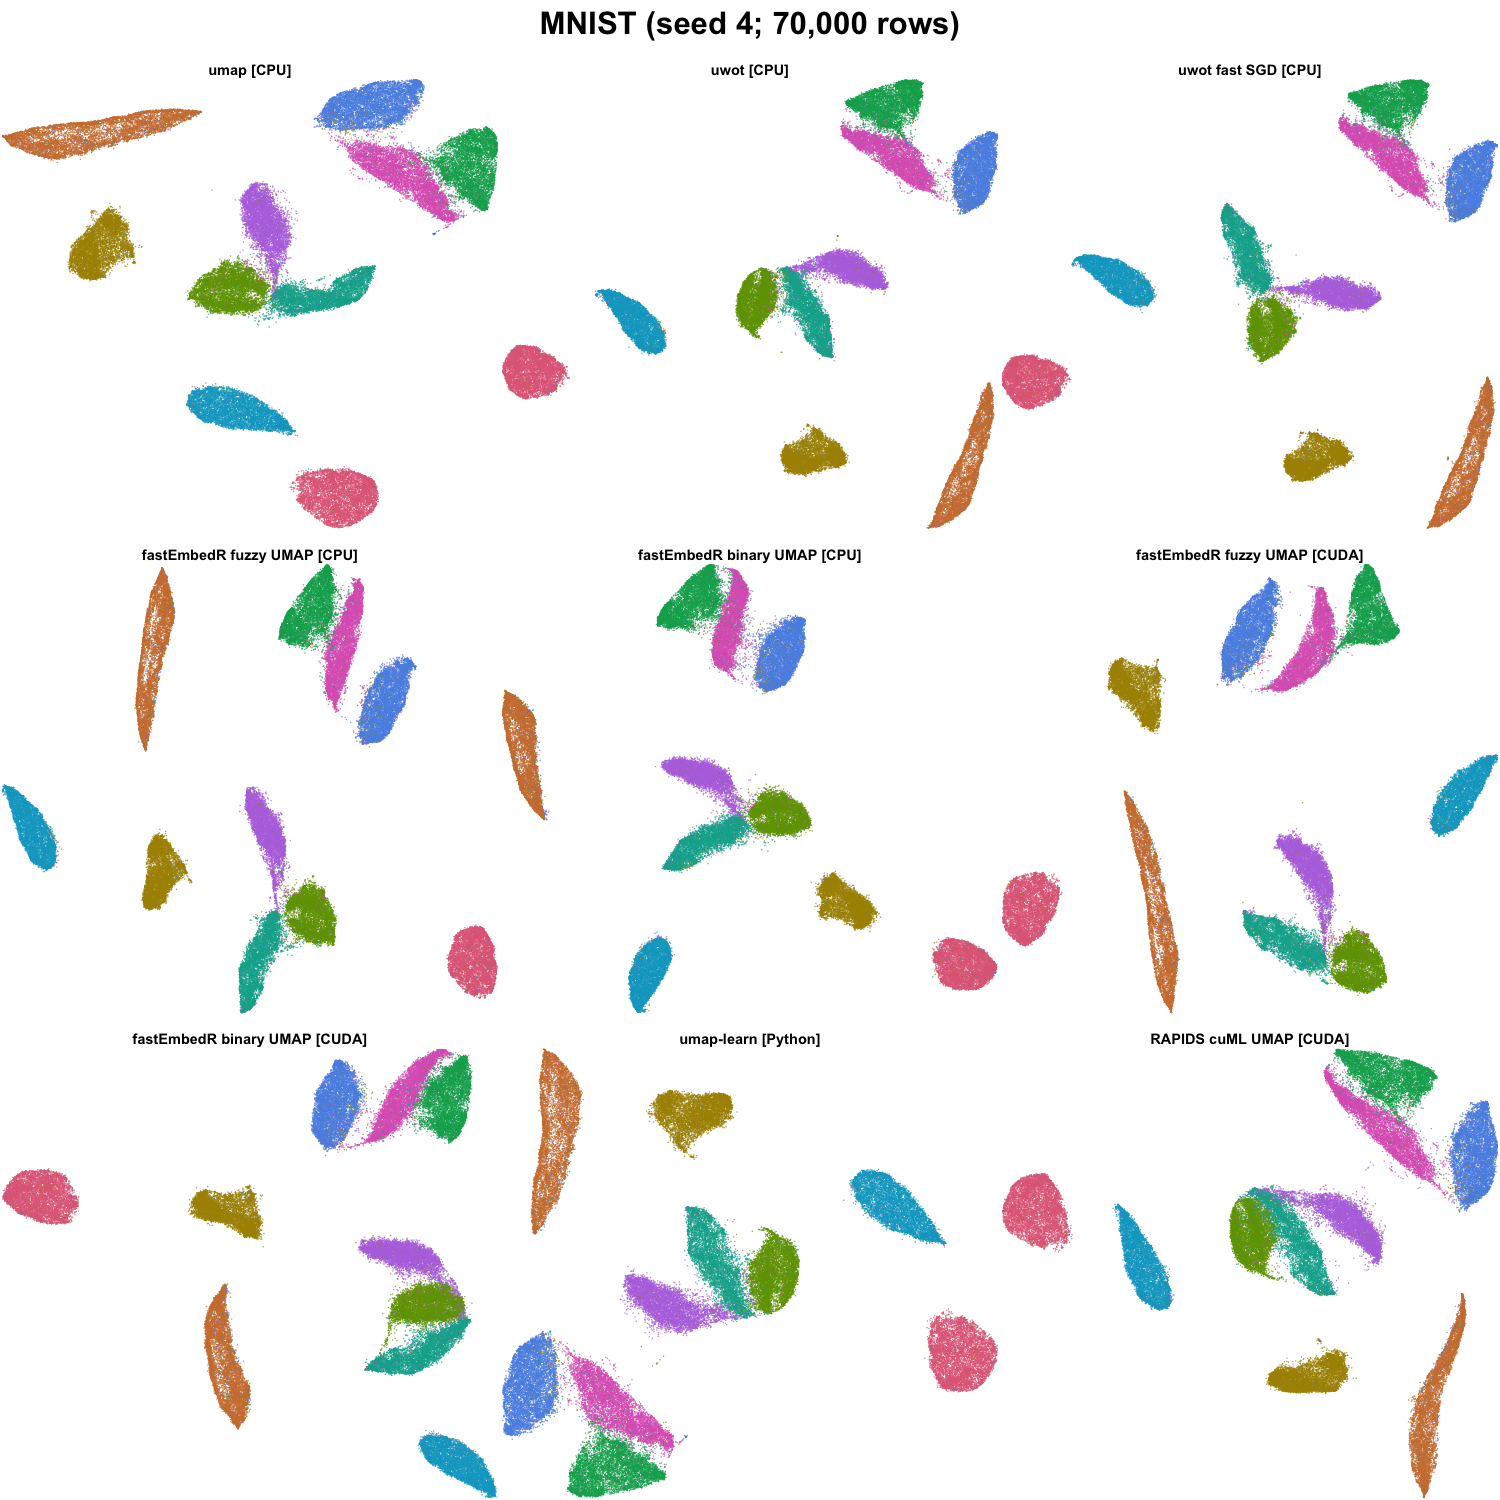
\includegraphics[width=0.94\textwidth]{figures/embedding_all_methods/MNIST_umap.png}
\caption{MNIST UMAP outputs for the tested methods (seed 4; 70,000 rows). Colors encode benchmark labels and were not used for fitting.}
\end{figure}
\clearpage

\begin{figure}[p]
\centering
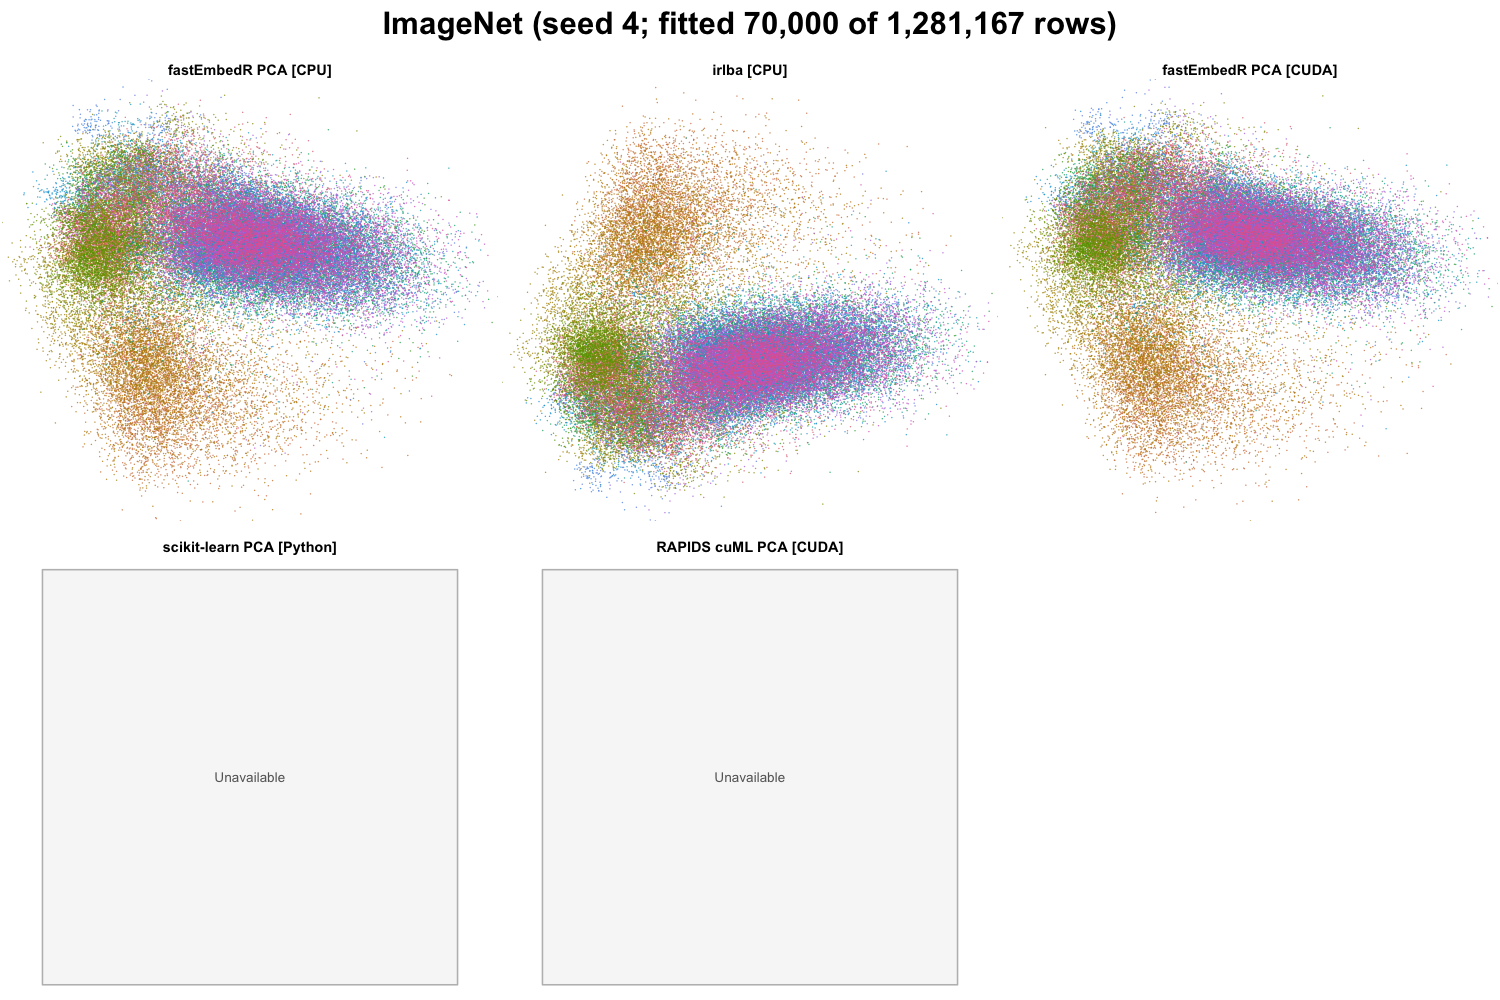
\includegraphics[width=0.94\textwidth]{figures/embedding_all_methods/imagenet_pca.png}
\caption{ImageNet PCA outputs for the tested methods (seed 4; fitted 70,000 of 1,281,167 rows). Colors encode benchmark labels and were not used for fitting.}
\end{figure}
\clearpage

\begin{figure}[p]
\centering
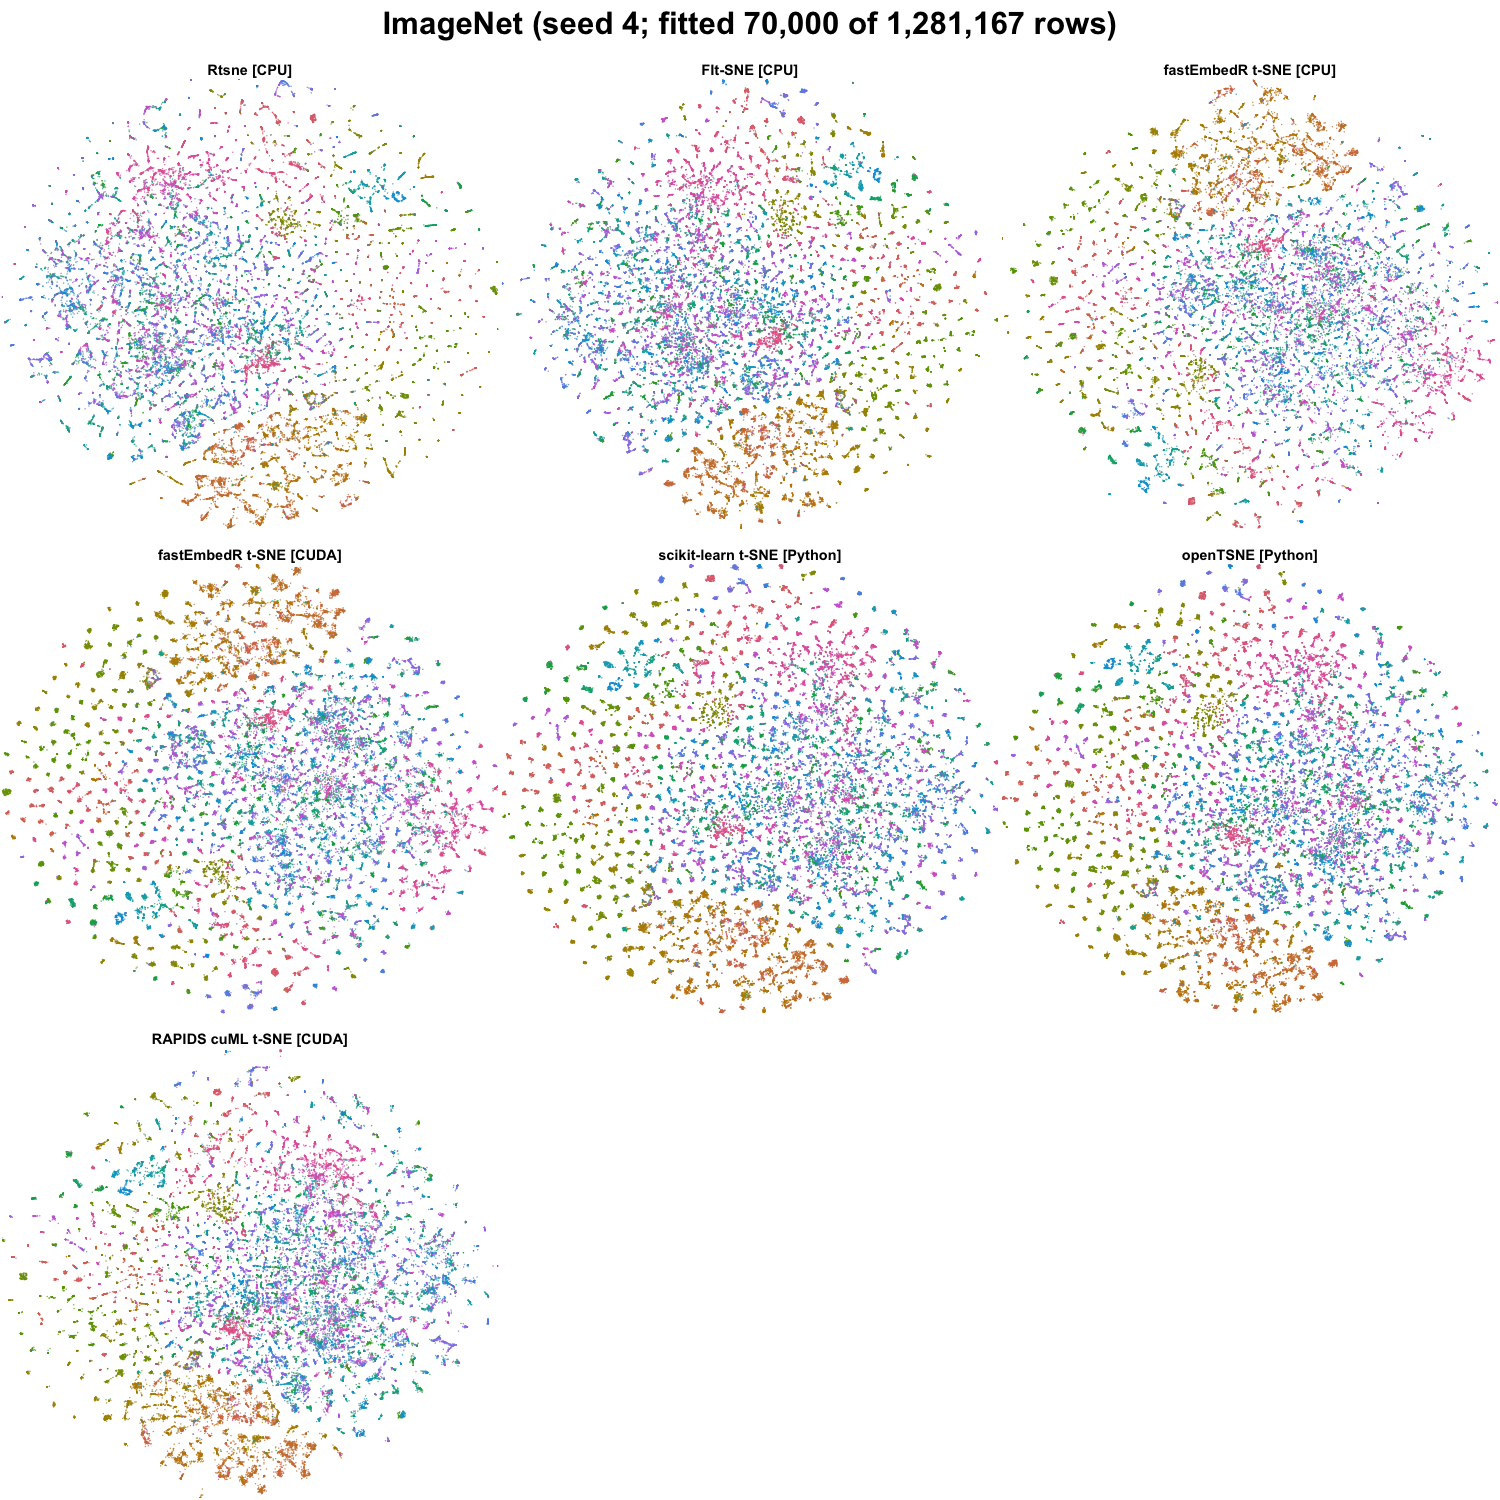
\includegraphics[width=0.94\textwidth]{figures/embedding_all_methods/imagenet_tsne.png}
\caption{ImageNet t-SNE outputs for the tested methods (seed 4; fitted 70,000 of 1,281,167 rows). Colors encode benchmark labels and were not used for fitting.}
\end{figure}
\clearpage

\begin{figure}[p]
\centering
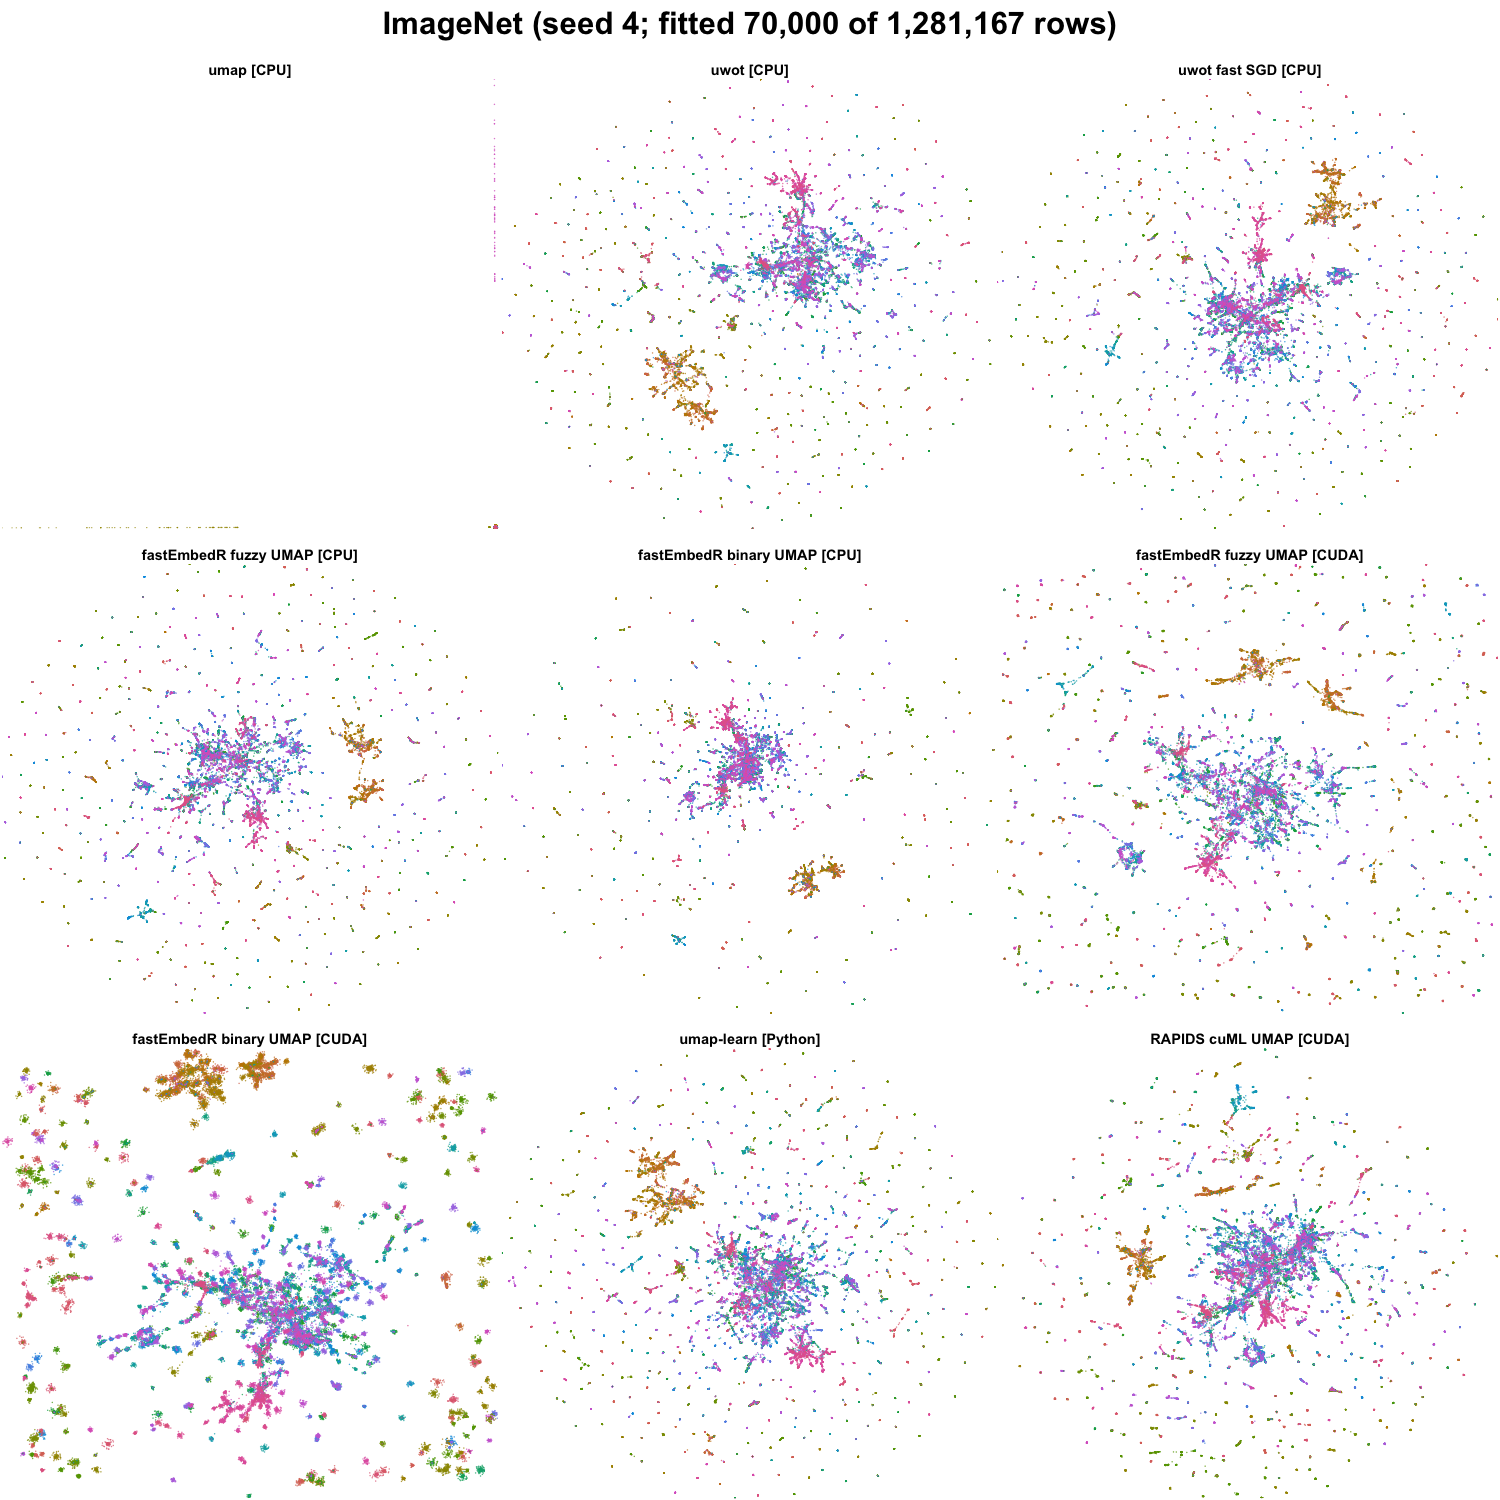
\includegraphics[width=0.94\textwidth]{figures/embedding_all_methods/imagenet_umap.png}
\caption{ImageNet UMAP outputs for the tested methods (seed 4; fitted 70,000 of 1,281,167 rows). Colors encode benchmark labels and were not used for fitting.}
\end{figure}
\clearpage

\begin{figure}[p]
\centering
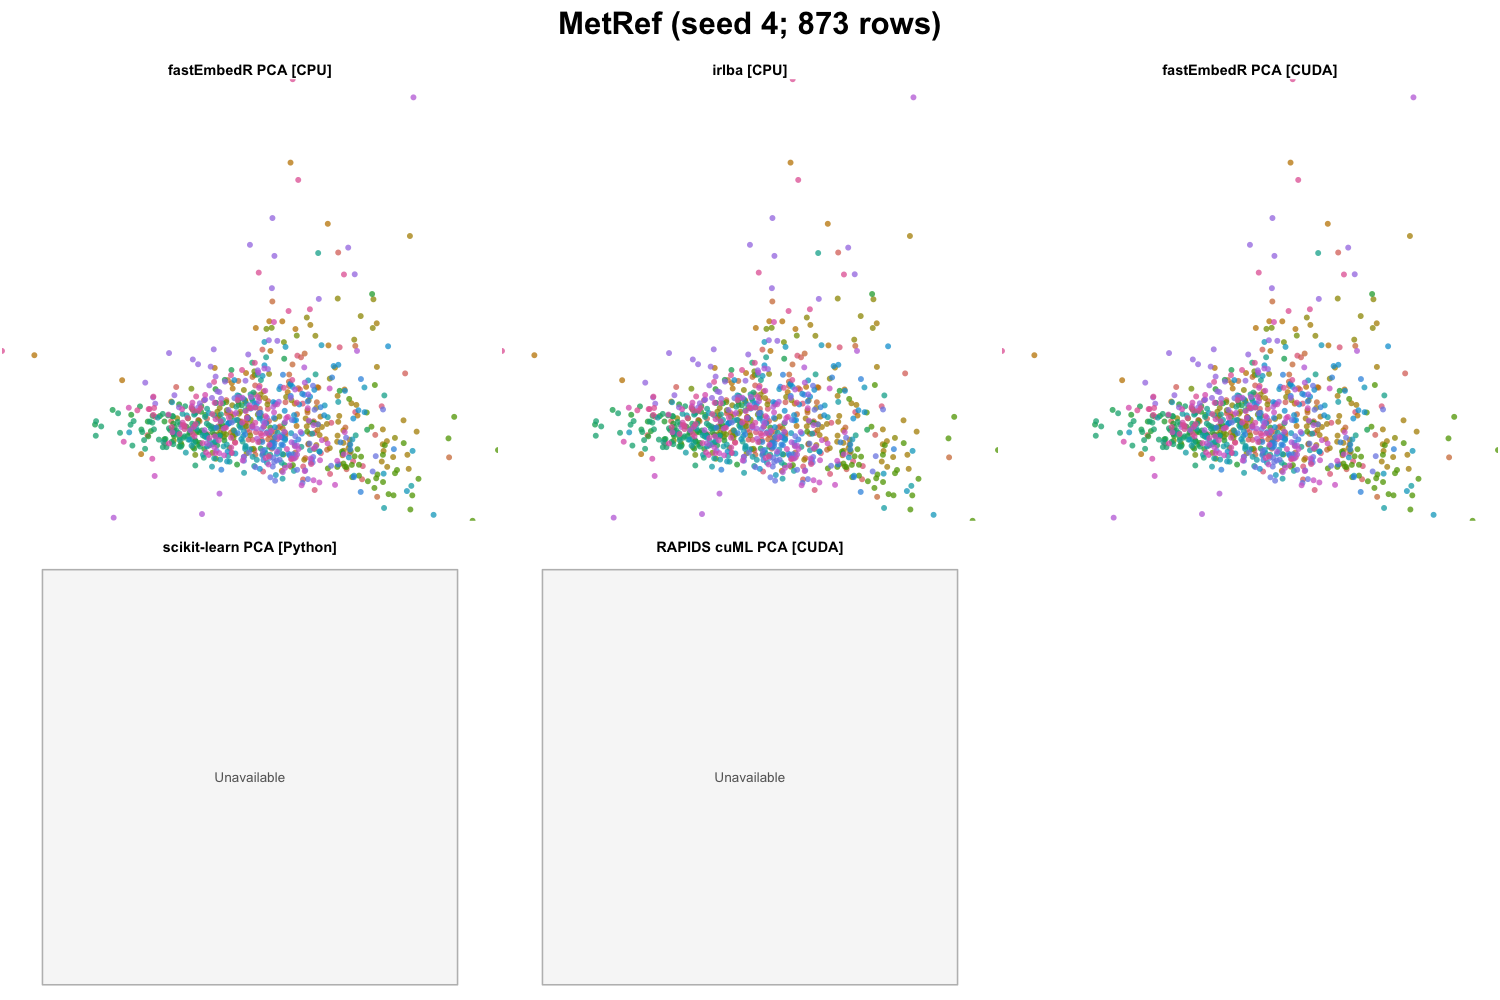
\includegraphics[width=0.94\textwidth]{figures/embedding_all_methods/MetRef_pca.png}
\caption{MetRef PCA outputs for the tested methods (seed 4; 873 rows). Colors encode benchmark labels and were not used for fitting.}
\end{figure}
\clearpage

\begin{figure}[p]
\centering
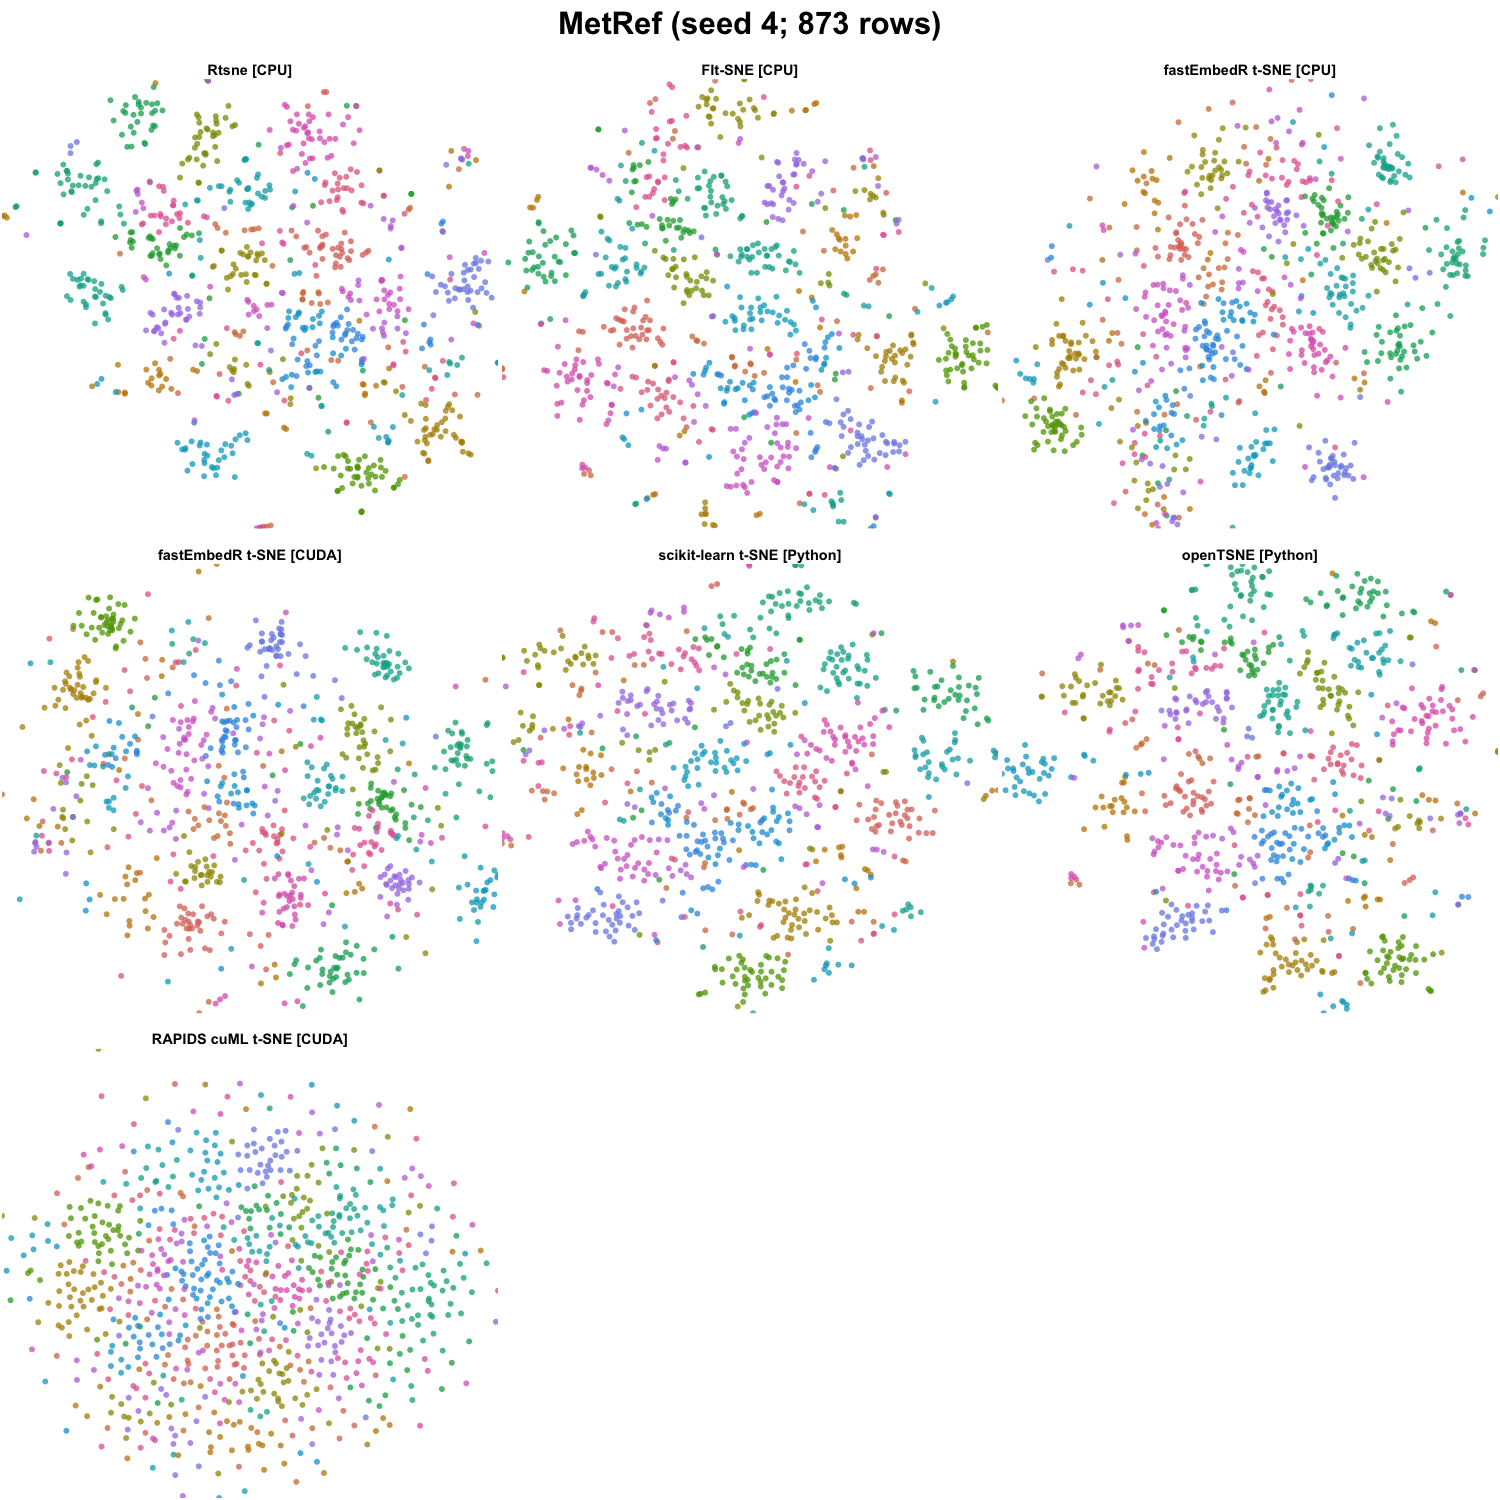
\includegraphics[width=0.94\textwidth]{figures/embedding_all_methods/MetRef_tsne.png}
\caption{MetRef t-SNE outputs for the tested methods (seed 4; 873 rows). Colors encode benchmark labels and were not used for fitting.}
\end{figure}
\clearpage

\begin{figure}[p]
\centering
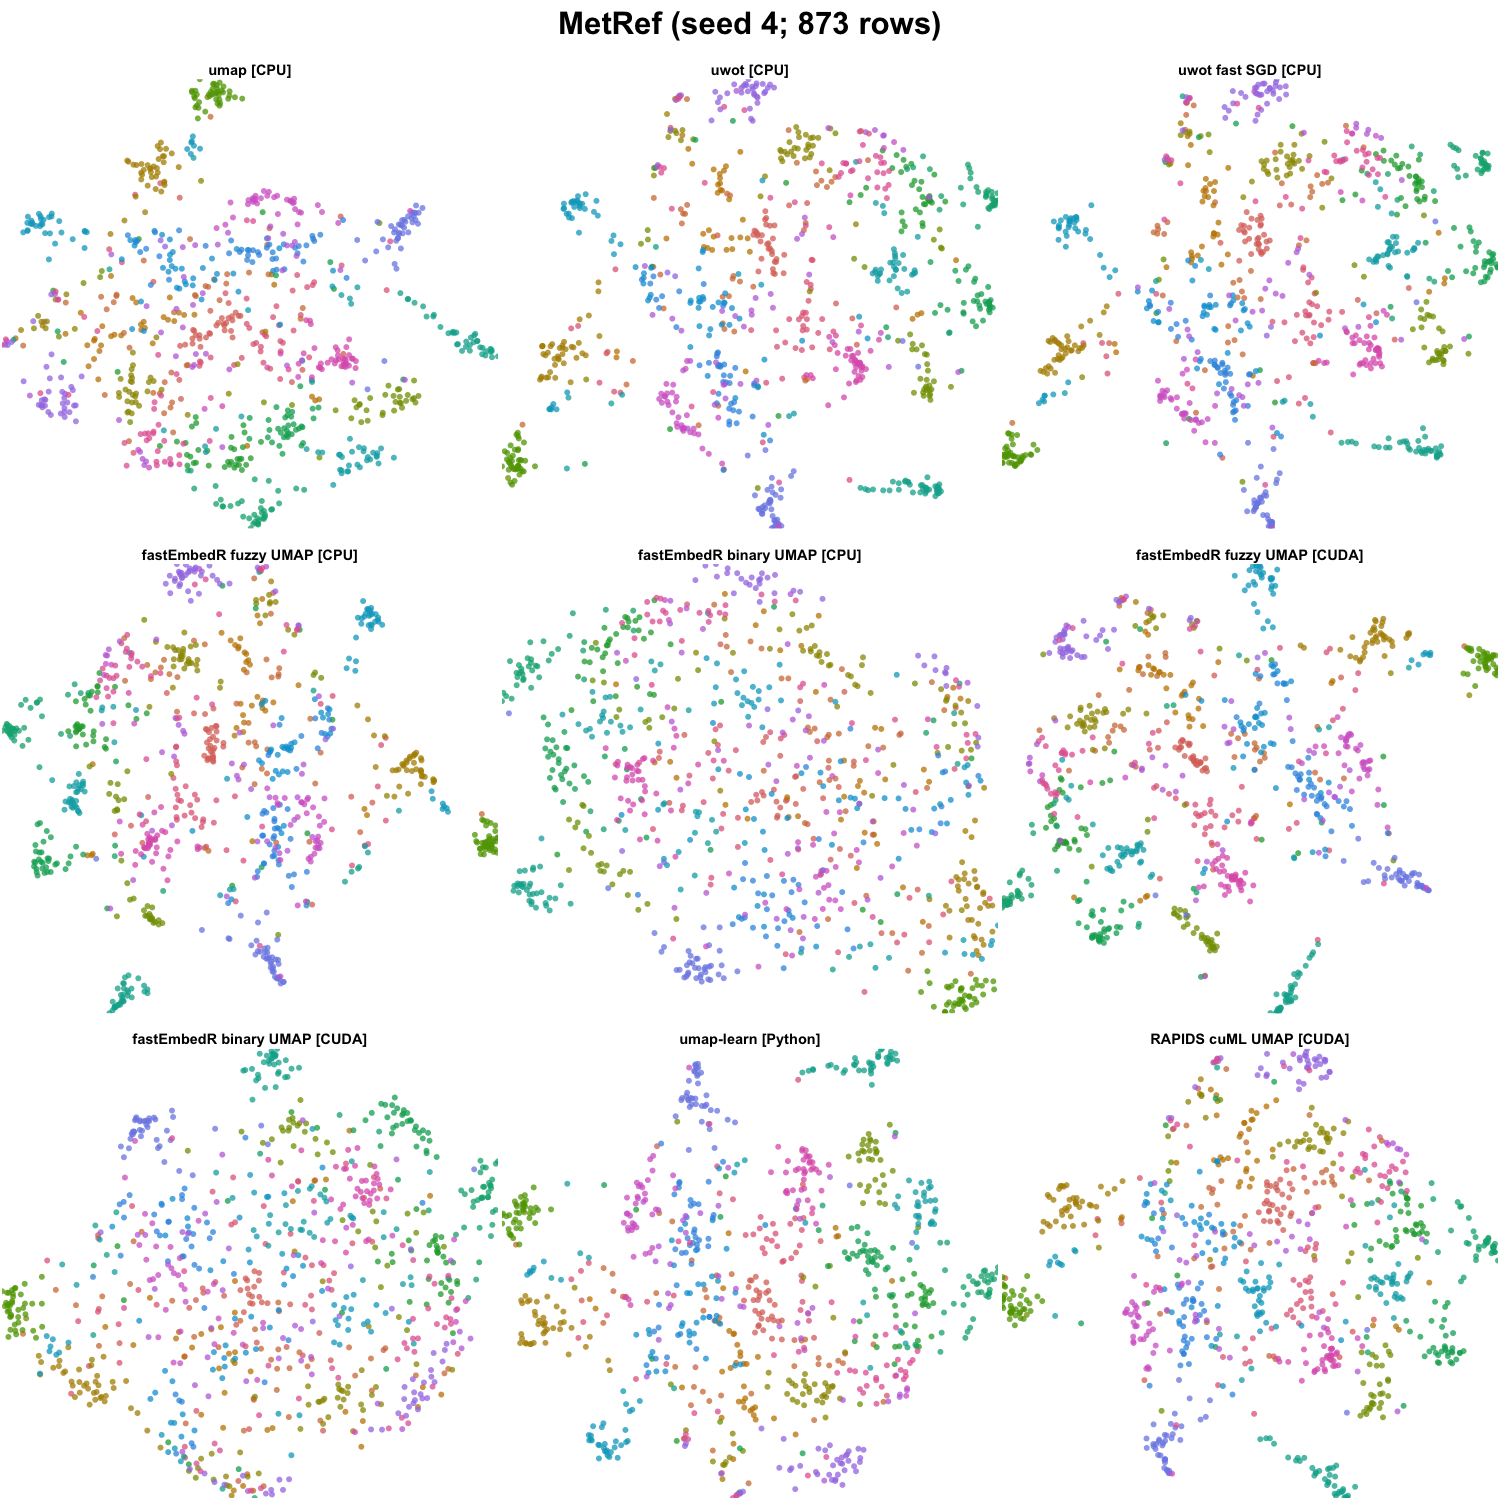
\includegraphics[width=0.94\textwidth]{figures/embedding_all_methods/MetRef_umap.png}
\caption{MetRef UMAP outputs for the tested methods (seed 4; 873 rows). Colors encode benchmark labels and were not used for fitting.}
\end{figure}
\clearpage

\begin{figure}[p]
\centering
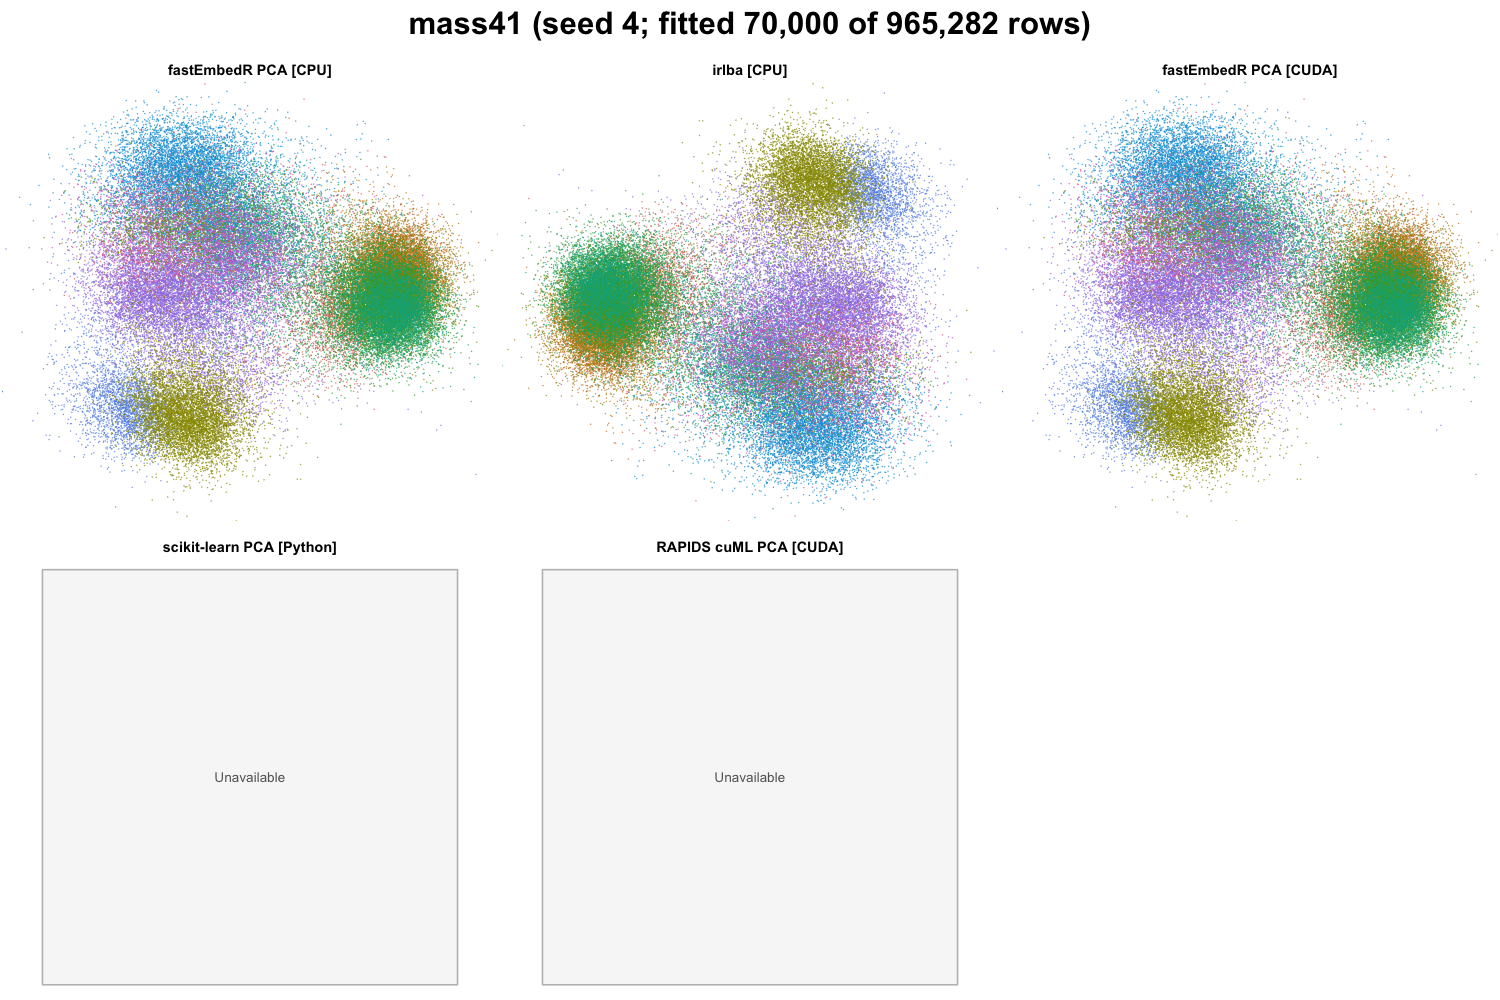
\includegraphics[width=0.94\textwidth]{figures/embedding_all_methods/mass41_pca.png}
\caption{mass41 PCA outputs for the tested methods (seed 4; fitted 70,000 of 965,282 rows). Colors encode benchmark labels and were not used for fitting.}
\end{figure}
\clearpage

\begin{figure}[p]
\centering
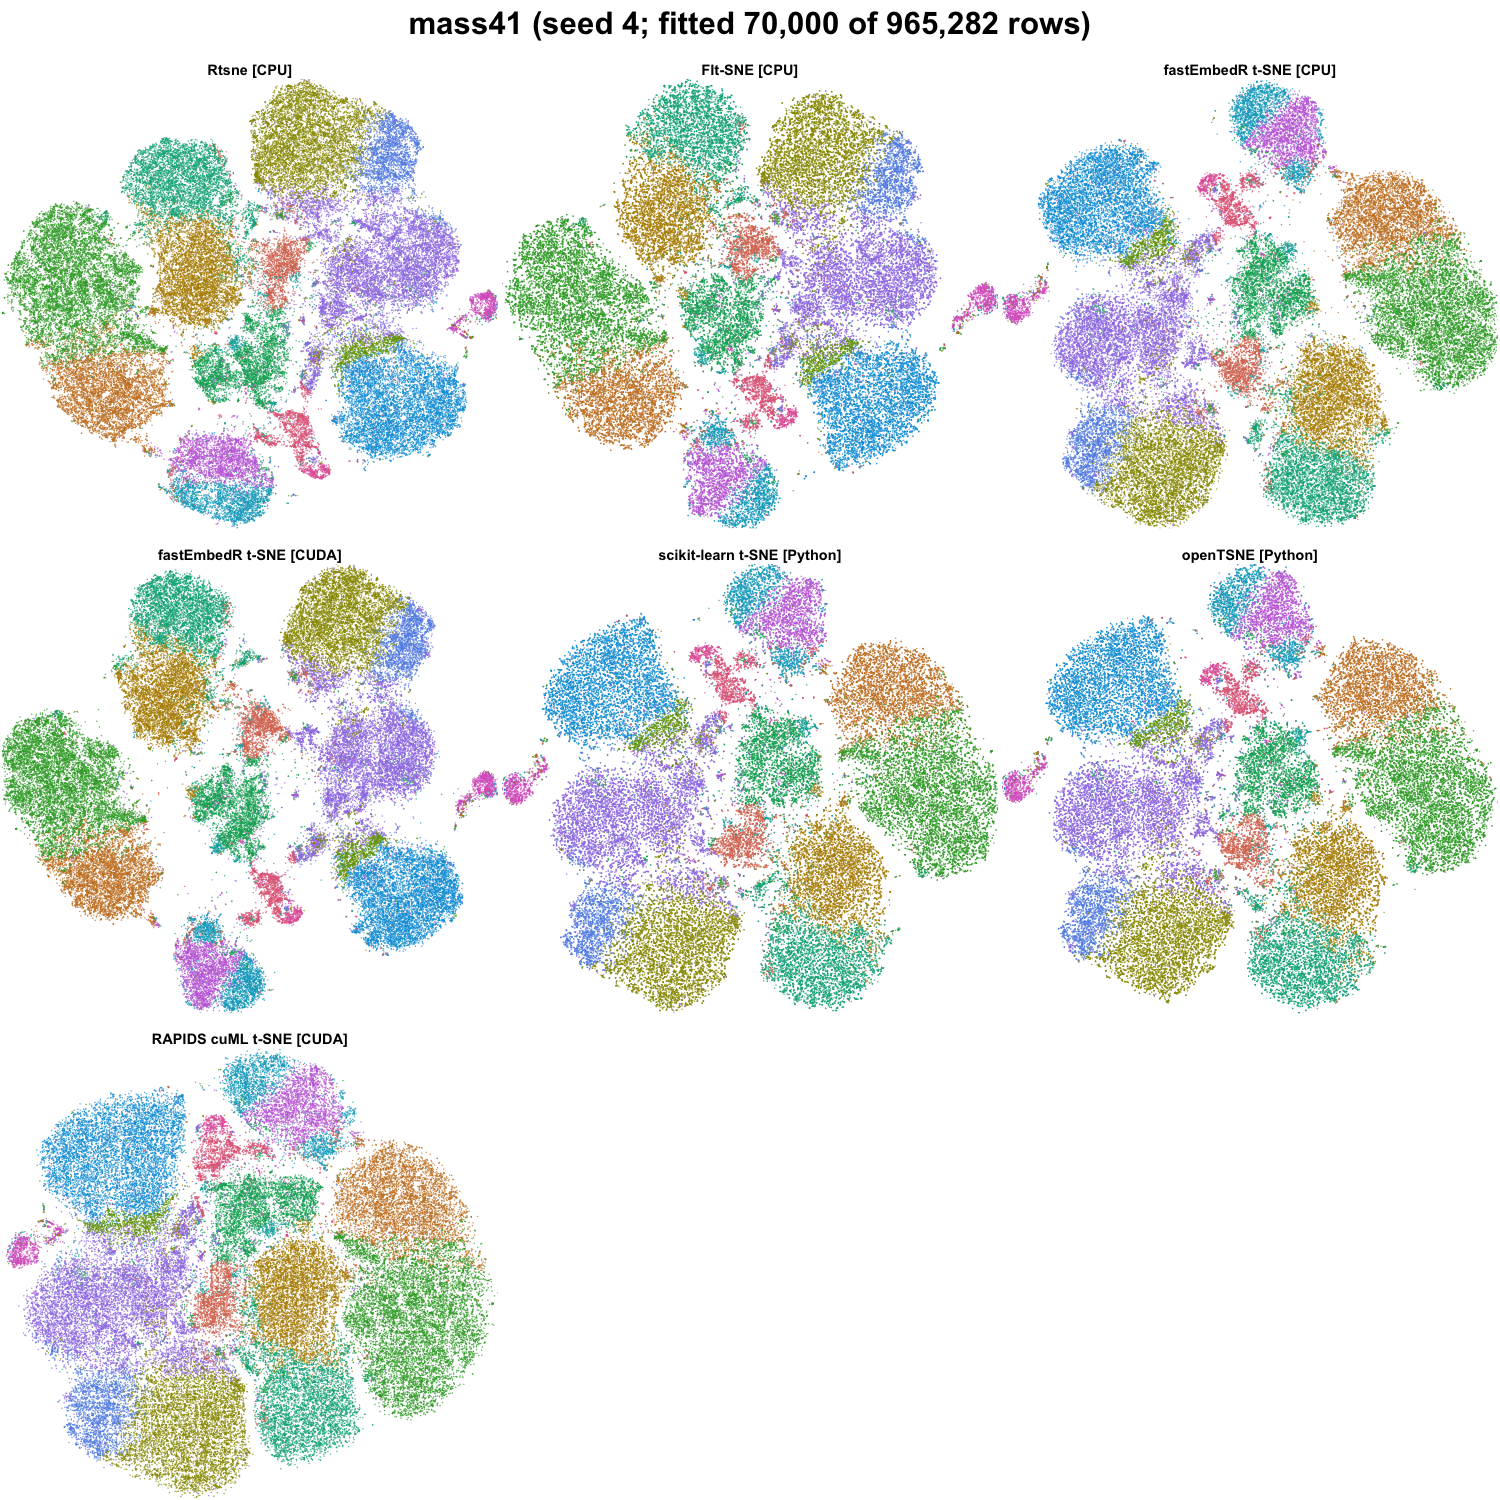
\includegraphics[width=0.94\textwidth]{figures/embedding_all_methods/mass41_tsne.png}
\caption{mass41 t-SNE outputs for the tested methods (seed 4; fitted 70,000 of 965,282 rows). Colors encode benchmark labels and were not used for fitting.}
\end{figure}
\clearpage

\begin{figure}[p]
\centering
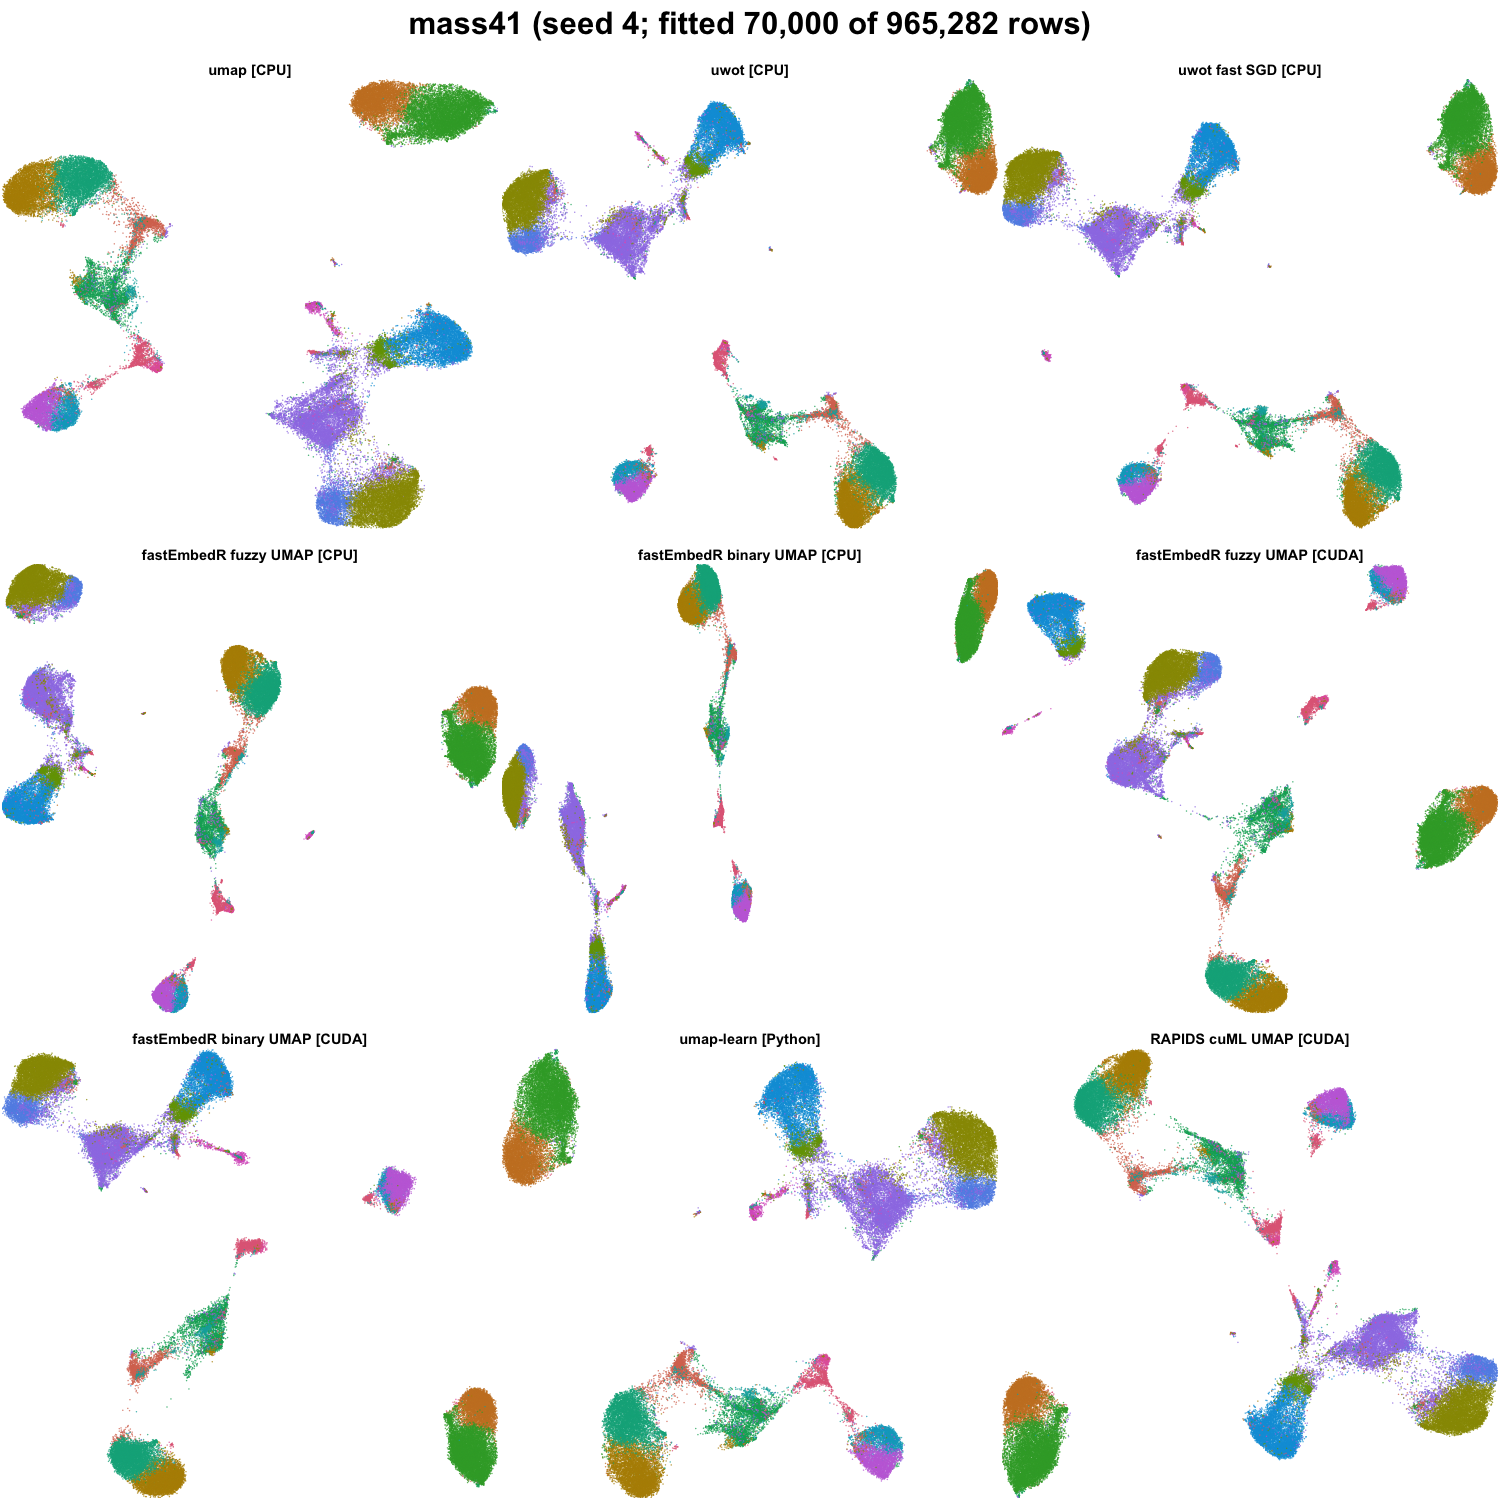
\includegraphics[width=0.94\textwidth]{figures/embedding_all_methods/mass41_umap.png}
\caption{mass41 UMAP outputs for the tested methods (seed 4; fitted 70,000 of 965,282 rows). Colors encode benchmark labels and were not used for fitting.}
\end{figure}
\clearpage

\begin{figure}[p]
\centering
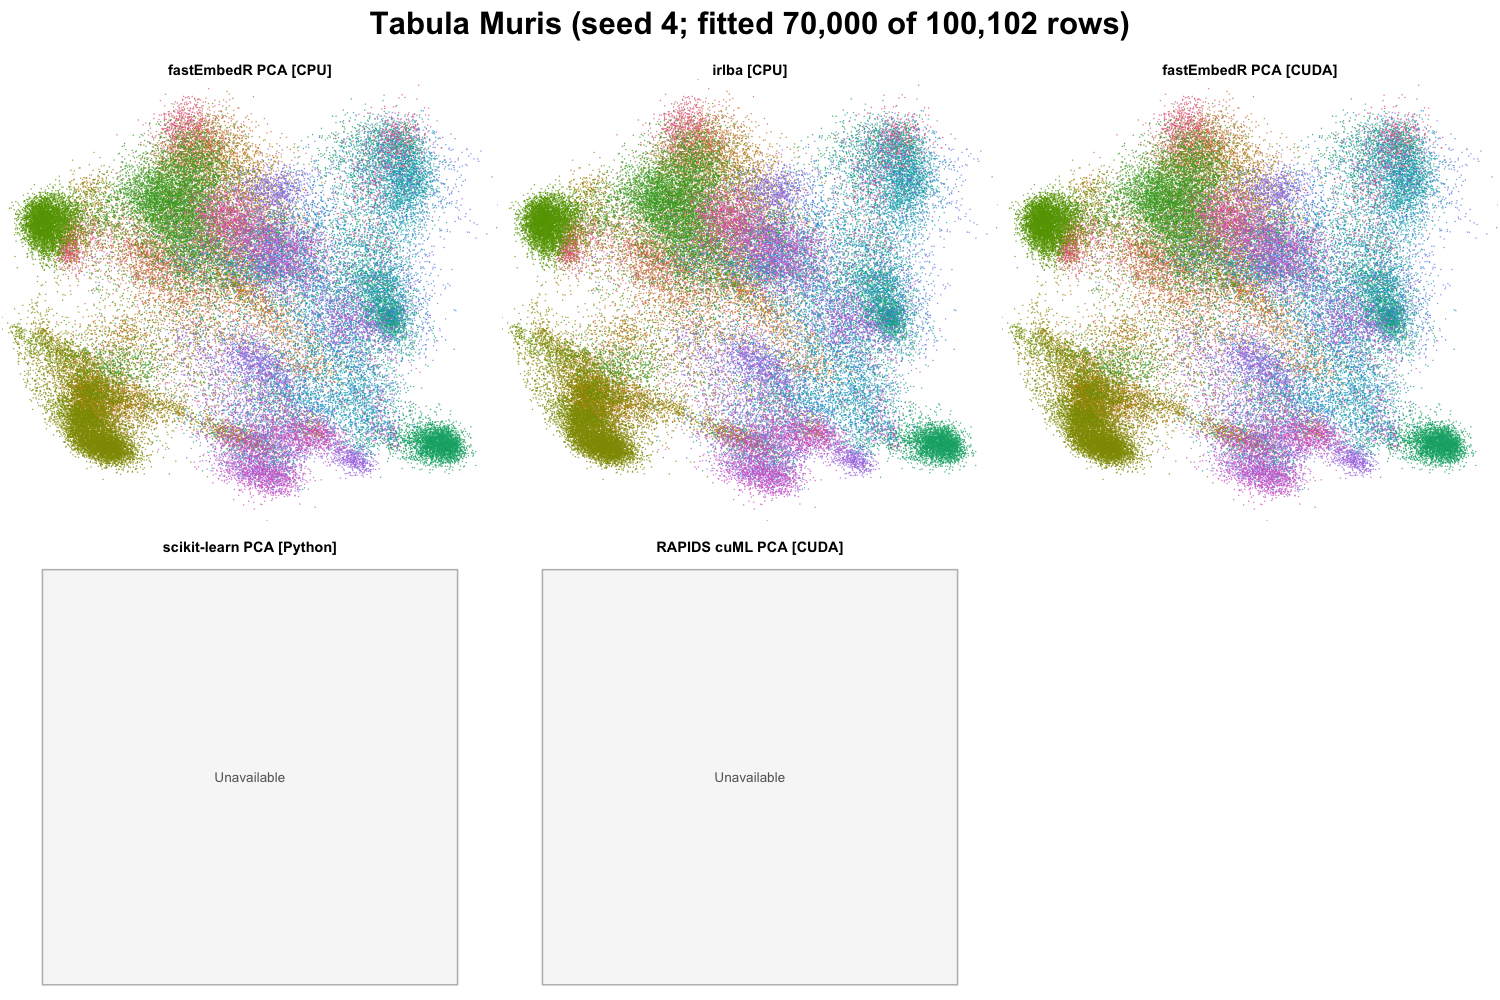
\includegraphics[width=0.94\textwidth]{figures/embedding_all_methods/TabulaMuris_pca.png}
\caption{Tabula Muris PCA outputs for the tested methods (seed 4; fitted 70,000 of 100,102 rows). Colors encode benchmark labels and were not used for fitting.}
\end{figure}
\clearpage

\begin{figure}[p]
\centering
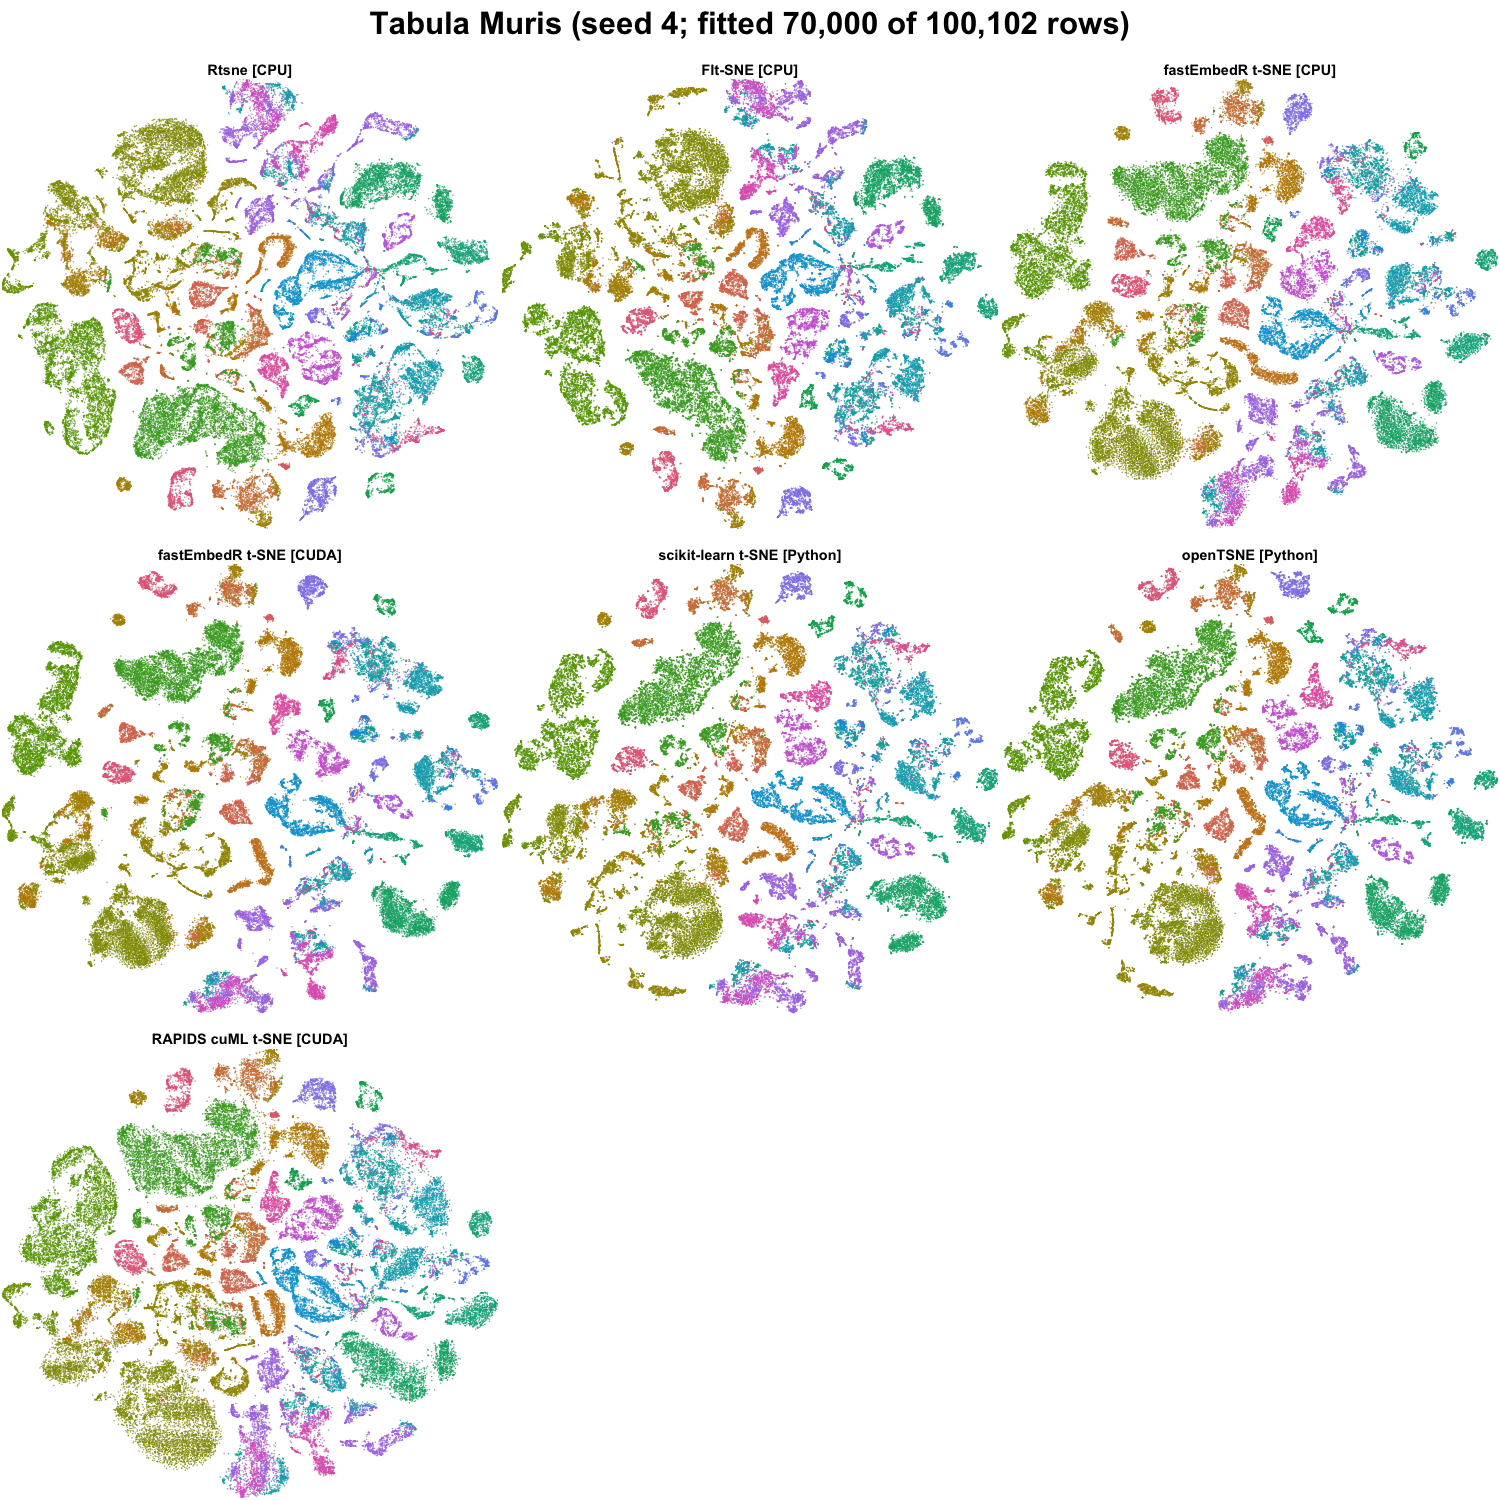
\includegraphics[width=0.94\textwidth]{figures/embedding_all_methods/TabulaMuris_tsne.png}
\caption{Tabula Muris t-SNE outputs for the tested methods (seed 4; fitted 70,000 of 100,102 rows). Colors encode benchmark labels and were not used for fitting.}
\end{figure}
\clearpage

\begin{figure}[p]
\centering
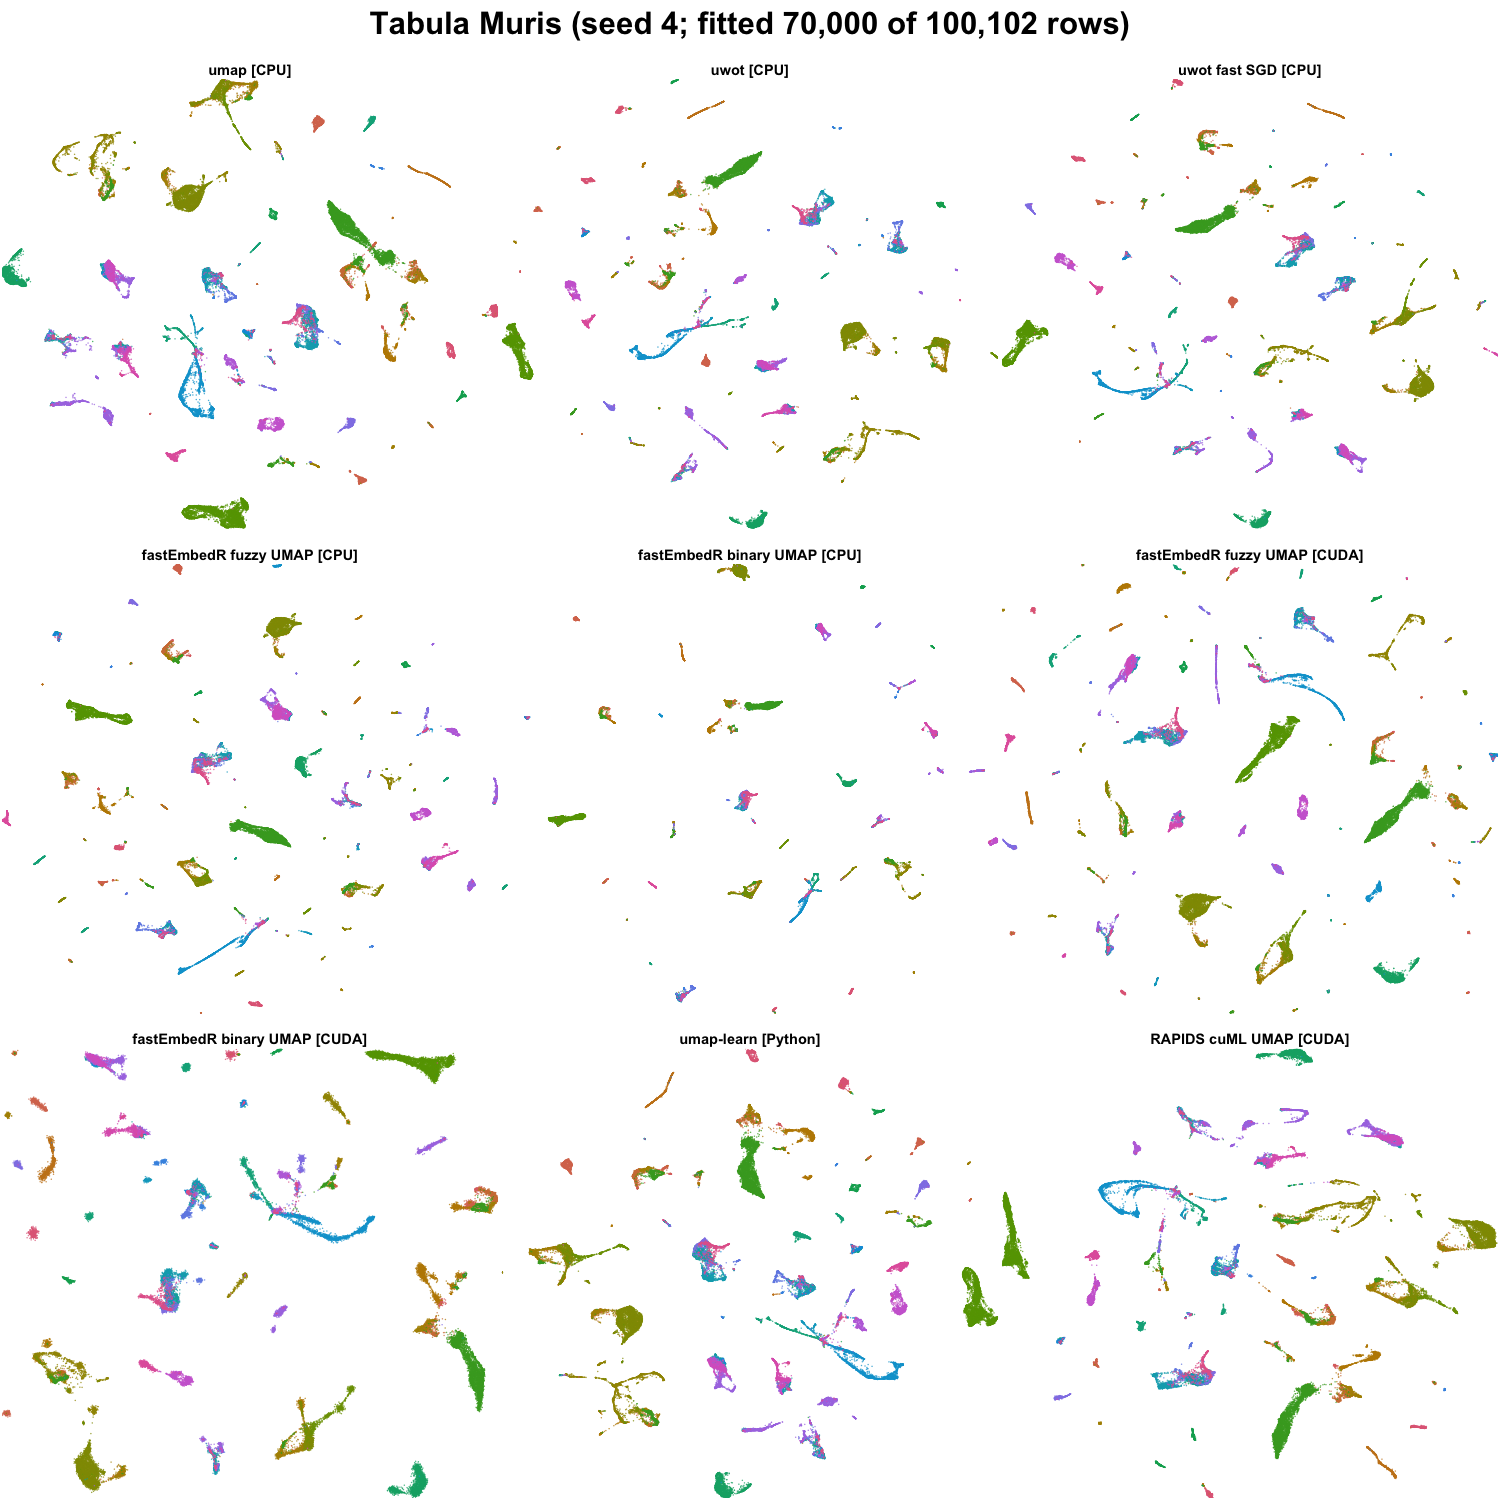
\includegraphics[width=0.94\textwidth]{figures/embedding_all_methods/TabulaMuris_umap.png}
\caption{Tabula Muris UMAP outputs for the tested methods (seed 4; fitted 70,000 of 100,102 rows). Colors encode benchmark labels and were not used for fitting.}
\end{figure}
\clearpage

\begin{figure}[p]
\centering
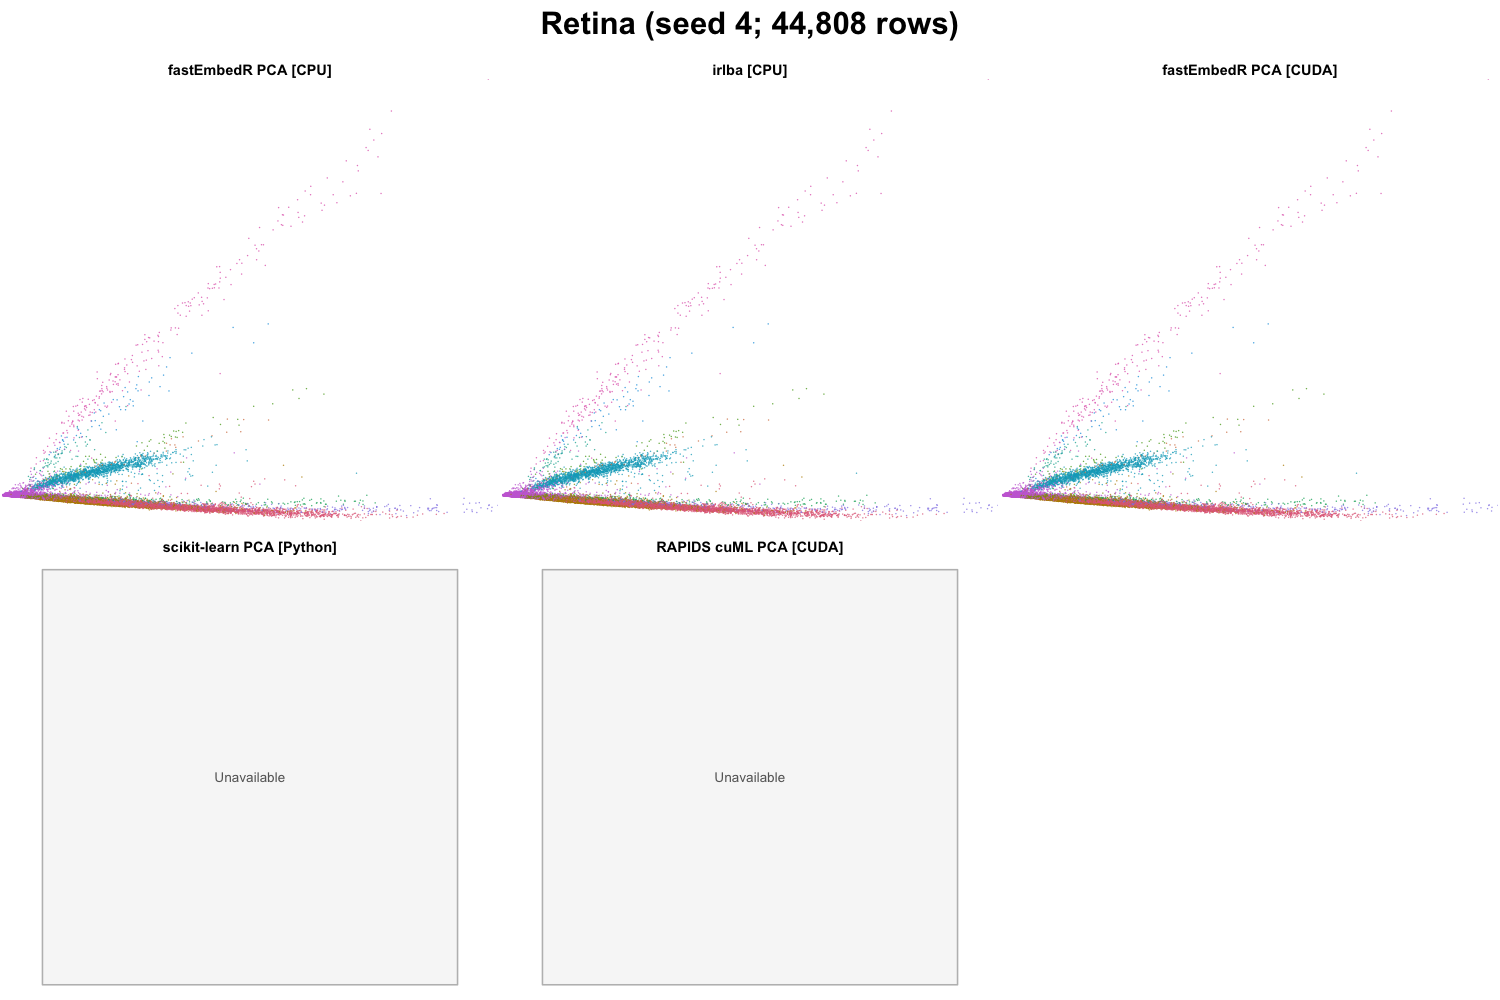
\includegraphics[width=0.94\textwidth]{figures/embedding_all_methods/Macosko2015_retina_pca.png}
\caption{Retina PCA outputs for the tested methods (seed 4; 44,808 rows). Colors encode benchmark labels and were not used for fitting.}
\end{figure}
\clearpage

\begin{figure}[p]
\centering
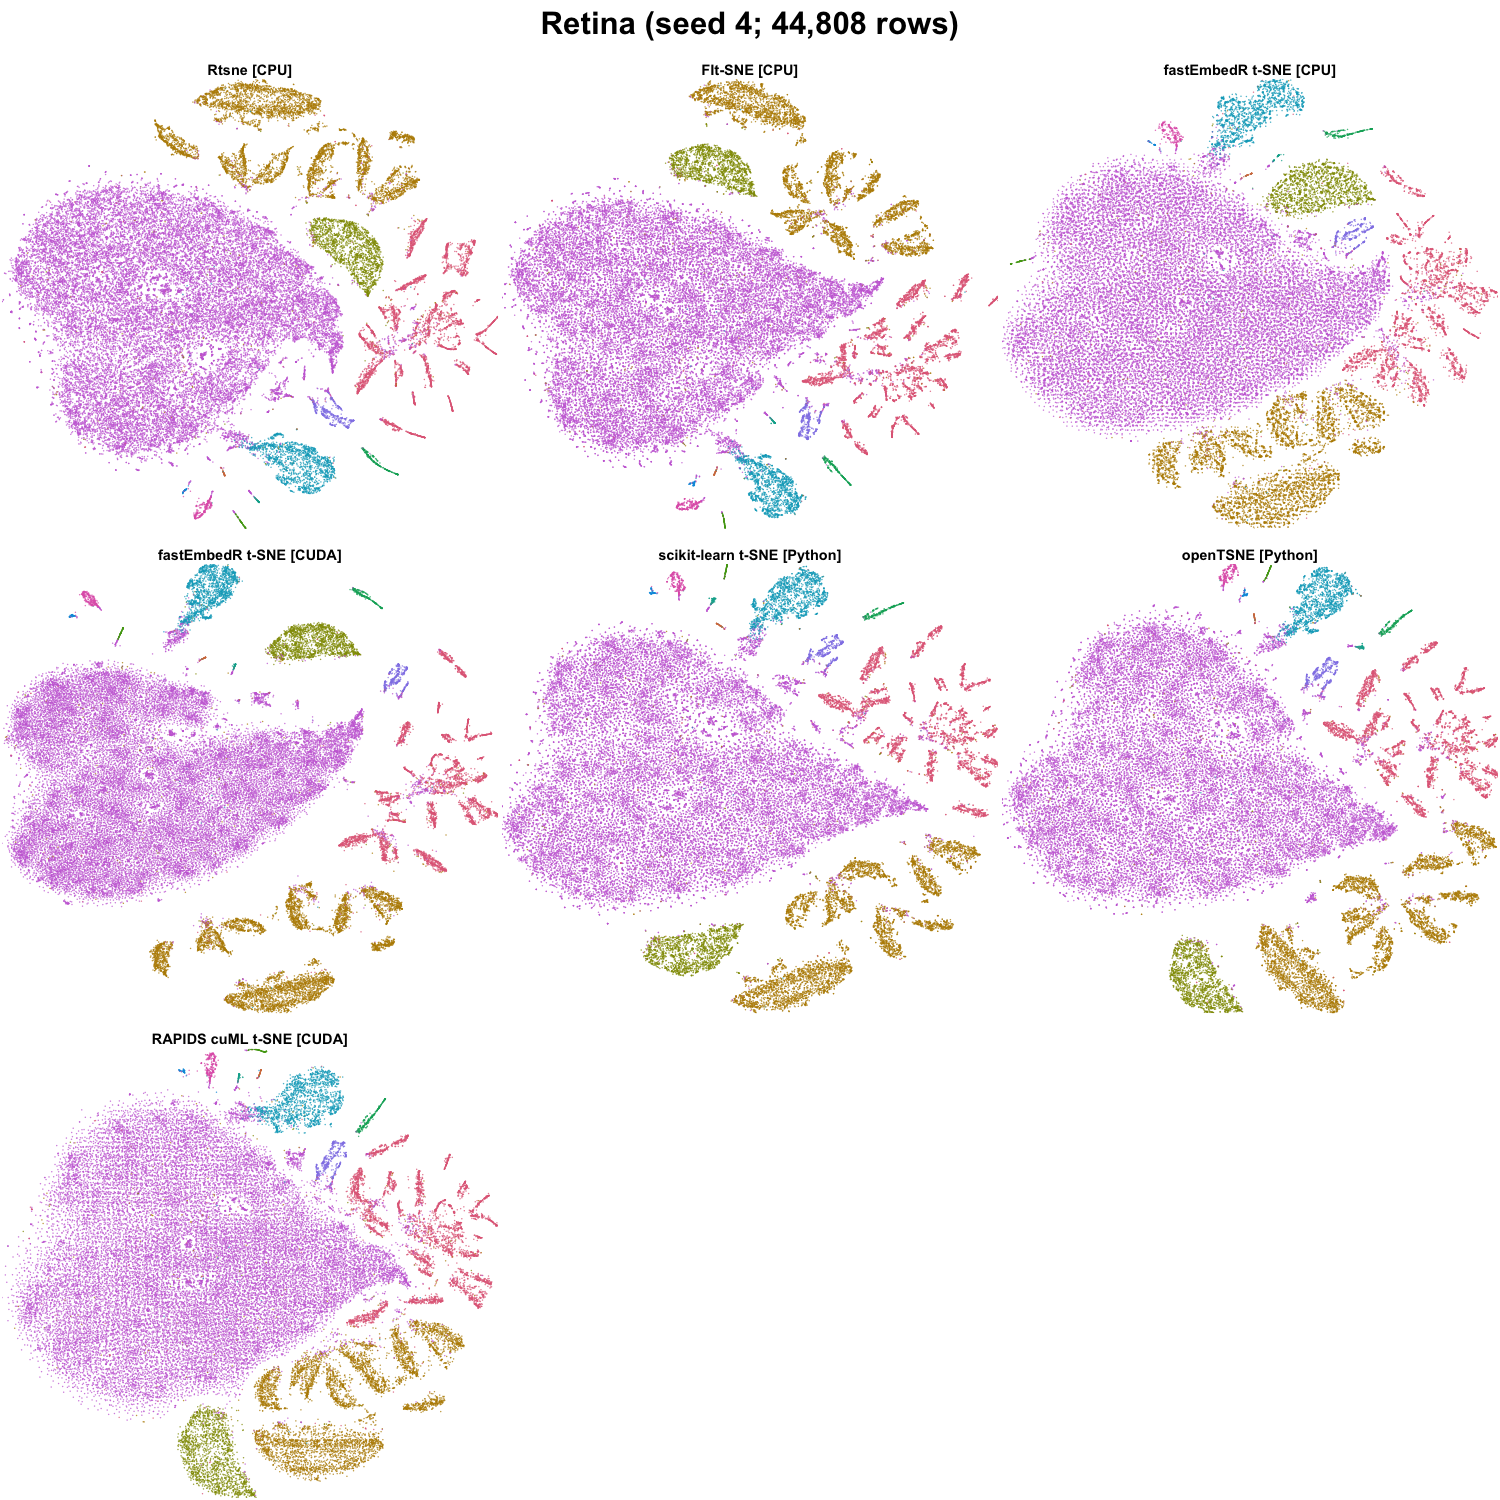
\includegraphics[width=0.94\textwidth]{figures/embedding_all_methods/Macosko2015_retina_tsne.png}
\caption{Retina t-SNE outputs for the tested methods (seed 4; 44,808 rows). Colors encode benchmark labels and were not used for fitting.}
\end{figure}
\clearpage

\begin{figure}[p]
\centering
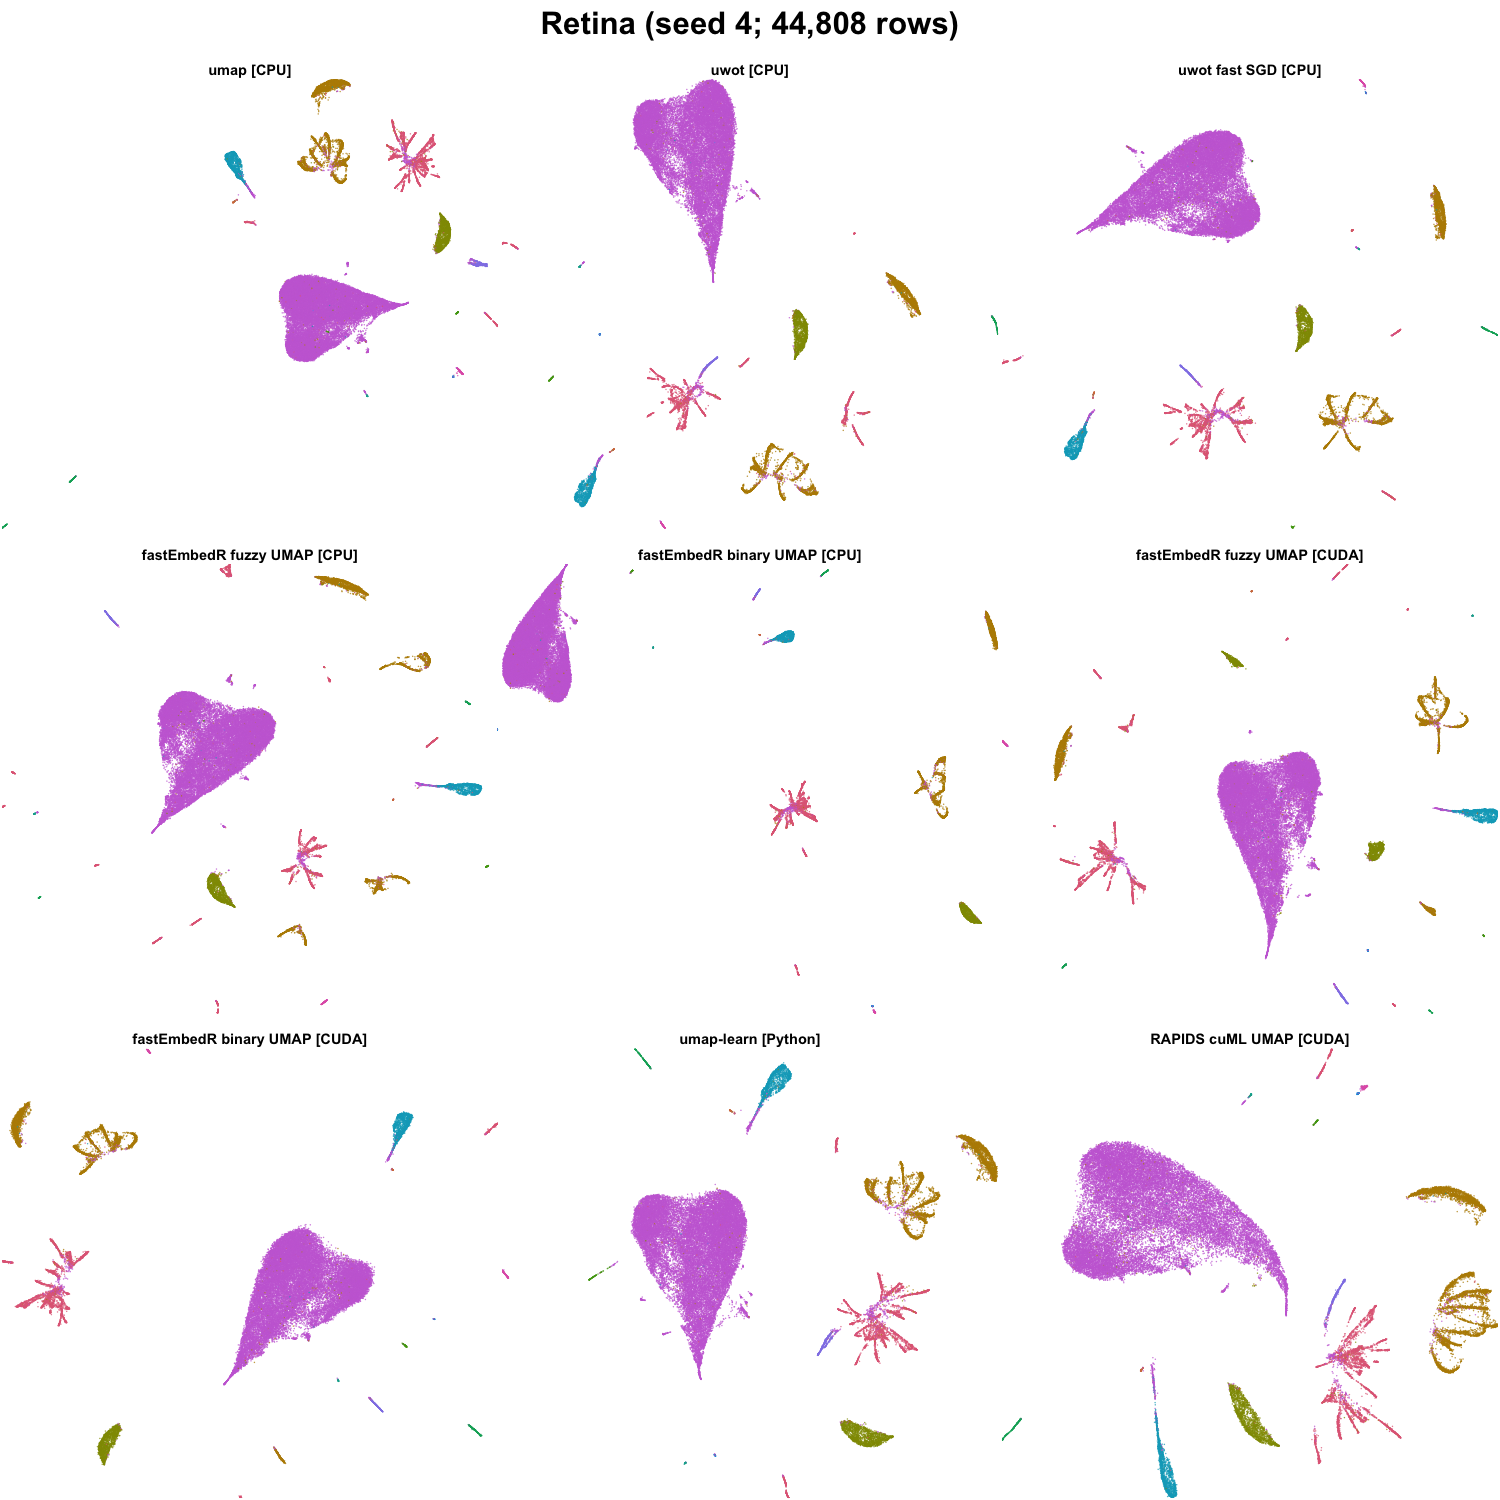
\includegraphics[width=0.94\textwidth]{figures/embedding_all_methods/Macosko2015_retina_umap.png}
\caption{Retina UMAP outputs for the tested methods (seed 4; 44,808 rows). Colors encode benchmark labels and were not used for fitting.}
\end{figure}
\clearpage


\end{document}
